\documentclass{report} % Add the document class
\usepackage{graphicx} % For including graphics like logos
\usepackage{subcaption}
\usepackage{lipsum}   % For dummy text
\usepackage{setspace} % For line spacing
\usepackage{fancyhdr} % For custom headers and footers
\usepackage{geometry} % For page margins
\usepackage{amsmath} % For mathematical equations
\usepackage{enumitem} % For customized lists
\usepackage{amsfonts} % For the \forall symbol
\usepackage{multicol} % For multiple columns if needed
\usepackage{enumitem} % For customizing lists
\usepackage{hyperref} % For hyperlinks for table of contents
\usepackage{acronym} % For defining acronyms
\usepackage{tocbibind} % For adding list of figures, tables to table of contents
\usepackage{tabularx} % For tables
\usepackage{float} % For tables
\usepackage{longtable}%to split tables over multiple pages
\usepackage{array}
\usepackage{booktabs}
\usepackage{caption}
\usepackage{hyperref}
\usepackage{fancyheadings}
\usepackage{multirow}
%
\pagestyle{fancy}
\fancyhead[R]{
    
\includegraphics[width=0.1\textwidth]{./ReportImages/thws_logo.png} % Adjust path and filename
}
\fancyhead[C]{} 
\fancyhead[L]{} 
\addtolength{\headwidth}{\marginparsep}
\addtolength{\headwidth}{\marginparwidth}

\geometry{top=1in, bottom=1in, left=1in, right=1in} % Set page margins

% Configure the hyperref package to remove red boxes and customize link colors
\hypersetup{
    colorlinks=true,      % Set to true to enable colored links
    linkcolor=black,       % Color for internal links (sections, pages, etc.)
    citecolor=black,       % Color for citation links
    filecolor=black,       % Color for file links
    urlcolor=black         % Color for URL links
}


\begin{document}

% Title Page
\begin{titlepage}
    \centering
    \vspace*{1cm}
    
    \Large \textbf{Technical University of Applied Sciences Würzburg-Schweinfurt (THWS)}\\
    \vspace{0.5cm}
    \Large Faculty of Computer Science and Business Information Systems\\
    \vspace{1cm}
    
    \huge \textbf{Master Thesis}\\
    \vspace{1.5cm}
    
    \Huge \textbf{Electrical Engine Efficiency Prediction Bypassing Finite Element Analysis}\\
    \vspace{2cm}
    
    \large \textbf{Submitted to the Technical University of Applied Sciences Würzburg-Schweinfurt in the Faculty of Computer Science and Business Information Systems to
    complete a course of studies in Master of Artificial Intelligence}
    
    \vspace{1cm}
    
    \huge Lilly Abraham\\
    \huge K64889\\
    \vspace{1cm}
    \large Submitted on: 11.12.2024\\
    
    \vfill
    
    \large
    Initial examiner: Prof. Dr. Magda Gregorová\\
    Secondary examiner: Prof. Gracia Herranz Mercedes\\

\end{titlepage}

\newpage % Start a new page


% Including an image on this page
\begin{figure}[h]
    
\includegraphics[width=0.8\textwidth]{./ReportImages/qrcode.png} % Adjust path and filename
    \label{fig:your-image}
\end{figure}

\newpage % Start a new page

\chapter*{Abstract}
\addcontentsline{toc}{chapter}{Abstract}

The thesis explores an approach to predict Key Performance Indicators (KPI)s of topology invariant Interior Permanent Magnet Synchronous Motors 
(PMSM) Electric Motors from its geometric, physical and simulation parameters.
We intend to model the dynamics of Electric Motor functionality by creating surrogate models trained with Finite Element Method (FEM) simulations from its parametric description.
The KPIs to be predicted are vectors of numerical values which can be displayed as the Torque curve(2D) and the Efficiency grid(3D) respectively.
We note the relationship between the Torque curve and the Efficiency grid and incorporate our learnings of both the KPI's nature into our solutions's modelling. \\
We aim to first parameterize the Electric Motor design such that it is feasible to convert into a tabular representation. \\
Next, we would create a table with relevant attributes and design a Multi Linear Perceptron(MLP) to train it in a supervised manner.\\
Subsequently we will regularize the loss functions in a way that would smoothen out the plot curves for both the KPIs. \\
Then we will evaluate the predictions with the test target values by experimenting with various hyperparameter tuning settings 
and as a baseline with the average of the parameters.\\
Additionally we conduct a study to model the task as its graph representation and use Graph Neural Networks(GNN) to predict the KPIs.\\
Lastly we will enable the KPI's plot visualization in a manner presentable to the client Valeo(Automaker Company specializes in manufacturing electric motors for cars).\\

\newpage 

\newpage 

\chapter*{Acknowledgement}
\addcontentsline{toc}{chapter}{Acknowledgement}
I would like to thank my supervisor Prof. Dr. Magda Gregorová for her guidance and support throughout the course of this thesis.
Her dedication and commitment to our work has been inspiring to me especially on how we transformed statistical math into modelling that I might have developed a 
new love for academia. I would also like to express my sincere gratitude to Valeo for providing us with the dataset.
Special thanks are in order to Daniel and Leo for sharing valuable insights of the data from an electromechanical standpoint and for giving me a detailed understanding 
of my task. My Family have been very instrumental in making it possible for me to pursue a Master's degree outside my home country and their endless support throughout 
enabled me to get to my thesis moving in the right direction. Finally, I humble myself before God Almighty for all his blessings and for giving me the strength 
to persevere and bring my dreams to fruition.

\newpage

\newpage

\begin{spacing}{1.2}
    \tableofcontents
\end{spacing}

\newpage

\newpage

\chapter*{Abbreviations}
\addcontentsline{toc}{chapter}{Abbreviations}
\begin{acronym}[TDMA]
  
    \acro{GNN}{Graph Neural Network}
    \acro{MLP}{Multi Linear Perceptron}
    \acro{KPI}{Key Performance Indicator}
    \acro{EM}{Electric Motor}
    \acro{FEA}{Finite Element Analysis}
    \acro{CNN}{Convolution Neural Network}
    \acro{D}{Dimension}
    \acro{MSE}{Mean Squared Error}
    \acro{RMSE}{Root Mean Squared Error}
    \acro{NaN}{Not a Number}
    \acro{ReLU}{Rectified Linear Unit}
    \acro{GPU}{Graphics Processing Unit}
    \acro{MP}{Message Passing}
    \acro{PDE}{Partial Differential Equation}
    \acro{PMSM}{Permanent Magnet Synchronous Motor}

\end{acronym}

\newpage

\newpage

\chapter{Introduction} 
In the design of \acl{EM} (\ac{EM})s, vast amounts of data are generated to determine which design of an \ac{EM} fits best to \acl{KPI} (\ac{KPI})s.
\ac{PMSM}s are largely classified as Surface Mounted \ac{PMSM} and Interior \ac{PMSM}.

\ac{KPI}s of an \ac{EM} are its representative characteristics of a motor drive and is essential to judge the performance of the motor before manufacturing.
Traditionally these \ac{KPI}s are inferred from the description of an \ac{EM} design using \ac{FEA} simulations by approximating the solutions of the Maxwell's equations which are essentially \ac{PDE}. \\
The Torque multiplied by the speed gives an insight of the total power of the motor
The Efficiency map is a behavior map that expresses the motor efficiency function in the torque-speed domain of an \ac{EM}.
One would calculate such kind of behavior maps when there are multiple operating points to consider the motor's drive cycle.
The other \ac{KPI}s such as Losses and Torque ripple are also behavior maps similar to the Efficiency \ac{KPI}.
The paper in \cite{ETA-2021} also cites that the efficiency vs torque and speed map is most representative of the characteristics of the \ac{EM}. 

\ac{FEA} simulations are numerical methods that discretize the geometric parameters of an \ac{EM} into finite elements and solve the \ac{PDE}s for each of them.
This is typically done to simulate the magnetic field distribution of the \ac{EM} and thus assists to generate its \ac{KPI}s.  
It requires domain knowledge in motor physics and complicated setup to run simulations typically in Matlab.

In computational electromagnetics, deep learning can be seen as the most eligible surrogate of \ac{FEA} simulator as they can
provide almost accurate results in relatively no time. 
This is because the \ac{FEA} simulations may take hours to days as it needs to generate for all operating points in the Efficiency map.
Despite the computational burden it comes with, the authors from \cite{FEA-ETA-2017} defends that \ac{FEA} is most appropriate to 
generate \ac{EM} efficiency maps in terms of accuracy based on experimenting overall error rates across operating ranges for different \ac{EM} losses.
FE-based ANN models have been utilized for predicting stress distribution in a 3D printing process [30], bend angles in laser-guided bending [31], 
and performance of a thermoelectric generator [32], for example.\cite{SM EMT-2020}

This process, though well established in the \ac{EM} design is very resource intensive, time consuming and does not allow for high-throughput engine design optimization. 

The actual engine data of Valeo is used here as the dataset comprising of multiple variant designs of the Double-V topology.
Figure \ref{fig:Valeo Motor Structure} depicts the structure of a \ac{EM} manufactured by Valeo. 
The rotor rotates around the Stator to produce the magnetic field whereas the Stator is the stationary part that generates the force to rotate the Rotor.         
\begin{figure}[H]
    \centering
    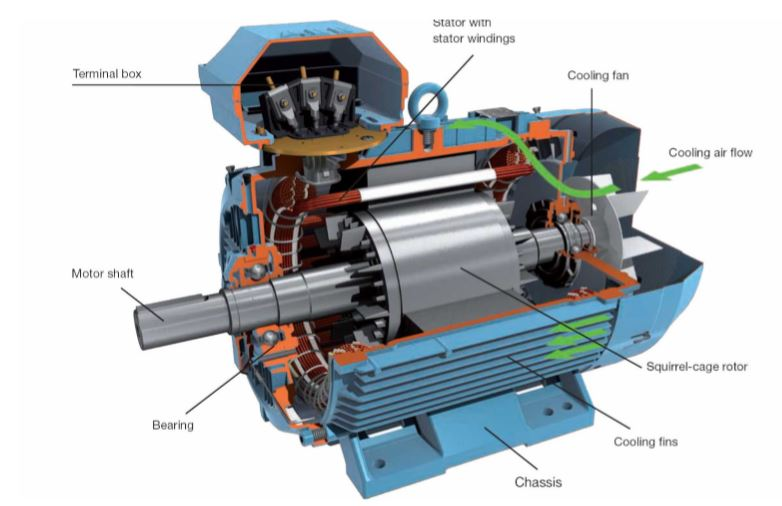
\includegraphics[width=0.75\textwidth]{./ReportImages/ValeoMotorStructure.jpg} 
    \caption{\ac{EM} Motor (Source : Valeo)}
    \label{fig:Valeo Motor Structure}
\end{figure}

The 3 motor topologies manufactured by Valeo are displayed in Figure \ref{fig:EM Magnet Topologies}:
\begin{enumerate}
    \item Single V Magnet - Consists of a single V magnet shown in Figure \ref{fig:V1 Magnet}.
    \item Double V Magnet - Consists of double V magnets shown in Figure \ref{fig:V2 Magnet}.
    \item Nabla Magnet - Consists of a single V Magnet and a delta magnet shown in Figure \ref{fig:Nabla Magnet}.
\end{enumerate}

\begin{figure}[H]
    \centering
    \begin{subfigure}{0.32\textwidth}
        \centering
        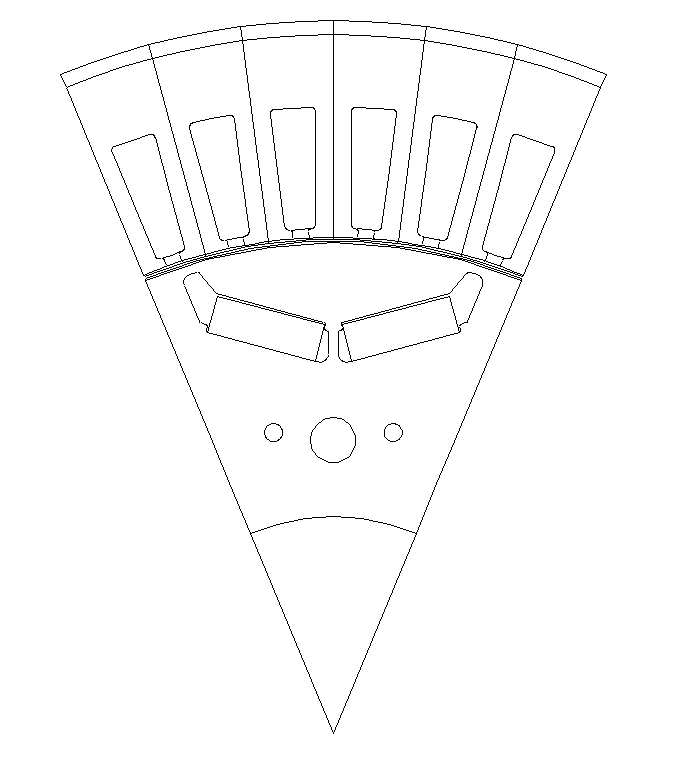
\includegraphics[width=\textwidth]{./ReportImages/1V_Magnet.png}
        \caption{Single V Magnet}
        \label{fig:V1 Magnet}
    \end{subfigure}\hfill
    \begin{subfigure}{0.32\textwidth}
        \centering
        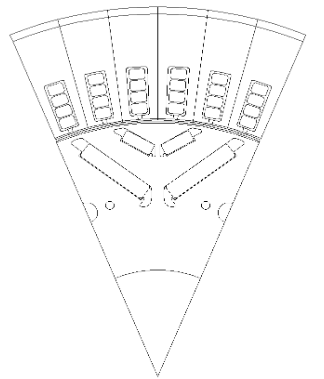
\includegraphics[width=\textwidth]{./ReportImages/2V_Magnet.png}
        \caption{Double V Magnet}
        \label{fig:V2 Magnet}
    \end{subfigure}\hfill
    \begin{subfigure}{0.32\textwidth}
        \centering
        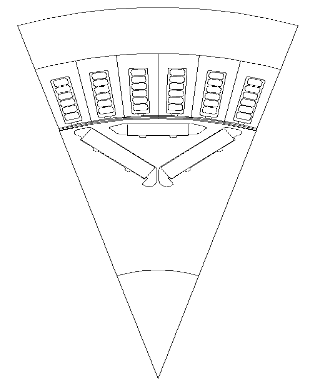
\includegraphics[width=\textwidth]{./ReportImages/Nabla_Magnet.png}
        \caption{Nabla Magnet}
        \label{fig:Nabla Magnet}
    \end{subfigure}
    \caption{\ac{EM} Magnet Topologies (Source : Valeo)}
    \label{fig:EM Magnet Topologies}
\end{figure}

Figure \ref{fig:Torque Curve} and Figure \ref{fig:Efficiency Grid} give a glimpse of the \ac{EM} \ac{KPI}s to be predicted.
\begin{figure}[H]
    \centering
    \begin{minipage}[b]{0.44\textwidth}
        \centering
        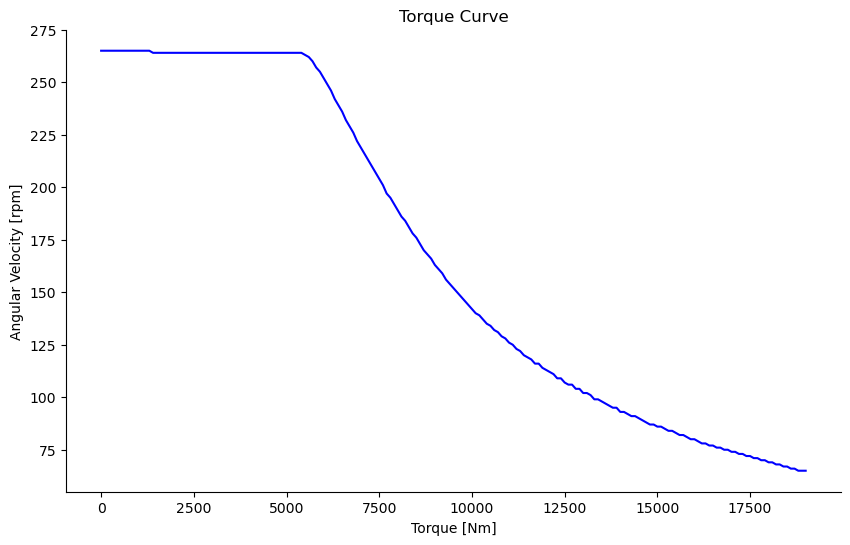
\includegraphics[width=\textwidth]{./ReportImages/TorqueCurve.png}
        \caption{Torque Curve} % Center the caption here
        \label{fig:Torque Curve}
    \end{minipage}
    \hfill
    \begin{minipage}[b]{0.54\textwidth}
        \centering
        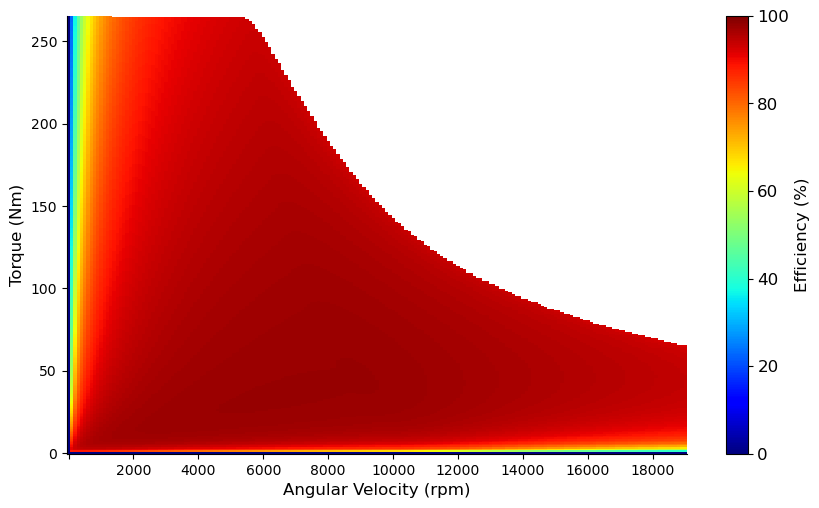
\includegraphics[width=\textwidth]{./ReportImages/EfficiencyGrid.png}
        \caption{Efficiency Grid}
        \label{fig:Efficiency Grid}
    \end{minipage}
\end{figure}

We can observe the relation between the Torque curve and the Efficiency grid. 
The values within the Efficiency envelope can be understood with the different contour shades whose level of shading is shown to the right.
Most importantly we can also make out that the Efficiency envelope is of the same shape as the Torque curve.

Figure \ref{fig:EM Design Flowchart} gives an outlook of both the current approach and our proposed approach to generate the \ac{KPI}s.
We discuss each component of the flowchart below :
\begin{enumerate}
    \item \textbf{\ac{EM} designs parameterized} \\
    The design of each of the \ac{EM} variants described parametrically for its geometric, physical and simulation features are considered as the input.
    \item \textbf{Current Approach}
    Approach followed currently by Valeo.
    \begin{enumerate}
        \item \textbf{Matlab Script 1} \\
        Creates a design mesh from the parametric description of the \ac{EM}'s geometric and physical features.
        \item \textbf{\ac{FEA} simulator} \\
        Multiple \ac{FEA} simulations which are by nature \ac{PDE} is done on this mesh. The \ac{FEA} solver then 
        generates the byproducts associated with the magnetic flux of the \ac{EM}.
        \item \textbf{Matlab Script 2} \\
        The outputs from the \ac{FEA} simulations are then post processed and the intermediary outputs which are matrices of values in mat format are fed to the next stage.
        \item \textbf{Motor Builder} \\
        Another round of post processing is done on the magnetic flux products to generate the Power and Torque associated with the \ac{EM} design.
        Motor builder settings such as length of the motor, maximum rotation speed as well as electrical settings for e.g. input voltage and current are given to 
        generate the \ac{KPI}s. The Motor Builder also is a GUI that provides visualization of the \ac{KPI} plots to the designer.
    \end{enumerate}
    \item \textbf{Proposed Approach}
    Approach we undertake as surrogate modelling.
    \begin{enumerate}
        \item \textbf{Data Preprocessing} \\
        The input features typically as its numerical equivalent is preprocessed and converted into its tabular representation such that it is suitable to be fed into the Neural Network.
        For training the network, additionally the targets are taken from the \textbf{Matlab Script 2} which also serves as the ground truth represented as a dotted line.
        \item \textbf{Neural Network} \\
        We use \ac{MLP} as our deep learning model which is made up of fully feedforward connected layers. For training, also the targets are considered to minimize the loss of the predictions to be generated.
        However for inference, only the inputs are used to generate its approximated targets.
        \item \textbf{Data Postprocessing} \\
        The predictions generated by the neural network is post processed to be similar to the targets of the \textbf{Matlab Script 2} in terms of dimensions and is plotted.
    \end{enumerate}    
    \item \textbf{KPI Plots} \\
    The targets which are vectors of numerical values are displayed graphically.
\end{enumerate}

This master thesis explores a way to do light weight surrogate modelling of the current process as is highlighted in Figure \ref{fig:EM Design Flowchart} by 
exploiting data-driven deep neural networks to approximate the \ac{KPI}s derived from \ac{FEA} simulations.

\begin{figure}[H]
    \centering
    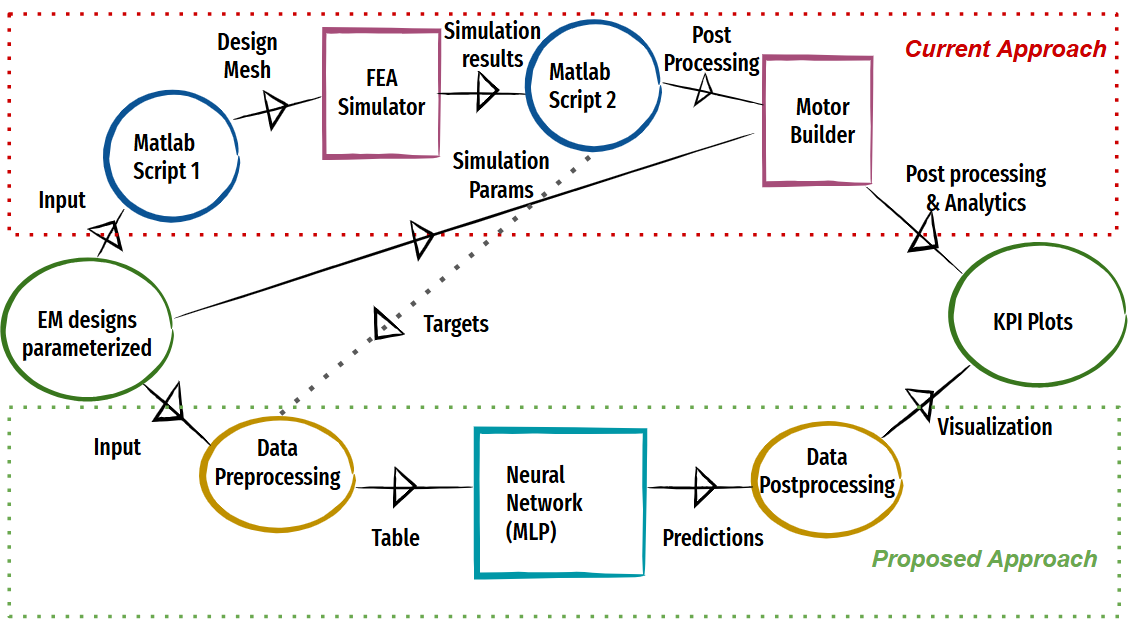
\includegraphics[width=1\textwidth]{./ReportImages/EM_design_flowchart_v2.png} 
    \caption{EM Design Flowchart}
    \label{fig:EM Design Flowchart}
\end{figure}

Complete replacement of \ac{FEA} simulations with deep learning models is not feasible however we can exploit the use of deep neural networks 
trained on \ac{FEA} simulated data to reduce the computation burden of running these simulations repeatedly in the future.
The inverse step of generating the motor designs is most useful for companies as they can get a feel of what the best designs would look before manufacturing them.

\section{Objective}\label{sec:Objective}
The objective of our work is to verify whether surrogate modelling to replace \ac{FEA} simulations is feasible.
Our task is a supervised learning task to predict 2 KPIs namely the Torque curve and the Efficiency grid which are vectors of numerical values  
from the parametric description of topology invariant \ac{EM} and \ac{FEA} simulated KPIs as ground truth. 
The remaining \ac{KPI} such as Costs, Vibration losses, Torque ripple etc., can be calculated from these 2 KPIs for instances the losses are inversely proportional to the Efficiency values.
The Torque curve is a vector of torque values across angular velocity ranges which can be visualized as a a 2D plot whereas the Efficiency grid is a matrix of 
dimensions (torque ranges $\times$ angular velocities ranges) and can be visualized as 3D heatmap of contour plots. 
Both the \ac{KPI}s are continuous values which makes our task a regression problem. 

\section{Motivation}\label{sec:Motivation}
Our motivation to undertake this thesis is to lay the ground work for generating \ac{EM} designs in the future. To our knowledge, there has been no work yet on Generative 
AI in the domain of \ac{EM} designs. The research goal would be to condition the generative model on the predicted \ac{KPI}s to be able to self generate the most efficient \ac{EM} 
designs. From an application standpoint, it would be beneficial for Automaker companies to refer the generated \ac{EM} designs to be able to suggest the most appropriate \ac{EM}s 
for automobiles as per customer requirements for instance the horsepower of the car.

\section{Problem Statement}\label{sec:Problem Statement}

Given our Data $\mathcal{X}  = [x_1, x_2, ..., x_{n}]^T \in \mathbb{R}^{n}$, where $n$=89 is the number of parameters of the \ac{EM} designs, we attempt to approximate the targets, 
Torque curve as $\mathcal{Y}_1 = [y_1, y_2, ..., y_{h}]^T \in \mathbb{R}^{h}$ where $h$ denotes the number of participating angular velocities and 
Efficiency map as $\mathcal{Y}_2 \in \mathbb{R}^{w \times h}$ representing a grid of efficiency values defining the operating range of the \ac{EM}, where $w$ refers to 
different torque levels and $h$ the angular velocities. Each element $\mathcal{Y}_2(i,j)$ represents the efficiency at torque level $i$ and angular velocity $j$. 

We list down the challenges we had faced when modelling our problem as follows : 
\begin{enumerate}
    \item Since we have 2 targets of continuous values to predict ours is now a multi regression problem. The model architectures in Section \ref{sec:MLP Model} 
    shines light on how we go about it.
    \item The Torque Curve typically harbours integers values albeit our task is in essence a regression problem which primarily works with floating point values. 
    Section \ref{sec:MLP Model} discuss how we tackle this challenge. 
    \item The dimensions of the Efficiency grid differ across \ac{EM} variants. However the targets which has to be supplied to the model needs to be of a fixed size.
     We discuss in Section \ref{subsec:Deep Dive into 3D KPI} how we mitigate this problem.
    \item The ranges among the 1st and 2nd target vary significantly and is yet another challenge we overcome in Section \ref{sec:Loss for 3D KPI}.
\end{enumerate}

\section{Research Question}\label{sec:Research Question}

We were skeptical on building a model architecture wherein the 2nd KPI is dependent on the 1st KPI as typically the former's shape is dependent on the latter 
and not its values. However we can assume the values within the shape to be non zero values and otherwise 0s and model it in future.

Alternatively we could also build 2 models one for each KPI and thus feed in the dependent predictions when training the latter. 
However, it would be computationally expensive and does not help in the scenario when we might need to generate \ac{EM} parametric descriptions.
Additionally we deemed it unnecessary as the dimensions of the Efficiency grid vary with the torque curve and not necessarily the Efficiency values. 

\section{Thesis Structure}\label{sec:Thesis Structure}

Over the course of the thesis we shall refer the Torque curve as Torque KPI and the Efficiency grid as Efficiency KPI respectively.
The remainder of the thesis is organized to follow sections namely Literature Review, Dataset, Modelling, Experiments and Results, Graph Modelling, Conclusion, 
Bibliography and Appendix.
In Literature Review section will introduce the works that has already been carried out in this domain. 
In the Dataset section a detailed insight is elaborated on how our data is structured .
In the Modelling section, we introduce the network architectures and loss regularization techniques used to tackle the problem.
The outcomes of our work are presented in Experiments and Results chapter in addition to other findings we unearth.
Graph Modelling section is an empirical study which outlines the background of \ac{GNN}s primarily Heterogeneous \ac{GNN}s and defines its concepts. We also attempt to 
present a workflow on how to use \ac{GNN}s for out task.
Conclusion chapter summarizes the thesis briefly and would also give a glimpse into possible areas of improvement. 
Bibliography section lists out the articles cited for this thesis. 
Lastly we share all supplementary information in the Appendix section.

\newpage 

\chapter{Literature Review} 
There has been extensive research in modeling the Electric Motor with \ac{CNN} based on the images of the motor cross-section. \\
However our approach is progressive in the sense that once the \ac{KPI}s are predicted we would like to be able to generate the inputs.\\
Reproducing images is not known to be the best approach given the infamous known fact that AI generated images are faulty. 
However by generating the parameters of the motor we can be rest assured of more precise results. 
Hence the need to focus on the inputs as they are with their parametric description.
Vivek et al. in \cite{VAE-MT-2021} also highlights that predicting \ac{KPI}s with tabular data is significantly more efficient than using the images because the latter could result 
in less accurate designs due to the need of high resolution images in addition to its overall computation cost required for training. Their work 
involves the use of a Variational Autoencoder to predict the \ac{KPI}s with an \ac{MLP} as well as sample the latent space to generate new \ac{EM} designs.\\
Evolutionary algorithms such as genetic algorithms are traditionally used as multi objective optimization algorithms to generate the designs by iteratively
updating the design parameters whereas the \ac{FEA} simulations evaluate the performance of each design. 
The optimization algorithms are itself incredibly time consuming because fitness evaluation will need to be performed multiple times with \ac{FEA}.
In addition a larger number of iterations of these algorithms is necessary to evaluate each design candidate in order to explore the entire design space.
We do surrogate modelling of the \ac{FEA} simulations which serves as the baseline to eliminate the role of evolutionary algorithms as well for generating designs.
The latter could potentially be a future work to be carried out since the time complexity associated with the Genetic Algorithms 
may discourage users to wait until convergence and rather persuade them to be satisfied with a suboptimal design.\\
Marius et al. in \cite{VAE-MT-2021} undertake works on optimizing electric motor design generation by compressing its parametric description 
across multiple topologies into a compressed latent space thereafter from which new \ac{EM} designs can be sampled.
They also disclose the solutions taken to address the problem wherein unique parameters of 1 topology are absent in another topology.
They mitigate this concern with 2 approaches. Firstly, they default the missing values with an arbitrary fixed constant 0s this inturn 
pushes the model to learn a nonsensical value for irrelevant features.
However they also note that this shortcut results in wasting model capacity making the learning unnecessarily more difficult.
Therefore, they have also used a second approach termed as Masked Learning Process wherein only features relevant for the motor topology are 
considered for modelling loss reconstruction of the model. \\
The authors of \cite{EM 2DFMP-2022} presents a method to predict 2\ac{D} flux maps of an Interior \ac{PMSM} using classical machine learning ensemble regression models.
Therefore for each coefficients of the 2\ac{D} flux maps, a separate regression model is trained which are then ensembled to make target predictions. 
Although there are classical Machine Learning models which handle multi regression, they do not perform very well with higher dimensions as 
opposed to deep neural networks. The writer also points out that these models fare better than deep neural networks when it comes to data required and training time.\\
Similar to our usecase for modelling \ac{EM} for cars,the writers of \cite{ETA-V-2020} experiments to compute the efficiency map of Toyota Prius have 
been computed. The methodology used is to observe Magnetic field flux density to predict how it evolves over time for different operating points of the map.
The paper \cite{HMLO-2021} also examines a study of how a machine learning observer can augment the performance of torque estimation of 
induction motors trained with deep neural networks.
The motivation behind using the observer is made by domain aware knowledge that the torque estimated depends on the stator's magnetic flux.
The authors claim to have made this possible by incorporating the information of speed, voltage and current into the network to realize the \ac{EM}'s torque.
They also indicate that physics modelling of the network enabled them to develop light-weight models with better accuracy.\\
In \cite{EM SM-2023}, the authors compare and evaluate the performance of surrogate modelling Surface Permanent Magnet's parametric and image based designs.
Their experiments conclude that \ac{MLP}s trained on the parametric description can better infer targets such as Induced Voltage and harmonic distortion 
that are linearly dependent to the designs when compared to cogging torque which is not.
To learn the non linear functions, they also experimented with \ac{CNN}s which could infer all targets just as well as it inherently takes 
into account the pixel spatiality from motor designs as RGB images. In addition they built a hybrid model to utilize the image and parametric 
description but have comparable reported performance with that of \ac{CNN}s.
They also suggest a slight decline in accuracy for a linearly dependent target for the \ac{CNN} model as image resolution constrained the precision of the inputs.\\
Existing literature also covers works on modelling this work as tabular data using \ac{MLP}s. \\
We review the concept of surrogate modelling and its applications in \ac{EM} domain.
The researchers of \cite{SM EMT-2020} talks about the use of domain knowledge to improve the accuracy of surrogate modelling \ac{EM} by creating a hybrid of both 
physics and data driven based models.
In addition, it presents a workflow for surrogate modelling the air gap torque from \ac{FEA} simulated data and compares and contrasts the computationally efficiency with regards to both approaches. 
Similarly, Yusuke et al. in \cite{PANN-MT-2021} and \cite{PANN-MOO-2021} also claim that a physics assisted neural network significantly improved the accuracy performance when predicting the cogging torque 
of Permanent Magnet Synchronous Motors. Their experiments suggest that approximating the cogging torque with a linear subdomain model which serves as an additional 
input to the neural network when making the final prediction. With this methodology, they also disclose that a significant less data than estimated suffice.
Works by \cite{EM TL-2020} explores methodologies to extend an already model to predict efficiency maps for a topology it was untrained for by exploiting 
the concept of transfer learning. The writers claim to get this accomplished by mixture of greedy pretraining and then overall finetuning the model.
They do so by freezing the pretrained network which they identify as common knowledge so that gradient flow is disabled and substitute the other 
layers of the pretrained model with new layers which is essential for the new task.
In addition to a topology change, this paper also explore transfer learning for different label than the pretrained model given that the labels are similar in nature to each other. 
This eventually assist the model to generalize better and conserve the time it would have spend training from scratch by knowledge reusing. 
Finetuning is a also a boon when the dataset for the new topologies are limited in existence.\\
Furthermore, research by \cite{EM CNN-2024} also presents their approach on handling surrogate modelling of topology invariant Interior 
Permanent Magnets motors to predict its Torque characteristics.
Generally the topology differs based on the count of the magnets, this is evident from the Figures in \ref{fig:EM Magnet Topologies}.
The writers claim to have used the cross-sectional images of motor designs in addition to the magnetic flux distribution of the Stator as input to the
inputs to train the \ac{CNN}. The auxiliary input is supplemented by \ac{FEA} simulations which is enriched with the nature and placement of 
the magnets in the Rotor. Although, the \ac{FEA} is used yet the product here is generated quicker and thus does not add on largely to its overhead on time complexity. 
They also claim to have improved the generalization performance of \ac{CNN}s with this strategy. In addition they suggest such domain knowledge modelling decisions 
can also be beneficial for both parameter and topology optimization of \ac{EM} as well as for prediction of its other \ac{KPI}s.\\
Arbaaz et al. in \cite{DL-ETA-2019} also tries to generate the efficiency map by first generating its flux linkage maps and the torque curve 
thus accounting for geometric and operating point variations. Two interesting points are made in this paper.
First, as the number of excitation points vary across designs, thus a model suitable for handling variable input sequence length is needed.
Meaning the values only within the torque curve i.e., excitation points are predicted. This results in conserving training time when predicting a fixed sized grid
They also use confusion matrix for efficiency threshold so designer can filter out efficiencies in the operating range one is most eager to find out.
Secondly, for efficiencies being predicted outside the excitation points, the authors propose to provide an uncertainty measure to quantify confidence level using Monte Carlo dropout.
Reason being the error rate in the efficiency grid is maximum at the envelope of the curve. This factor gives the end user 
the flexibility to choose to generate the \ac{KPI}s with the \ac{FEA} simulations or the surrogate model.\\
Studies in \cite{EM-PM-2020} presents an interesting take on evaluating the performance of \ac{EM} with electrical engineering inspired benchmarks.
They highlight the inadequacy of evaluations generated by classical Machine Learning approaches such as \ac{MSE}, R2 Score and Symmetric Mean Absolute Percentage Error.
The argument is that these metrics favor the static area in the \ac{KPI}s which are relatively easier to predict.
Meanwhile the dynamic areas in the \ac{KPI}s is not projected as much having less dominance with respect to coverage area.
They experimented this finding with Induction Motors to generate its Torque Vs Speed Predictions. The dynamic parts they considered 
were typically the regions in the curve before saturation is achieved. 
In such cases the Machine Learning metrics could give an over optimistic score when compared to Electrical Engineering designed metrics.\\
Researchers in \cite{DL-MF-2019} also discusses approaches to judge the accuracy with a physics aware metric for estimating 
magnetic field of low frequency electromagnetic devices. The do so by quantifying the uncertainty of the predictions by adding 
a probabilistic component to the wights of the neurons in the network architecture. This technique they employ is called Monte Carlo dropout 
with which they generate uncertainty maps. 
The distribution of the predictions they thus generate more closely approximate that of the same generated by \ac{FEA} simulations as the accuracy improves.
Interestingly they also discuss the possibility of modelling the usecase with Graph Convolutional Networks instead of \ac{CNN}s.
They suggest that rather than images, graphs are better suited as they can handle unstructured design mesh which is 
typically fed into the \ac{FEA} simulator as is shown in the Figure \ref{fig:EM Design Flowchart}.\\
The writers of \cite{ETA-LA-2020} emphasize the importance of having a very low error rate for the Efficiency Maps by \ac{FEA} simulations 
as the drive range of a vehicle's efficiency is determined with this \ac{KPI}. 
The Efficiency \ac{KPI}s generated by the \ac{FEA} simulations are obtained from torque, copper loss iron loss and mechanical loss.
They study methods to further improve the accuracy of \ac{FEA} simulations of Interior Permanent Magnets by modelling the effect 
of losses such as minor hysteresis loss, stray loss, AC loss and manufacturing degradations at different operating points into these simulations.\\
Although this is fairly good foreseeing the impact of generating the inverse process yet \ac{MLP}s cannot necessarily learn all the intricacies within motor components.
Hence the need to better represent the data typically in the form of graphs and model \ac{GNN}s to achieve the desired results. 
Modelling with graphs preserves the spatiality of the design as well as also gives us provision to incorporate the physical and magnetic 
characteristics of the designs if any which would not have been possible with \ac{CNN}s.
There has been close to no work of \ac{GNN}s in this domain. 
However we see progress of \ac{GNN}s in molecular chemistry and social networks usecases from which we draw inspiration.

\newpage 

\chapter{Dataset} 

Valeo has shared 1481 Excel Workbook files for each motor variant of three-phase interior \ac{PMSM} motors with 8 poles and 48 slots. 
Around 89 parameters which comprises of the geometric, physical and simulation properties of the motor are chosen among the 196 parameters depending on its overall variability and significance.
This was a design decision we made based on our understanding of the data.\\
Figure \ref{fig:Full Motor} shows the geometry of a whole Double V motor which can be sliced into 8 identical parts owing to the motor design's rotational symmetry.
\begin{figure}[H]
    \centering
    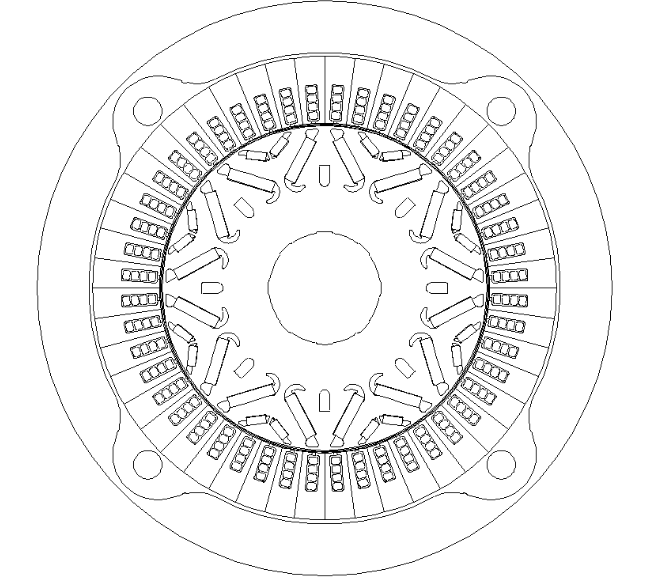
\includegraphics[width=0.5\textwidth]{./ReportImages/FullMotorv2.png} 
    \caption{Complete EM Geometry(Source:Valeo)}
    \label{fig:Full Motor}
\end{figure}
Figure \ref{fig:1/8 Motor Crossection} is a hand drawn sketch showing our understanding of how the geometry of 1/8 cross-section of the same motor looks like.
This comes in handy when creating the graph representation of the motor.
From the Figure, we can make out that the motor very largely is comprised of the Rotor and the Stator separated by the air gap between which the magnetic flux flows.
The Rotor hosts the permanent magnets which when rotated generates the magnetic field. The magnets sits on top of free shaped air pockets in the design. 
The free shape of these air pockets are described geometrically by oblongs which draws the shape geometrically along fixed points.
The Stator comprises of the Stator poles which are 6 in number here. There are 4 slot windings for each stator slot in the tooth shoe, the slots are where the stator windings made 
up of copper sit at. The Stator yoke separates each tooth shoe from the outer radius of the motor.

\begin{figure}[H]
    \centering
    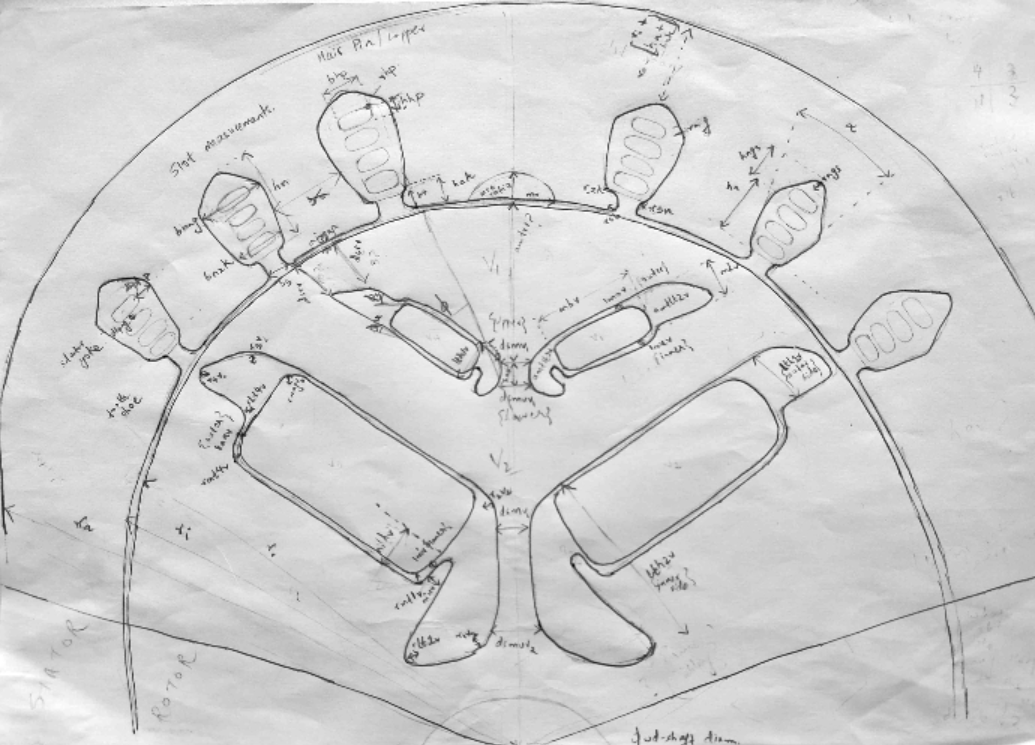
\includegraphics[width=1\textwidth]{./ReportImages/EMCrosssectionFiltered.png} 
    \caption{1/8 Motor Crossection}
    \label{fig:1/8 Motor Crossection}
\end{figure}

\section{Data Preprocessing for \ac{MLP}}\label{sec:Data Preprocessing for MLP}
For modelling the \ac{MLP}, we present the data in tabular form with the parameters corresponding to columns. \\
In order to make the data compatible with our model, some level of data processing was carried out as elaborated below.

\subsection{Data Exploration of the Input Parameters}\label{subsec:Deep Dive into Input Parameters}
All parameters including the additional ones in each topology are considered as a separate columns and therefore if a particular column is topology dependent then the 
column corresponding to the missing data of this topology s treated as 0 values. Defaulting geometrical values as 0 seems to be the most reasonable approach in comparison 
to its standardised norm.
The values are then read and stored as their floating point equivalent to ensure data precision.
Furthermore all degree columns are converted to their equivalent radian values as the latter are directly related to the geometry and makes derivation of other 
parameters much simpler whereas degrees is a notion of denoting a sliced angle.\\ CITE...Explain better

\subsection{Data Exploration of the Torque \ac{KPI}(Torque Curve)}\label{subsec:Deep Dive into 2D KPI}
Figure \ref{fig:Standard Deviation of 2D KPI} shows the standard deviation of few samples of the Torque \ac{KPI} from the entire dataset.
The x-axis represents the angular velocity of the motor ranging from 0 to 19000 rpm. Meanwhile, the y-axis represents the torque values corresponding to the angular velocity.
For our dataset, the range of torque values are between 55 and 280 Nm. We do not start the y-axis from 0Nm as the torque curve stops its decline on reaching torque 
saturation point of 55 Nm and we presumed it best to conserve spacing in the plot.
The mean of all samples of the dataset is displayed with an overlay of how its standard deviation is around the mean.
Furthermore, we display a twin y-axis in red showing the standard deviation of random handpicked samples with the mean.

We make the following observations:
\begin{enumerate}
    \item The \ac{RMSE} is at its peak at low angular velocities.
    This is evident from the Standard deviation ranging up to 3 until 5000 rpm. Beyond which the standard deviation decreases drastically until 
    saturation visible with the plateauing of the curve.
    \item The curve to an extent resembles a mirrored S shape.
    This finding is critical for how we modelled the loss regularization for the target and will be further elaborated in Section \ref{sec:Loss for 2D KPI}
    This finding is critical for how we modelled the loss regularization for the target and will be further elaborated in Section \ref{sec:Loss for 2D KPI}
    \item Samples almost similar to one another
    The samples shown here are almost resembling one another in shape and nature of curve. The finer details are at the points of the curve where it makes its transitions 
    This observation is crucial and directly impacts our  decision on choosing our Baseline model to be discussed in greater detail in Section \ref{sec:Results with Baseline}
\end{enumerate}

\begin{figure}[H]
    \centering
    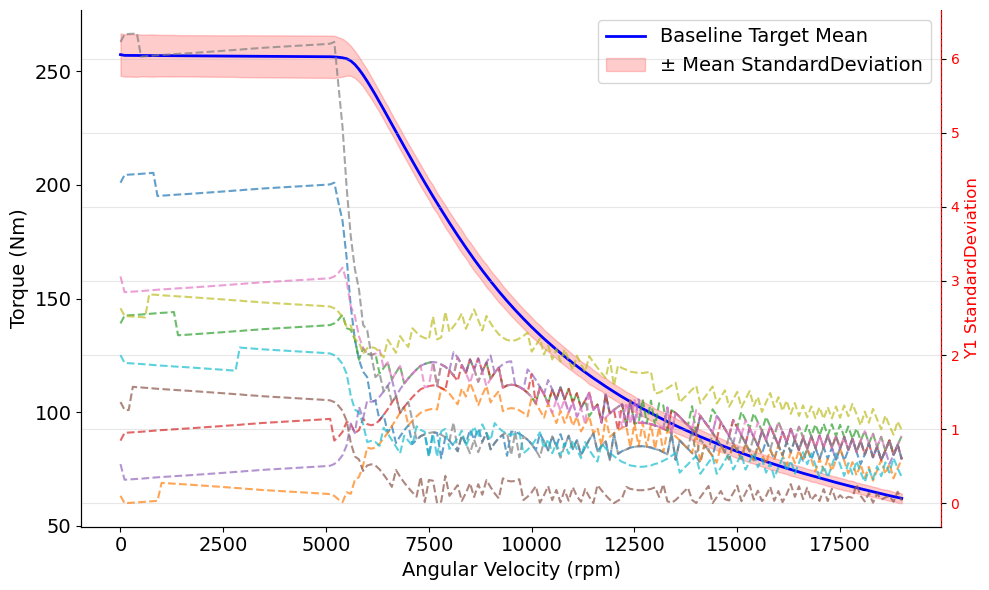
\includegraphics[width=0.75\textwidth]{./ReportImages/StandardDeviation_Baseline_y1.png} 
    \caption{Standard Deviation of 2D KPI} 
    \label{fig:Standard Deviation of 2D KPI}
\end{figure}
\subsection{Data Exploration of the Efficiency \ac{KPI}(Efficiency Grid)}\label{subsec:Deep Dive into 3D KPI}
As the target values of the Efficiency \ac{KPI} are not provided with the correct dimensions we have an additional step which takes the maximum torque value from the Torque \ac{KPI} 
and slices off the Efficiency grid to only range from [-Maximum Torque, Maximum Torque]. 
Subsequently we choose only the rows of the MM grid detailed in Table \ref{tab:Excel File Structure} which correspond to the indices of the sliced efficiency grid.
This step ensures that we grant the model the correct dimensions of the Efficiency \ac{KPI} based on its Torque \ac{KPI}.\\
Figures \ref{fig:Standard Deviation of 3D KPI(Efficiency)} and \ref{fig:Standard Deviation of 3D KPI(Efficiency) Positive Grid} both illustrate the standard deviation 
of the efficiency values plotted against its angular velocity. The standard deviation levels is shown as a scale with colors darkening as the standard deviation increases.
Efficiency values for negative torque values correspond to when motor is in generating mode and those of positive torque values to when motor is in monitoring mode.\\
In both modes, the efficiency is almost similar albeit from Figure \ref{fig:Standard Deviation of 3D KPI(Efficiency)}, we note it is not the case for our dataset. 
This is evident from low angular velocity-high torque distribution area where we can see a clear distinction with \ac{NaN} values.
Since these are \ac{FEA} simulations, it is probably an effect of a post processing step taken by the Motor builder.
This observation made us decide on dropping the negative Efficiency \ac{KPI} and to focus on only predicting the positive Efficiency \ac{KPI}.\\
The latter can be mirrored to replicate the efficiency when it is in generating mode if necessary.
However over the course of this thesis, we donot do so, as it is not relevant to evaluate a duplicate again.
From Figure \ref{fig:Standard Deviation of 3D KPI(Efficiency) Positive Grid}, we can observe the deviation is at its peak at low torques, extreme angular velocities. 
We discuss the modelling of this information in Section \ref{sec:Loss for 3D KPI}. 
We also can observe that beyond the Efficiency envelope, there are no efficiency values and can be translated as blank values in the grid or \ac{NaN} values in the padded Efficiency matrix.
we incorporate this information in Section \ref{sec:Loss for 3D KPI}.
In addition, we notice skewness at the border of the curve within the grid, we discuss in Section \ref{sec:Post Processing} how we handle this scenario.

As we had noted already the Efficiency \ac{KPI} envelope is completely dependent on its equivalent Torque \ac{KPI} curve. 
The area beneath the boundary of which is looked into by the \ac{EM} manufacturers to determine the car's efficiency in the drive range.
This is yet another finding we use in Post Processing as is further elaborated in Section \ref{sec:Post Processing}

\begin{figure}[H]
    \centering
    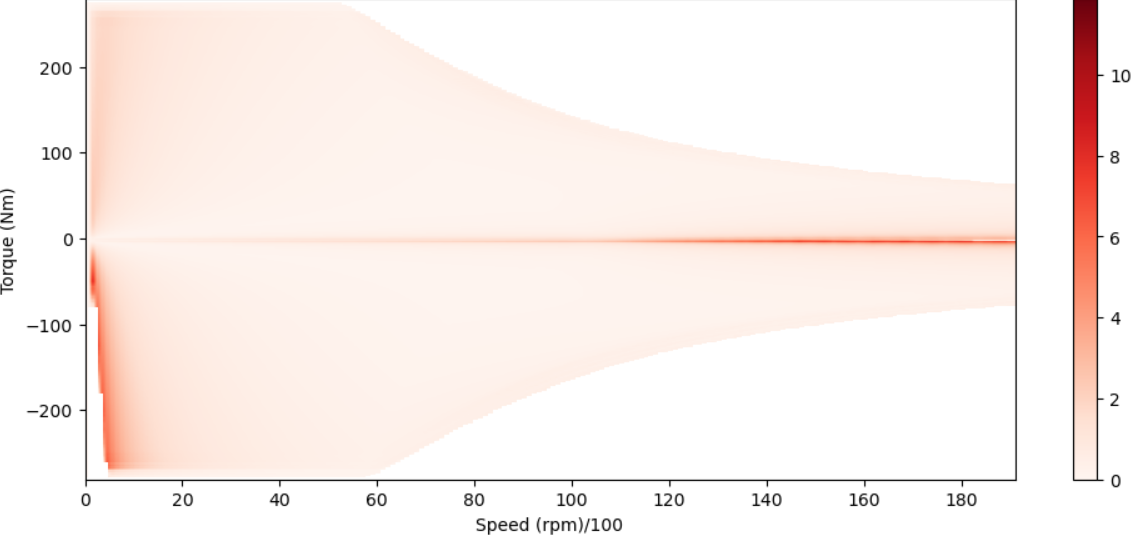
\includegraphics[width=0.75\textwidth]{./ReportImages/stddev_y2.png} 
    \caption{Standard Deviation of Efficiency \ac{KPI}} 
    \label{fig:Standard Deviation of 3D KPI(Efficiency)}
\end{figure}

\begin{figure}[H]
    \centering
    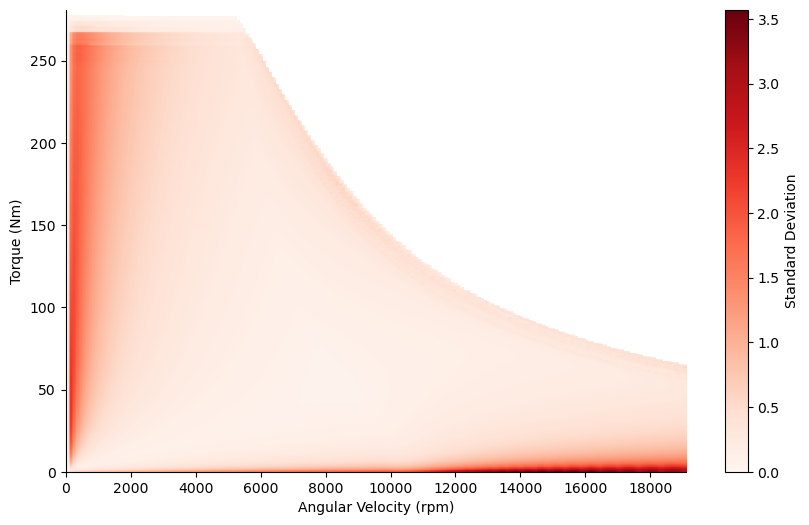
\includegraphics[width=0.75\textwidth]{./ReportImages/pos_stddev_y2.png} 
    \caption{Standard Deviation of Efficiency \ac{KPI} Positive Grid} 
    \label{fig:Standard Deviation of 3D KPI(Efficiency) Positive Grid}
\end{figure}

Figure \ref{fig:Standard Deviation of 3D KPI(Efficiency) Positive Grid across Angular Velocity Intervals} gives us the holistic view of how the efficiency values are 
distributed across equally spaced intervals of angular velocity. The Figure plots the standard deviation of all the Efficiency values of all samples of our dataset 
as an error bar for specific angular velocities at equal intervals of 2000 rpm.
The distributions shows maximum skewness towards extreme angular velocities and is relatively stable between 4000 and 6000 rpm. 
We discuss in Section \ref{sec:Loss for 3D KPI} how we integrate this finding into teaching over model.
Another assumption we can safely make is that the Efficiency grid for all samples look nearly alike. We arrive at this deduction by noting that standard deviation at its 
maximal is at 3. This gives us leverage to decide on choosing the Baseline model which will be further elaborated in Section \ref{sec:Results with Baseline}.

\begin{figure}[H]
    \centering
    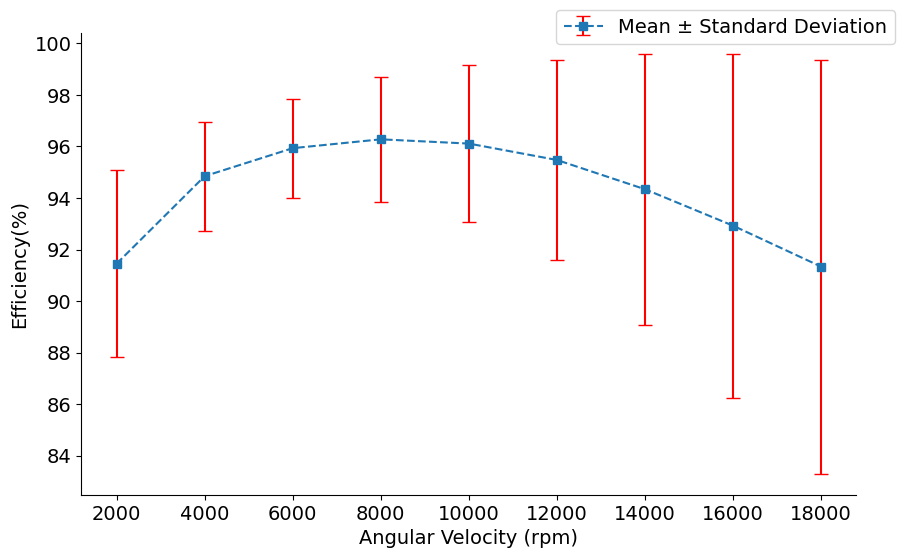
\includegraphics[width=0.8\textwidth]{./ReportImages/stddev_y2_nn_Target.png} 
    \caption{Standard Deviation of Efficiency \ac{KPI} Positive Grid across Angular Velocity Intervals} 
    \label{fig:Standard Deviation of 3D KPI(Efficiency) Positive Grid across Angular Velocity Intervals}
\end{figure}

Reading each sheet from the excel files particularlz the grids take up a lot of time and compute, hence we read the files as a onetime job when creating the 
tabular data for training  and store them into pythonic objects for faster access for training.
Both the input and target values for the Torque \ac{KPI} are stored locally as csv files whereas those of the Efficiency \ac{KPI} is stored as separate csv files per 
variant considering it is in the form of a 2\ac{D} array.
The csv files are then concatenated and stored into an array conserving dimensionality by padding \ac{NaN} values to match dimensionality of the grid 
corresponding to the Torque \ac{KPI} with the largest torque value.
In our case the value is 280 computed internally from the dataset but this is subject to change as we receive more data and there is a provision handy to override it 
on demand. The array is then saved locally for easy access and loading during training.

Initially we tried to set \ac{NaN} values as an incredibly high value hoping the model would consider this as a default value instead of \ac{NaN}.
However, it resulted in poor predictions as the model must have been confused and tried to increase its spread of predictions to cover this large value and so all 
true values were also predicted to be close to this dummy value.
Fortunately, we have come up with a better way of handling this scenario and we elaborate in Section \ref{sec:Loss for 3D KPI} how we tackle it.

\section{Scaling}\label{sec:Scaling}

Scaling is a common practice done before training a neural network. 
Standard scaling is the most prevalent scaling mechanism used for normalization as it results in a Gaussian Distribution centered around the mean.
We have used the same for the input features to bring them to a common scale. 

The Scaling is formulated mathematically as in Equation \ref{eq:Standard Scaling}
\begin{equation}
    \text{z} = \frac{x - \mu}{\sigma}
    \label{eq:Standard Scaling}
\end{equation} 
where $x$ is the Input, $\mu$ the Mean and $\sigma$ the Standard Deviation.
For the Input features both Mean and Standard deviation are calculated across columns. 
This is attributed to the fact we have columns with different ranges for the input since we consider each feature a column mentioned in Section \ref{subsec:Deep Dive into Input Parameters}.

We decided against scaling the targets owing to below 2 reasons :
\begin{enumerate}
    \item They do not enter the network architecture but are only used during loss calculation.
    \item If we scale the target we will have to scale each example from the train dataset and then average the calculated scaling parameters.
    % This in turn would mean 1 scaling parameter i.e, mean and standard deviation each for the entire dataset.
    It is not a good practice to do so as we will have lost a lot of originality in each example and is now introducing noise to new examples especially when they have a different data distribution.
    \item For the Efficiency \ac{KPI} we have loss regularization Equation \ref{eq:Y2 Maximum Efficiency Regularization} that has a constraint 
    check on the maximum range of efficiency values that can be predicted. If we had scaled the target, the constraint check would not be feasible to 
    implement as the maximum value that the constraint takes would also have to be scaled with the same scaler for comparison.
\end{enumerate}

During our experimentations where we initially scaled the targets, we observed then that the network required substantially less effort to learn and consequently lower learning rate and fewer epochs.
Since this comes at a tradeoff of losing precision, we continued with the original targets.

\section{Dataset splitting}\label{sec:Dataset splitting}
We convert the data to floating point tensors for better precision and collate them into a Tensor Dataset.
We have also partitioned the dataset to have about 50 samples for test and the remaining is used for 5 fold cross validation with 80:20 split for training and validation. 
The reason we have a separate test dataset from the validation is to ensure that there is no data leakage as we do not want to 
overfit the test dataset with the hyperparameters we choose during training. 
Across the 5 fold training runs, 4 sets would comprise of the training set and 1 of the test set which would be different for each fold run.
Therefore we expect to cover most grounds on training and have good monitoring on the model's performance for each fold.
Cross Validation also enables us to be able to monitor the network's overall stability and thus validate the model's generalization performance.
We have also used Data loaders to split the dataset into batches that fits into our \ac{GPU} memory.

\chapter{Modelling \& Evaluation}

For our multi regression problem, we train a \ac{MLP} on the tabular representation of the data.

\section{\ac{MLP} Model}\label{sec:MLP Model}

% \ac{MLP} is a feed forward network with no recurrent connections back to previous layers.
% The first layer of the network is the input layer, which distributes the input values to each neuron in the first hidden
% layer. The input values coming from the neurons of the previous layer has its own weights, and
% each hidden neuron has its own bias parameter. The weighted inputs and the bias are added up and the sum is fed for the input to activation function, which can be linear or nonlinear.
% The output of the activation function is then distributed to the next layers, or if the neuron is in the output layer, it is the model output

% the weights and biases are adjusted so that the model fits the training data

For the \ac{MLP} model, we use a single model with input features corresponding to all the features in the tabular topology invariant representation of the data.
The model architecture is build to predict both the Torque \ac{KPI} and Efficiency \ac{KPI}s by having 2 separate output layers for each of the \ac{KPI}s. 
Since the Torque \ac{KPI}'s targets are relatively learnable than that of the Efficiency \ac{KPI}'s targets we have experimented with fewer feed forward layers in the former than in the latter. \\
We have a hyperparameter to control the number of neurons in each hidden layer this can be tuned and is further discussed in Section \ref{tab:Hyperparameter Tunings}.
% A point of consideration is the hidden size for the shared layers and the MLP Torque layers cannot be varied much. This is further discussed in \ref{tab:Hyperparameter Tunings}.\\
\ac{ReLU} layers are also added in between to serve as the activation function and produce non-linearities and thus noise in the network. 
Dropout layers ensure that not all neurons in each layer are used up during training to prevent the model from memorizing the data and hence overfitting.  
We have 2 hyperparameters to control the dropout rate at which we freeze the neurons when training also to be discussed in Table \ref{tab:Hyperparameter Tunings}.
We use dropout for the shared layers of the \ac{MLP} and for the layers corresponding to Efficiency \ac{KPI}.
Batch normalization layers are used to normalize the input from the \ac{ReLU} activations applied on it and so mitigate internal co-variate shift to the next layer and hence speed up the training process.\\
Thus both batch normalization and dropout layers stabilize the network training.
Figure \ref{fig:MLP Model Architecture} gives an outline on how the \ac{MLP} Model architecture is designed. 
We discuss each component of the architecture below :
\begin{enumerate}
    \item \textbf{Input} \\
    The input layer takes in all features of the tabular data which is 89 in our case as scaled tensors.
    \item \textbf{MLP Shared} \\
    The MLP Shared block is a sequential block comprising of 2 Linear Layers with the input features and neurons of each hidden layer to be a hyperparameter we tune.
    We do not increase the number of neurons in the hidden layers within this block as it needs to be in the range of input features and output features(in this case Torque \ac{KPI}).
    Furthermore we have Batch Normalization layers between each linear and \ac{ReLU} activation function in addition to drop out layers.
    The dropout rate for the layers in this block is relatively higher as we want to encourage the model to focus largely on learning the generality of the data.
    The 2 Linear Layers enable the network to learn a rich representation of the data during the initial feature extraction phase.
    \item \textbf{MLP Torque} \\
    This block comprises of a Linear Layer with the output feature to be the size of the Torque \ac{KPI} and a \ac{ReLU} activation function.
    We use a \ac{ReLU} activation function at the end of the output as the target values are inherently always positive values and exploit \ac{ReLU}'s behavior of clipping negative values to 0.
    \item \textbf{MLP Efficiency} \\
    This block comprises of 3 Linear Layers with the output feature to be the size of the Efficiency \ac{KPI}.
    Here we also increase the neurons of the hidden layers as we are not limited by the dimensionality of the output feature.
    This would enable the model to be more strong and grasp the complex patterns in the data better.
    As usual we have batch normalization, dropout and \ac{ReLU} activation functions between the 1st two Linear layers.
    The dropout rate for the layers in this block is relatively lower as we want to encourage the model to learn the specific nature of the grid towards the end.
    For the Last Linear layer we have the output features corresponding to the target dimensions and a \ac{ReLU} activation again as the target values are inherently 
    always positive values and it again encourages the model to adhere to this fact.
    \item \textbf{Torque \ac{KPI}} \\
    The number of output features correspond to the target size 191 which is infact the range of angular velocities from 0 to 19000 rpm at equal spaced intervals of 2000rpm.
    Although the targets for the Torque \ac{KPI} are an array of integer values, we use the float tensor and not integer tensor to represent the data otherwise 
    it would become a classification problem and not a regression problem as it should be. 
    \item \textbf{Efficiency \ac{KPI}} \\
    The number of output features correspond to the target size which in our case is the shape of the padded collated array we had created in Section \ref{subsec:Deep Dive into 3D KPI}
\end{enumerate}

\begin{figure}[H]
    \centering
    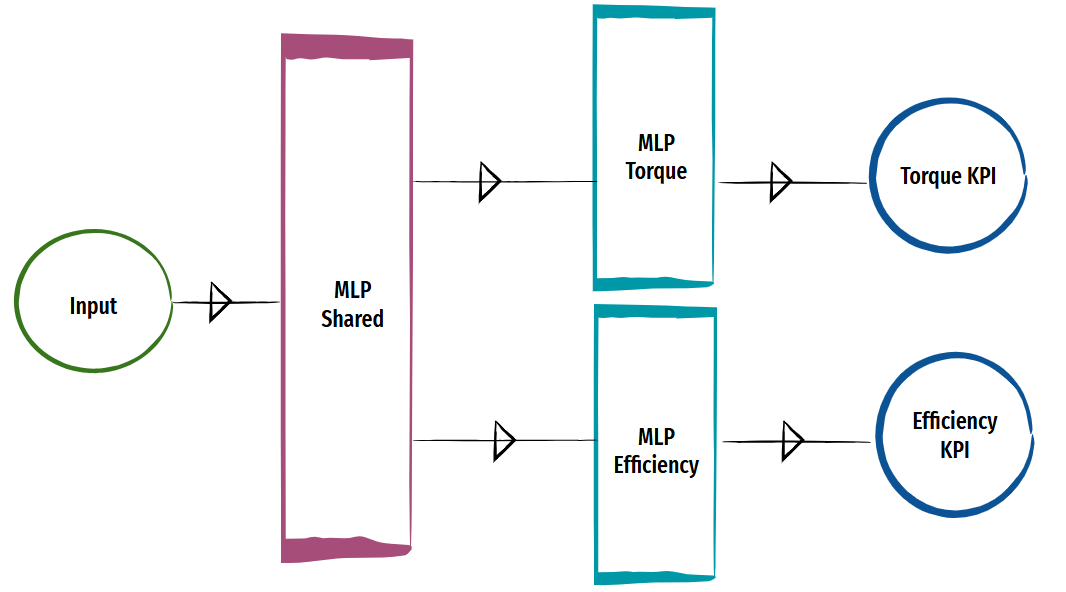
\includegraphics[width=0.8\textwidth]{./ReportImages/mlp_architecture.png} 
    \caption{MLP Model Architecture}
    \label{fig:MLP Model Architecture}
\end{figure}

\section{Loss Functions}\label{sec:Loss Functions}
The \ac{MSE} loss is the error metric used for our problem with the intention that the squared losses penalize the model and inturn encourage it to 
minimize the objective function even further. In addition to its contribution in exaggerating the loss by its square, \ac{MSE} also ensures that deviations are 
positive and do not confuse the model by negating the losses of opposing signs. 
\subsection{Loss for Torque \ac{KPI}(Torque curve)}\label{sec:Loss for 2D KPI}

The \ac{MSE} loss for the Torque \ac{KPI} is formulated mathematically as in Equation \ref{eq:Y1 Loss}
% Mean Squared Error (\ac{MSE}) Loss for 2D KPI
\begin{equation}
    \text{Y1 Loss} = \frac{1}{n} \sum_{i=1}^{n} \frac{1}{h} \sum_{j=1}^{h} (y_{ij} - \hat{y}_{ij})^2
    \label{eq:Y1 Loss}
\end{equation} 

where, \(n\) is \ac{EM} samples, \(h\) is the columns of the 1D Torque vector, \(y_{ij}\) and $\hat{y_{ij}}$ are the ij-th ground truth and prediction respectively for 
the torque at each operating point.

To encourage the model to learn the nature of the curve, we have experimented with 2 Loss Regularization techniques. 
Both of which are L2 Regularization to be in sync with the dynamics of the \ac{MSE} loss.
\begin{enumerate}
\item \textbf{Smoothening Loss Regularization} \\
To smoothen out the curve for the Torque \ac{KPI} we apply the below loss regularization factor to ensure that the torque values at neighboring operating points are 
as similar as possible. This is formulated mathematically as in Equation \ref{eq:Y1 Smoothening Loss Regularization}.
\begin{equation}
\text{Y1 Smoothening Loss Regularization} = \frac{1}{n} \sum_{i=1}^{n}\frac{1}{h-1} \sum_{j=1}^{h-1} \left(\sigma(|\hat{y}_{i{j+1}} - \hat{y}_{ij}| - 1)\right)^2 
\label{eq:Y1 Smoothening Loss Regularization}
\end{equation} 
where, $\sigma()$ is the \ac{ReLU} function.
This nature is factored in by penalizing the loss by the magnitude if the neighboring values in the prediction are not close to each other.
\ac{ReLU} helps to clips the difference if it is negative which is the scenario when a violation is not warranted.
\item \textbf{Decreasing Loss Regularization} \\
The Torque curve closely resembles a decreasing sigmoidal curve and hence we use this knowledge to penalize the loss for increasing consecutive values within the prediction. 
This is intended to ensure that the torque values making up th Torque curve at each operating point is less than or equal to its prior operating point.
This is formulated mathematically as in Equation \ref{eq:Y1 Declining Loss Regularization}.
\begin{equation}
    \text{Y1 Declining Loss Regularization} = \frac{1}{n} \sum_{i=1}^{n}\frac{1}{h-1} \sum_{j=1}^{h-1} \left(\sigma(\hat{y}_{i{j+1}} - \hat{y}_{ij})\right)^2
    \label{eq:Y1 Declining Loss Regularization}
\end{equation} 
It takes into consideration the almost continuous decreasing nature of the curve as the regularization is such that a specific element in the array is less than or 
equal to its prior element.
% If the electromagnetic coil is enabled by the commutator for the time span t3, the (almost) maximal current is running through it's loops and the (almost) maximal magnetic field strength is generated. The (almost) maximal torque is acting on the rotor. If the time span is shortened to t2 by increasing rotational speed, a slightly lower torque is acting, because the current through the coil is decreasing slightly. When reducing the time span to t1, the coil gets disconnected from the input voltage even though just half the maximum current is reached. Accordingly the torque decreases significantly:
%[https://homofaciens.de/technics-electric-motors-torque-curve_en.html]
% We add regularization term to help learn the parameters.
\end{enumerate}
We have not combined both the above regularizations as they donot complement each other. This is because the loss regularized by Equation 
\ref{eq:Y1 Smoothening Loss Regularization} will not necessarily be a decreasing curve.
This holds true for the regularization in Equation \ref{eq:Y1 Declining Loss Regularization} as it may not necessarily have gradual transitions in the curve.
Nevertheless, we perform ablation studies with both the regularizations and report the results obtained in Table \ref{tab:Ablation Studies}

\subsection{Loss for Efficiency \ac{KPI}(Efficiency Grid)}\label{sec:Loss for 3D KPI}

The \ac{MSE} loss for the Efficiency \ac{KPI} ca n be translated as in Equation \ref{eq:Y2 Loss}.
\begin{equation}
\text{Y2 Loss} = \frac{1}{n} \sum_{i=1}^{n} \frac{1}{w} \frac{1}{h} \sum_{j=1}^{w} \sum_{k=1}^{h} \left( M_{ijk} \cdot y_{ijk}) - (M_{ijk} \cdot \hat{y}_{ijk})\right)^2
\label{eq:Y2 Loss}
\end{equation}
\begin{equation}
    M_{ijk} = \begin{cases}
        1 & \text{if } y_{ijk} \neq \ac{NaN} \\
        0 & \text{if } y_{ijk} = \ac{NaN} 
        \end{cases} \\
\label{eq:Mask matrix}
\end{equation}
where, \(M_{ijk}\) is Mask matrix, \(w\) is the rows of 2\ac{D} vector and \(h\) the columns of 2\ac{D} vector.
% The Efficiency \ac{KPI} is a 3\ac{D} plot of real numbers representing percentage values and is always in the range of 0-100\%.\\
Based on one of our observation in Section \ref{subsec:Deep Dive into 3D KPI} on the efficiency values beyond the Efficiency envelope having blank values, 
which we had also padded them to be \ac{NaN} values we construct a binary mask matrix to ignore them in the loss calculation.
As ANN cannot be trained to predict \ac{NaN} values the binary mask is constructed such that values corresponding to \ac{NaN} in the target have value 0 and all other values as 1.
Mathematically, this process can be expressed as is in Equation \ref{eq:Mask matrix} and thus ensure that the \ac{NaN} values are ignored in the loss calculation. 
The mask is then multiplied with both the target and its respective prediction. 

We have also modelled 2 Loss Regularization techniques to encourage the model to learn the nature of the Efficiency \ac{KPI} curve.
\begin{enumerate}
\item \textbf{Maximum Efficiency Loss Regularization} \\
To ensure that the efficiency values do not exceed 100, we modify the objective functions mathematically as in Equation \ref{eq:Y2 Maximum Efficiency Regularization}.
\begin{equation}
\text{Y2 Maximum Efficiency Regularization} = \frac{1}{n} \sum_{i=1}^{n}\frac{1}{w} \frac{1}{h} \sum_{j=1}^{w} \sum_{k=1}^{h}\left(\sigma(|\hat{y}_{ijk}| - 100)\right)^2 
\label{eq:Y2 Maximum Efficiency Regularization}
\end{equation} 
\vspace{0.2cm} % Adjusts vertical space between equation and text
When the efficiency values of the prediction exceed 100, we penalize the overall loss by squared magnitude of the difference of the prediction from its ground truth.
\ac{ReLU} again assists to clips the difference if it is negative which is the scenario when the efficiency values are less than or equal to 100 when a violation is not warranted. \\
Needless to say the efficiency values are percentage values and can only take up values in the range of 0-100\%.
We refrain from instructing the model to not have values less than 0 since we mask \ac{NaN} values as 0 and the model will for sure attempt to predict values close to 0.
Moreover, these predictions are not relevant for us as after generating all predictions we finally slice off the Efficiency grid to be of the shape of the Torque curve 
which implies that the values predicted in place of \ac{NaN} are irrelevant. This is discussed more elaborately in Section \ref{sec:Post Processing}.
Therefore, we do not see the need to needlessly punish the model for making mistakes for values we eventually donot use as pessimistic decisions could discourage the model 
from realistic learning and thus affect its focus on predicting the other values in the Efficiency grid correctly.
\item \textbf{Efficiency Grid Loss Regularization} \\
Additionally, to encourage the model to learn the nature of the Efficiency \ac{KPI} from our observations gathered in Section \ref{subsec:Deep Dive into 3D KPI} and from 
the regions in Figure \ref{fig:Standard Deviation of 3D KPI(Efficiency) Positive Grid} which showed the most standard deviation, we have tried to incorporate all of 
the below learnings via the loss function as Y2 Regularization techniques.
\begin{enumerate}
\item \textbf{Efficiency at Maximum Torque Loss Regularization} \\
We cannot incorporate regularizing the loss to have the decreasing envelope of the Torque curve and so we only focus on what we can effectively teach the model which 
herein is the stable portion of the Torque curve typically until Angular Velocity of 5000 rpm. This is derived from an observation we make on the shape of the Torque 
curve in Section \ref{subsec:Deep Dive into 2D KPI}.
To ensure that the shape of the Efficiency \ac{KPI} is maintained, we also regularize the loss for the maximum torque value.
To do so, we have attempted to retrieve the last rows of our Efficiency \ac{KPI} and those of its target values and penalize the squared difference to have higher weight.
We formulate it mathematically as in Equation \ref{eq:Y2_Loss_Regularization_MM_Max_Torque}
\begin{equation}
    \text{Y2 Loss Regularization Max Torque} = \frac{1}{n} \sum_{i=1}^{n} \frac{1}{t_{1}} \sum_{j=-t_{1}}^{w} \frac{1}{h} \sum_{k=1}^{h} (y_{ijk} - \hat{y}_{ijk})^2
    \label{eq:Y2_Loss_Regularization_MM_Max_Torque}
\end{equation}
where, \(t_{1}\) is the threshold for initial Efficiency \ac{KPI} Envelope boundary. The number of last rows is determined by a threshold $t_{1}$.
The intention of including the threshold value is to give the model the flexibility to search a certain portion of the Efficiency grid determined by the threshold and 
push the model to get this region right by having 0s for values in prediction but not in target.
\item \textbf{Efficiency at Low Angular Velocity Loss Regularization} \\
It is a known fact that at Torque 0 Nm, the corresponding efficiency values for the motor is 0\%. Consequently the efficiency values close to this torque will be low.
To force the model to pay more attention at lower angular velocities, we have regularized the loss for the first few columns of each row of the predicted Efficiency grid 
and penalize the squared difference with that of its target. We formularize it mathematically as in Equation \ref{eq:Y2_Loss_Regularization_Low_Speed}:
\begin{equation}
    \text{Y2 Loss Regularization Low Angular Velocity} = \frac{1}{n} \sum_{i=1}^{n} \frac{1}{w} \sum_{j=1}^{w} \frac{1}{t_{2}} \sum_{k=1}^{t_{2}} (y_{ijk} - \hat{y}_{ijk})^2
    \label{eq:Y2_Loss_Regularization_Low_Speed}
\end{equation}
where, \(t_{2}\) is the Threshold for Low Angular Velocities. The number of first columns is determined $t_{2}$. 
The intention of including the threshold value here is to give the model the flexibility to search the relevant portion of the Efficiency grid determined by the threshold 
and push the model to get the region of low angular velocities right by penalizing this region more.
\item \textbf{Efficiency at Low Torque Loss Regularization} \\
At extreme speeds we find a greater deviation in the efficiency values particularly towards higher speeds. This is because we have fewer efficiency values as speed 
increases beyond a range since not all torque values participate.
To force the model to be more careful at low torque, we have regularized the loss for the first few rows of each column of the Efficiency \ac{KPI} and penalize the 
squared difference with that of the target. 
We formulate it mathematically as in Equation \ref{eq:Y2_Loss_Regularization_Low_Torque}:
\begin{equation}
    \text{Y2 Loss Regularization Low Torque} = \frac{1}{n} \sum_{i=1}^{n} \frac{1}{t_{3}} \sum_{j=1}^{t_{3}} \frac{1}{h} \sum_{k=1}^{h} (y_{ijk} - \hat{y}_{ijk})^2
    \label{eq:Y2_Loss_Regularization_Low_Torque}
\end{equation}
where, \(t_{3}\) is the Threshold for Low Torque. The number of first rows is determined by $t_{3}$.
The intention of including the threshold value herein is to give the model the flexibility to search the relevant portion of the Efficiency grid determined by the threshold 
and push the model to get the regions of low Torques right by penalizing this region more.

The above Y2 Regularizations are indeed purely \ac{MSE} but with higher weights for specific regions of the Efficiency \ac{KPI}.
Consequently being L2 Regularizations it goes hand in hand with \ac{MSE} Loss calculated in Equation \ref{eq:Y2 Loss}.
The thresholds \(t_{1}\),\(t_{2}\) and \(t_{3}\) are tunable hyperparameters that we can optimize if we observe the relevant ports of the Efficiency \ac{KPI}'s visualization 
not adhering to the expected look of the Efficiency grid.
We aggregate all the above regularizations to form the Y2 Loss Regularization as in Equation \ref{eq:Y2 Efficiency Grid Loss Regularization}
\begin{equation}
    \begin{split}
    \text{Y2 Efficiency Grid Loss Regularization} = \text{Y2 Loss Regularization Max Torque} \\
    + \text{Y2 Loss Regularization Low Angular Velocity} + \text{Y2 Loss Regularization Low Torque}
    \end{split}
    \label{eq:Y2 Efficiency Grid Loss Regularization}
\end{equation}
\end{enumerate}
\end{enumerate}

The Total Loss is calculated in Equation \ref{eq:Total Loss}
\begin{equation}
    \begin{split}
\text{Total Loss} = \text{wt} \times (\text{Y1 Loss} + (\lambda_{\text{1y1}} \times \text{Y1 Smoothening Loss Regularization}) +  (\lambda_{\text{2y1}} \times \\
\text{Y1 Declining Loss Regularization })) + \text{(1-wt)} \times ((\text{Y2 Loss} + (\lambda_{\text{y21}} \times \\ 
\text{Y2 Maximum Efficiency Loss Regularization}) + (\lambda_{\text{y22}} \times \\
\text{Y2 Efficiency Grid Loss Regularization})))
    \end{split}
    \label{eq:Total Loss}
\end{equation}
where, \(\lambda_{\text{1y1}}\) is Y1 Smoothening Loss Regularization Parameter, \(\lambda_{\text{2y1}}\) is Y1 Declining Loss Regularization Parameter,
        \(\lambda_{\text{y21}}\) is Y2 Maximum Efficiency Loss Regularization Parameter, \(\lambda_{\text{y21}}\) is Y2 Efficiency Grid Loss Regularization Parameter, 
        \(wt\) is Y1 Loss Weightage, \(1-wt\) is Y2 Loss Weightage. \\

We have added a Weightage parameter that controls the contribution of the Y1 Loss and Y2 Loss to the Total Loss. There are 2 reasons why this is useful for us :
\begin{enumerate}
    \item  When the targets are not of the same scale. \\
    Without scaling, the losses for both targets Torque and Efficiency \ac{KPI}s being of different ranges are drastically different.\\
    We circumvent this by weighing up the loss of the target not performing better on validation dataset and weighing down the loss of the 
    targets by the factor of how much its value range varies.
    \item When the prediction accuracy of one \ac{KPI} is substantially more vital than the other. 
    Our task demands the same as the Efficiency \ac{KPI} is post processed to be within the shape of the Torque \ac{KPI}. \\
    Therefore, in theory have higher weightage for the Torque \ac{KPI} as its loss in performing well is costlier but as its value range is relatively higher we make decisions from monitoring the perdiction performances.\\
    We reflect on these decisions based on whether the envelope of the Efficiency \ac{KPI} grid is more valuable that the efficiency values within it.\\
    To counter the Torque \ac{KPI} loss dominating the total loss, we have implemented quite a few regularization techniques to the Efficiency \ac{KPI} loss.\\
    Ultimately we decided on prioritizing the efficiency values.
\end{enumerate}
Furthermore, the weightage parameters for both target is designed to sum upto 1 keeping in mind improved training stability as a result of normalized weights. \\
Finally the aggregated loss is backpropagated.

\section{Optimizer}\label{sec:Optimizer}

Adam optimizer is used for optimization as it is known to be computationally efficient and requires less memory \cite{ADAM-2017}. \\
It infers the gradients of the loss and how it impacts the weights and biases of each layer and thus controls learning by guiding the model to decrease the loss over the course of training. \\
The optimizer acts once the loss is backpropagated across training each batch of the dataset.\\
The optimizer also uses the learning rate to control the step size with which the model parameters are updated.\\

\section{Evaluation Metrics}
The evaluation metrics we have considered for our regression problem is the average of the \ac{RMSE}. \\
Therefore, the model with the least prediction scores ie, closest to 0 is ideal for our application. \\

\subsection{Evaluation Metrics for Torque \ac{KPI}}\label{sec:Evaluation Metrics for 2D KPI}
The Y1 Score for the Torque \ac{KPI} is formulated in Equation \ref{eq:Y1 Score} :
\begin{equation}
\text{Y1 score} = \frac{1}{n} \sum_{i=1}^{n} \underbrace{ \sqrt{\frac{1}{h} \sum_{j=1}^{h} (y_{ij} - \hat{y}_{ij})^2}}_{Y1\ RMSE}
\label{eq:Y1 Score}
\end{equation}
where, \(h\) is the columns of 1D vector and \(Y1\ \ac{RMSE}\) is \ac{RMSE} for each test sample.

\subsection{Evaluation Metrics for Efficiency \ac{KPI}}\label{sec:Evaluation Metrics for 3D KPI}
The Y2 score for the Efficiency \ac{KPI} is formulated in Equation \ref{eq:Y2 Score} :
\begin{equation}
    \text{Y2 score} = \frac{1}{n} \sum_{i=1}^{n} \underbrace{ \sqrt{\frac{1}{w} \frac{1}{h} \sum_{j=1}^{w} \sum_{k=1}^{h} (y_{ijk} - \hat{y}_{ijk})^2}}_{Y2\ RMSE}
    \label{eq:Y2 Score}
\end{equation}
where, \(w\) is the rows of 2\ac{D} vector, \(h\) is columns of 2\ac{D} vector and \(Y2\ \ac{RMSE}\) is the \ac{RMSE} for each test sample.

\section{Post Processing}\label{sec:Post Processing}
The mean and standard deviation from the train-validation datasets are applied to transform the test dataset to maintain uniformity in the predictions generated.
In the case of new files not part of the segregated test dataset we first convert it into the tabular representation our model consumes and then apply the scaling.\\
This is why we preserve the same scalers used during training as we not only evaluate our dedicated test dataset but also for clients to use on demand. 

Furthermore as we are predicting a padded matrix to ensure dimensionality sync across different Efficiency \ac{KPI}s, the grid contains values even outside the boundary of the Efficiency \ac{KPI}.
First we tried to slice of the grid to ignore 0 values for all rows excluding the 1st row as per the Equation \ref{eq:Y2_Loss_Regularization_Low_Speed}.
We hoped the Mask constructed from equation \ref{eq:Mask matrix} would force the model to learn 0s for however it tried to approximate close to 0 and was almost never 0.
Hence, we decided to slice the shape of the Torque \ac{KPI} curve from the Efficiency \ac{KPI} by counting the number of columns a row to have based on consecutive values in the curve.
This brings us back to the point that it is imperative the prediction of the Torque \ac{KPI} is close to perfect as the envelope of the Efficiency \ac{KPI} inherently is dependent on it.
However if in the worst case scenario where the y1 and y2 predictions are so starkly different that Efficiency \ac{KPI} cannot be sliced off from 
the Torque \ac{KPI} because the former is smaller than the latter then we decide not to slice the Efficiency \ac{KPI} and instead use the predictions as is.

\newpage 
\newpage 

% Masking NaN values
\chapter{Experiments and Results}

\section{Experiments with \ac{MLP}}\label{sec:Experiments with MLP}

After optimizing over an exhaustive random search of the hyperparameter space, we present them in Table \ref{tab:Hyperparameter Tunings} by monitoring the model's 
performance across 5 fold cross validation. We use different splits for each round of training and tune the hyperparameters on the validation set. 
The final splits are saved locally and can be used later to ensure reproducibility. 

\begin{table}[H]
    \centering
    % \begin{tabularx}{1\linewidth}{|X|X|X|X|}
    \begin{tabularx}{\linewidth}{|p{0.625\textwidth}|p{0.15\textwidth}|p{0.145\textwidth}|}
    \hline {\bf Hyperparameters} & {\bf Value} & {\bf Value Ranges}\\
    \hline 
    Learning Rate (lr) & 0.075 & 0.025 - 0.25\\
    Dimensionality of Hidden Layers (hidden size)& 128 & 64, 128\\
    Exponential Learning Rate Scheduler Gamma Parameter (lr gamma)& 0.9 & 0.5-0.9\\
    Batch Size (batch size)& 72 & 32-72\\
    Number of Epochs (epochs)& 10 & 6-10\\
    Dropout Probability for Shared Layers ($p_{y1}$)& 0.35 & 0.4-0.2\\
    Dropout Probability for Efficiency Layers ($p_{y2}$) & 0.2 & 0.2-0.1\\
    Y1 Smoothening Curve Loss Regularizer ($\lambda_{1y1}$) & 0.5 & 0-0.75\\
    Y1 Decreasing Curve Loss Regularizer ($\lambda_{2y1}$)& 0.5 & 0-0.75\\
    Y2 Maximum Efficiency Value Regularizer ($\lambda_{y21}$) & 5 & 0-5\\
    Y2 Efficiency Grid Loss Regularizer ($\lambda_{y22}$) & 3.75 & 0-5\\
    Y2 Initial Envelope Boundary Threshold ($t_{1})$& 5 & 0-5\\
    Y2 Low Speed Threshold ($t_{2}$)& 20 & 0-30\\
    Y2 Low Torque Threshold ($t_{3}$)& 20 & 0-30\\
    Weightage of Y1 Loss (wt)& 0.05 & 0-1\\
    Weightage of Y2 Loss (1-wt)& 0.95 & 0-1\\
    \hline
    \end{tabularx}
    \caption{Hyperparameter Tuning}
    \label{tab:Hyperparameter Tunings}
\end{table}

We are using a learning rate scheduler which reduces the learning rate exponentially by the \textit{lr gamma} to decay learning as training progresses across epochs.
This is to ensure that the model does not overshoot after few cycles of training.
The \textit{batch size} is limited to the capacity of our \ac{GPU} memory. We use the maximum batch size to train faster and therefore use 72 after which we hit the 
memory roof of our GPU.
The \textit{hidden size} refers to the number of neurons in the hidden layers of the \ac{MLP} model. We have experimented with just 2 hidden sizes as we are 
constrained by the fact that the number of neurons must be between the range of input features and output features which was discussed in Section \ref{sec:MLP Model}.
In addition it has to be of the multiples of 8 as \ac{GPU}s are most optimized for the same.
Dropout rate during training is controlled by the parameter \textit{$p_{y1}$} for shared layers and \textit{$p_{y2}$} for layers specific to Efficiency \ac{KPI}. 
This is discussed in Section \ref{sec:MLP Model}. We are not so much concerned of the data being dropped in larger extent than anticipated for the Torque \ac{KPI} 
because it is relatively simpler to learn and the value range is comparatively larger leading its loss to dominate the total loss.
\textit{$\lambda_{1y1}$}, \textit{$\lambda_{2y1}$}, \textit{$\lambda_{y21}$} and \textit{$\lambda_{y22}$} parameters control the regularization weight for the 
regularization terms for the Torque \ac{KPI} and Efficiency \ac{KPI} respectively detailed in Equation \ref{eq:Total Loss}.
The thresholds \textit{$t_{1}$}, \textit{$t_{2}$} and \textit{$t_{3}$} are used to control the number of rows and/or columns to be considered for the loss
regularization terms to learn the nature of the Efficiency \ac{KPI} as detailed in Section \ref{sec:Loss for 3D KPI}.
The weightage parameter to control the direction of loss is denoted by \textit{wt} and is also discussed in Equation \ref{eq:Total Loss}.

We also observe that a simple architecture of the model is not a significant downside for limited data set as it seems to learn the patterns within the data 
especially since we supplement the loss regularization with more knowledge.
Our main \ac{MLP} model only uses the loss regularization parameters \textit{$\lambda_{2y1}$} and \textit{$\lambda_{y2}$} ie, it does not consider the Smoothing curve 
regularization for the Torque \ac{KPI} whose performance we will separately discuss in Section \ref{sec:Ablation Studies}.

We chose a 3rd party application \texttt{Wandb}\footnote{Weights \& Biases} to log metrics from the training run and to monitor model performance across the 5 folds.
All 5 folds are monitored and shown in the Figures as training and validation occurs 5 times on different combinations of cross validation splits independent per fold.

Figure \ref{fig:Training Loss Metrics} illustrates the loss at work as training progresses across epochs. 
Figures \ref{fig:Training Loss Metrics} \ref{sub@fig:Training Loss for Torque Curve} and \ref{fig:Training Loss Metrics} \ref{sub@fig:Training Loss for Efficiency grid} 
provides monitoring of how the losses for both the \ac{KPI}s vary. As was discussed in Equation \ref{eq:Y1 Loss} and Equation \ref{eq:Y2 Loss}, both the \ac{MSE} losses 
also include their respective loss regularization terms weighted by the tunable regularization coefficients. 
Figure \ref{fig:Training Loss Metrics} \ref{sub@fig:Aggregated Training Loss} depicts the weighted sum of losses 
discussed in Equation \ref{eq:Total Loss}.

\begin{figure}[H]
    \centering
    \begin{subfigure}{0.32\textwidth}
        \centering
        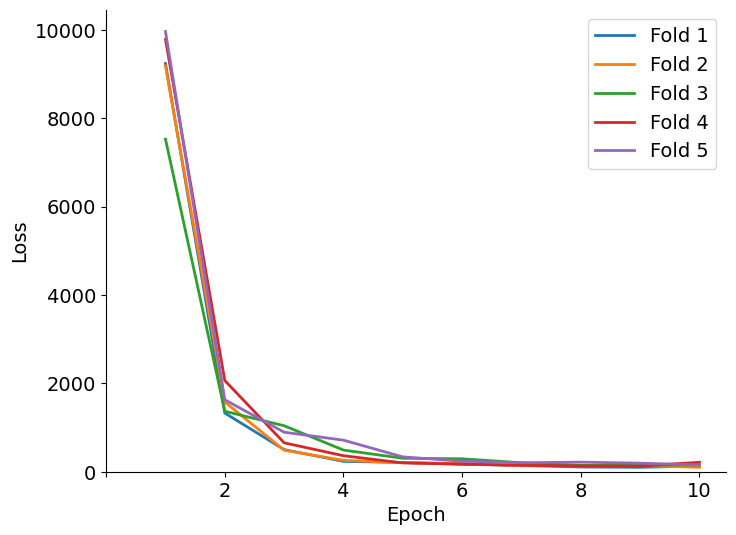
\includegraphics[width=\textwidth]{./ReportImages/train_loss.png}
        \caption{\centering Aggregated Training Loss}
        \label{fig:Aggregated Training Loss}
    \end{subfigure}\hfill
    \begin{subfigure}{0.32\textwidth}
        \centering
        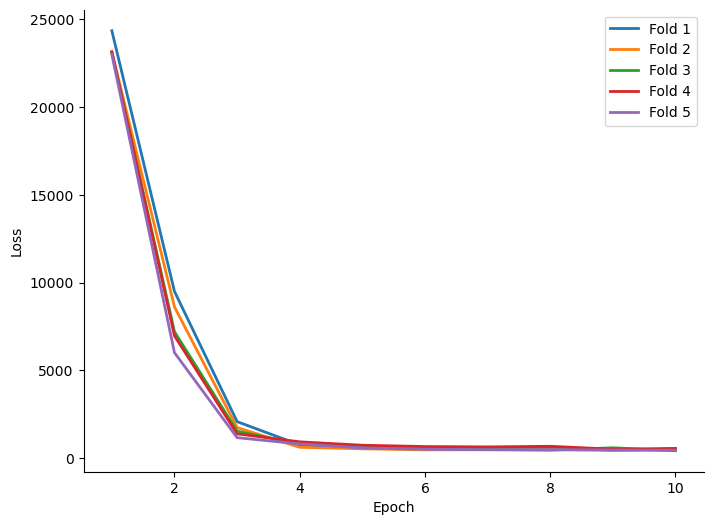
\includegraphics[width=\textwidth]{./ReportImages/train_loss_y1.png}
        \caption{\centering Training Loss for Torque \ac{KPI}}
        \label{fig:Training Loss for Torque Curve}
    \end{subfigure}\hfill
    \begin{subfigure}{0.32\textwidth}
        \centering
        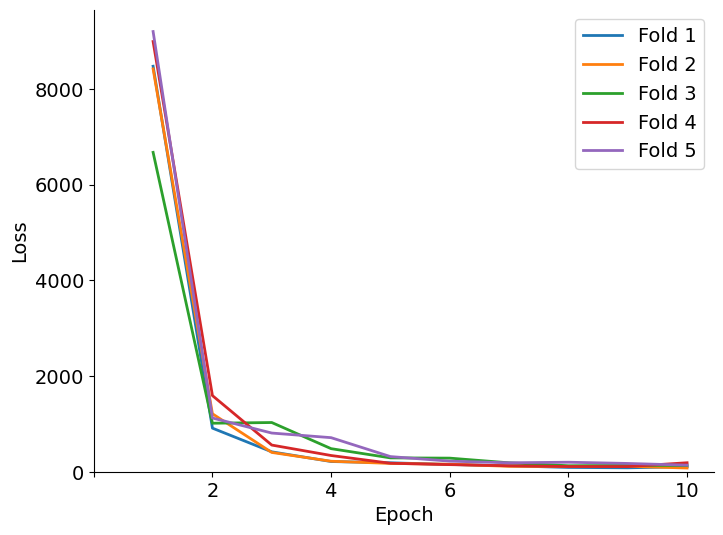
\includegraphics[width=\textwidth]{./ReportImages/train_loss_y2.png}
        \caption{\centering Training Loss for Efficiency \ac{KPI}}
        \label{fig:Training Loss for Efficiency grid}
    \end{subfigure}
    \caption{Training Loss Metrics}
    \label{fig:Training Loss Metrics}
\end{figure}

From the training plots we see that the model has converged after having run for 10 epochs with a total run time of 3 MNIUTES VERIFY:
Even though the weightage assigned to the Efficiency \ac{KPI} is significantly more in addition to loss regularization parameter, it seems to have stopped learning 
beyond a threshold and so we hypothesize to further increase the weightage of the Efficiency \ac{KPI}.
The Torque \ac{KPI} shows promise in learning better but it would be at the cost of overfitting the Efficiency \ac{KPI}.
\begin{figure}[H]
    \centering
    \begin{subfigure}{0.32\textwidth}
        \centering
        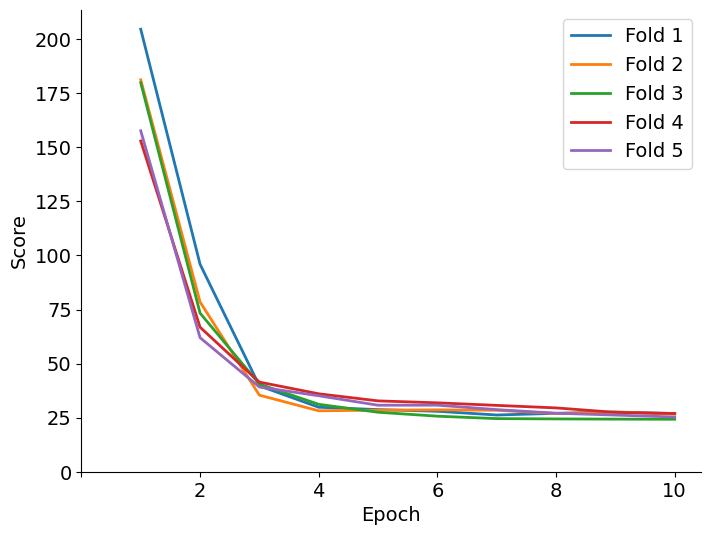
\includegraphics[width=\textwidth]{./ReportImages/val_score.png}
        \caption{\centering Aggregated Validation Score}
        \label{fig:Aggregated Validation Score}
    \end{subfigure}\hfill
    \begin{subfigure}{0.32\textwidth}
        \centering
        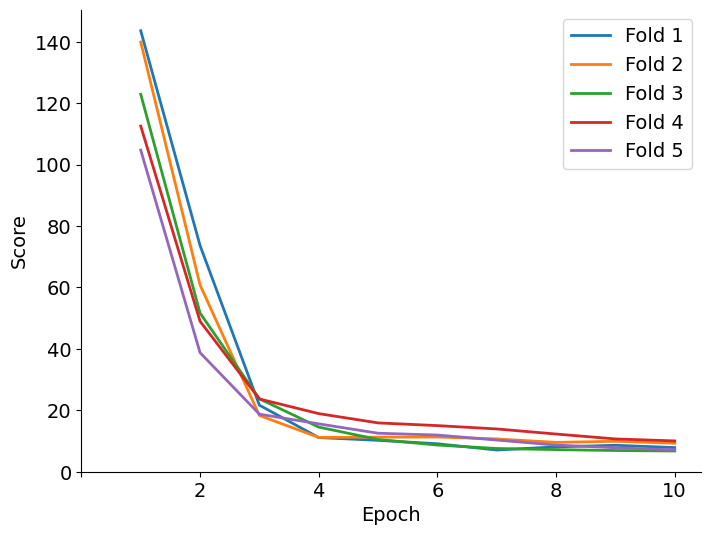
\includegraphics[width=\textwidth]{./ReportImages/val_score_y1.png}
        \caption{\centering Validation Score for Torque \ac{KPI}}
        \label{fig:Validation Score for Torque Curve}
    \end{subfigure}\hfill
    \begin{subfigure}{0.32\textwidth}
        \centering
        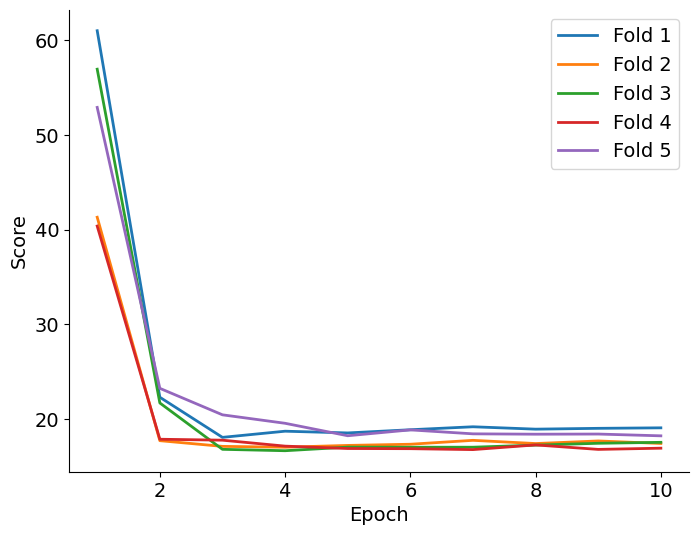
\includegraphics[width=\textwidth]{./ReportImages/val_score_y2.png}
        \caption{\centering Validation Score for Efficiency \ac{KPI}}
        \label{fig:Validation Score for Efficiency grid}
    \end{subfigure}
    \caption{Validation Evaluation Metrics}
    \label{fig:Validation Evaluation Metrics}
\end{figure} 

The Validations plots for losses also tells us the same tale although the Efficiency \ac{KPI} stops to learn after a certain point can be monitored in \ref{fig:Validation Loss Metrics}.
Figure \ref{fig:Validation Evaluation Metrics} illustrates the evaluation metrics changing across each epoch of the validation dataset. This is important to us to know 
the model's performance on unseen data fot the 5 folds. Figure \ref{sub@fig:Aggregated Validation Score} shows the aggregated validation score which is again the weighted 
sum of the scores as was formulated in Equation CITE for both the \ac{KPI}s displayed in Figure \ref{sub@fig:Validation Loss for Torque Curve} and Figure 
\ref{sub@fig:Validation Score for Efficiency grid} respectively. Likewise the training plots evaluation metrics are displayed in Figure \ref{fig:Training Evaluation Metrics}.

The training loss and validation evaluation plots are most important to us to be able to judge the hyperparameters to optimize. 
Therefore the other plots are moved to Appendix \ref{sec:Experimental setup} for further reflection.

Our observations from the validation plots are : LIST THEM

We have also enabled saving the best performant fold locally so it can be loaded on demand by the client when in need to only run inference.\\
As the value ranges for both the \ac{KPI}s are starkly different, we give a glimpse of the percentage difference
We have narrowed down scoring to follow the criteria as recorded in Table \ref{tab:Scoring Criteria}.
\begin{table}[H]
    \centering
    \begin{tabularx}{1\linewidth}{|X|X|X|X|X|X|X|X|X|X|}
    \hline {\bf \% Difference} & {\bf 0-5\%} & {\bf 5-10\%} & {\bf 10-15\%} & {\bf 15-20\%} & {\bf 20-25\%} & {\bf 25-30\%} & {\bf 30-35\%} & {\bf 35-40\%} & {\bf 40-100\%}\\
    \hline 
    Y1 Score& 0-11& 11-22 & 22-33 & 33-44 & 44-55& 55-66 & 66-77 & 77-88 & \textgreater 88\\
    Y2 Score& 0-5 & 5-10 & 10-15 & 15-20 & 20-25& 25-30 & 30-35 & 35-40 &\textgreater 40\\
    \hline
    \end{tabularx}
    \caption{Scoring Criteria}
    \label{tab:Scoring Criteria}
\end{table}

This is deduced from the Equations \ref{eq:Y1 Percentage Difference} and \ref{eq:Y2 Percentage Difference}.
\begin{equation}
    \text{Y1 Percentage Difference} = (\text{Y1 Score} / {(Y1 Max - Y1 Min)})  \times 100
    \label{eq:Y1 Percentage Difference}
\end{equation}
\begin{equation}
    \text{Y2 Percentage Difference} = (\text{Y2 Score} / {(Y2 Max - Y2 Min)})  \times 100
    \label{eq:Y2 Percentage Difference}
\end{equation}

From our observations the target values for Torque \ac{KPI} range between 50-280 and those of the Efficiency \ac{KPI} range between 0-100.
The scoring of the Y2 at inference is slightly different from that of training in the sense that for inference, we have the Torque \ac{KPI} to 
accurately slice of the envelope from the Efficiency \ac{KPI}. Also need to ensure how the difference works for NAN especially at inference coz 
for Training there are no NANs and in targets it would be 0. But for training, we cant slice the envelope as we dont have the Torque curve yet.--TO BE REMMOVED

\section{Results with \ac{MLP}}\label{sec:Results with MLP}
\subsection{Torque \ac{KPI} Results with \ac{MLP}}\label{sec:2D Torque Curve Results with MLP}

\begin{figure}[H]
    \centering
    \includegraphics[width=1\textwidth]{./ReportImages/KPI2D_predictions.png} 
    \caption{MLP Training Results for Torque \ac{KPI}} 
    \label{fig:MLP Training Results for 2D KPI(Torque)}
\end{figure}

Figure \ref{fig:MLP Training Results for 2D KPI(Torque)} illustrates 6 test dataset predicted Torque values and their corresponding ground truths displayed against their angular velocities.
The torque values are only displayed for the range of torque participating in the Torque curves and so the continuity to 0 Nm is not maintained here to ensure effective space 
utilization. We also depict the difference and percentage difference on a twin y axis to give a rough overview of the prediction deviations from the targets.
As the percentage difference formulated in Equation \ref{eq:Y1 Percentage Difference} would always result in positive values, they appear above the 0 line dotted separator.+
Although we do see deviations, we notice for most of the cases, the predictions are such that the torque values predicted have smaller values than its respective ground truths.
In addition, the \ac{RMSE} equivalent to the Y1 score tells us that for 50\% of the plots shown, the predictions are off by about 5\% from the target values as per 
Table \ref{tab:Scoring Criteria}.

Figure \ref{fig:MLP RMSE Evaluation for 2D KPI(Torque)} shows us the Average \ac{RMSE} and element wise \ac{RMSE} for the test dataset performance with the \ac{MLP}. 
This figure closely resembles the skeleton of the Figure \ref{fig:Standard Deviation of 2D KPI} in terms of what is displayed. The only difference we can highlight is 
that the \ac{RMSE} with that of the ground truth is plotted instead of standard deviation on the twin y-axis in red.
Overall our inferences are the predictions closely resemble the trajectory of the target values although they fluctuate. Experimenting with the hyperparameters 
\textit{$\lambda_{1y1}$} and \textit{$\lambda_{2y1}$} has potential to improve this anomaly. In addition, granting a higher weight \textit{wt} can also help in this direction.

\begin{figure}[H]
    \centering
    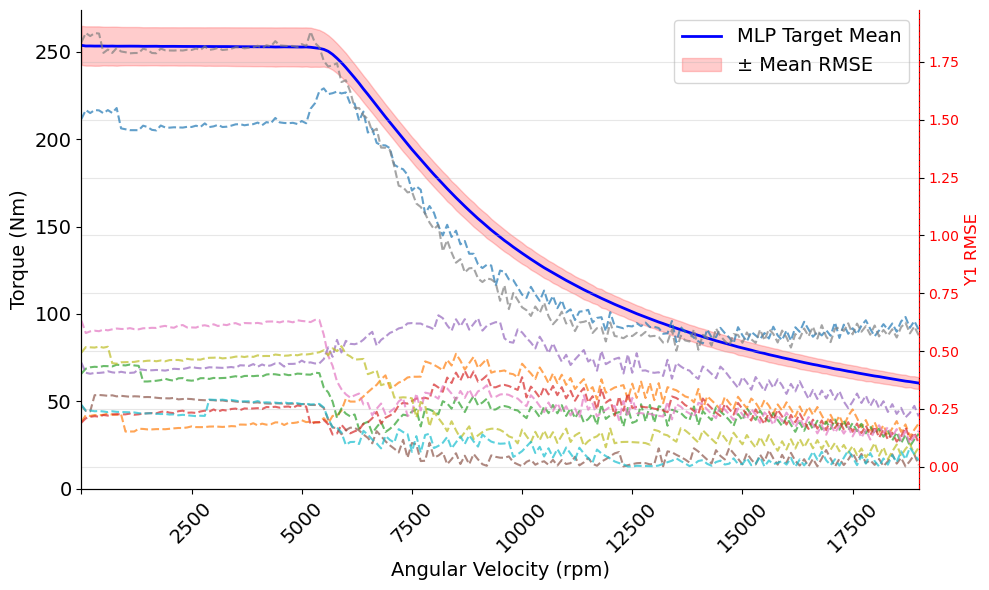
\includegraphics[width=0.75\textwidth]{./ReportImages/RMSE_MLP_y1.png} 
    \caption{\ac{MLP} \ac{RMSE} Evaluation for Torque \ac{KPI}} 
    \label{fig:MLP RMSE Evaluation for 2D KPI(Torque)}
\end{figure}

Figure \ref{fig:Y1 Evaluation Statistics MLP} shows the score statistics of the model performance of Torque \ac{KPI} over few samples from the test dataset 
with the number of test dataset samples on the y-axis.
The Y1 \ac{RMSE} from Equation \ref{eq:Y1 Score} is calculated for each sample and shown as a histogram in Figure \ref{fig:Y1 RMSE}.
The Y1 Percentage Difference from Equation \ref{eq:Y1 Percentage Difference} is calculated for each sample and shown as a histogram in Figure 
\ref{fig:Y1 Evaluation Statistics MLP}, this is essential to be able to relate to its effect on total range of deviation due to its differing value range. 
The histogram looks the same in shape for both the figures however the finer details lies within the measure on the x-axis.

\begin{figure}[H]
    \centering
    \begin{subfigure}{0.5\textwidth}
        \centering
        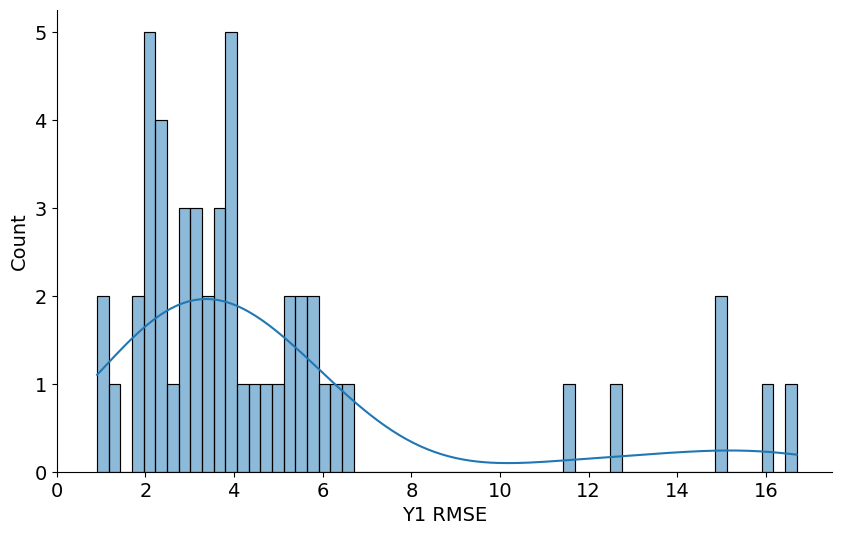
\includegraphics[width=\textwidth]{./ReportImages/score_MLP_y1.png}
        \caption{Y1 \ac{RMSE}}
        \label{fig:Y1 RMSE}
    \end{subfigure}\hfill
    \begin{subfigure}{0.5\textwidth}
        \centering
        \includegraphics[width=\textwidth]{./ReportImages/percentage_diff_MLP_y1.png}
        \caption{Y1 Percentage Difference}
        \label{fig:Y1 Percentage Difference}
    \end{subfigure}
    \caption{Y1 Evaluation Statistics of \ac{MLP}}
    \label{fig:Y1 Evaluation Statistics MLP}
\end{figure}

The observation we can deduce is that the \ac{RMSE}s are almost evenly distributed between 0.5-12.5 thus encompassing a range of 0-6\% difference with the target values.

\begin{figure}[H]
    \centering
    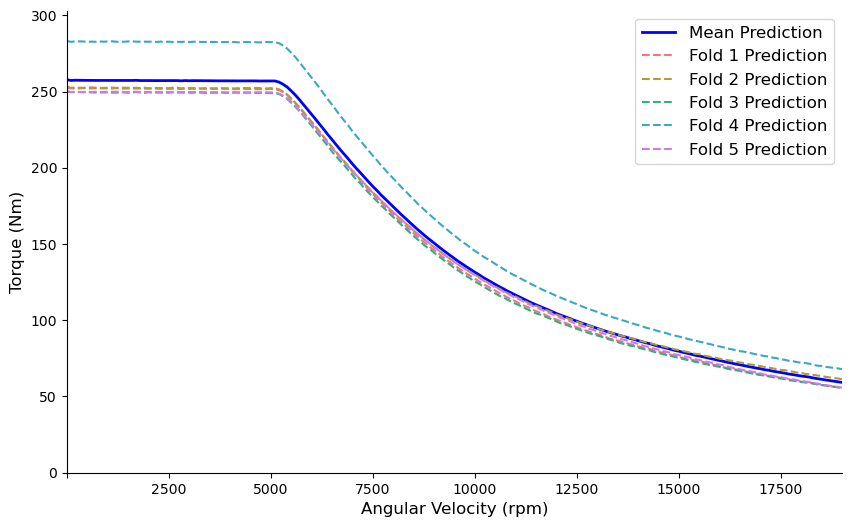
\includegraphics[width=0.6\textwidth]{./ReportImages/folds_dev_y1.png} 
    \caption{MLP Training Deviation across Folds for Torque \ac{KPI}} 
    \label{fig:MLP Training Deviation across Folds for Torque KPI}
\end{figure}

Figure \ref{fig:MLP Training Deviation across Folds for Torque KPI} gives a good view of how the torque curve for each folds prediction represented in dotted lines deviate 
from the mean of all the folds predicted torque curve. We can observe that each predicted torque curve is as close as can be to the mean of all the folds torque curves.
This figure is a good indicator of the model's generalization capability and also sheds light to the model's stability.
We also take care to note that we have used only 1 sample from the test dataset for inference across all folds.
A noteworthy point is that we have left the output predictions for the Torque curve to remain as floating point values even when the target values are integers 
to preserve data precision. We give the client the flexibility to turn this on/off demand.

\subsection{Efficiency \ac{KPI} Results with \ac{MLP}}\label{sec:3D Efficiency Grid Results with MLP}
Figure \ref{fig:Efficiency KPI Predictions Vs Targets with MLP} shows 3 sample predictions of the Efficiency \ac{KPI} from the test dataset alongside its ground truth.
Torque is displayed against its angular velocities and all efficiency values within the envelope can be viewed as differing colors in a contour plot. 
The figures are augmented with a scale showing the efficiency values in percentage across varying levels.

\begin{figure}[H]
    \centering
    \begin{subfigure}{1\textwidth}
        \centering
        \includegraphics[width=1\textwidth]{./ReportImages/KPI3Dprediction1.png} 
        \caption{1st Sample} 
        \label{fig:1st Sample}
    \end{subfigure}\hfill
    \begin{subfigure}{1\textwidth}
        \centering
        \includegraphics[width=1\textwidth]{./ReportImages/KPI3Dprediction2.png} 
        \caption{2nd Sample} 
        \label{fig:2nd Sample}
    \end{subfigure}\hfill
    \begin{subfigure}{1\textwidth}
        \centering
        \includegraphics[width=1\textwidth]{./ReportImages/KPI3Dprediction3.png} 
        \caption{3rd Sample} 
        \label{fig:3rd Sample}
    \end{subfigure}
    \caption{Efficiency \ac{KPI} Predictions Vs Targets with \ac{MLP}},
    \label{fig:Efficiency KPI Predictions Vs Targets with MLP}
\end{figure} 

We also took the liberty of displaying the error margin as the overlap difference of the predicted and target efficiency values for the aforementioned samples. 
The margins of the errors can be seen as levels referring to the difference in efficiencies to the right of the each subplot. The 3 subplots are the prediction, target 
and the difference between the previous two respectively such that all of them are displayed side by side for easy comparison. 

\begin{figure}[H]
    \centering
    \begin{subfigure}{1\textwidth}
        \centering
        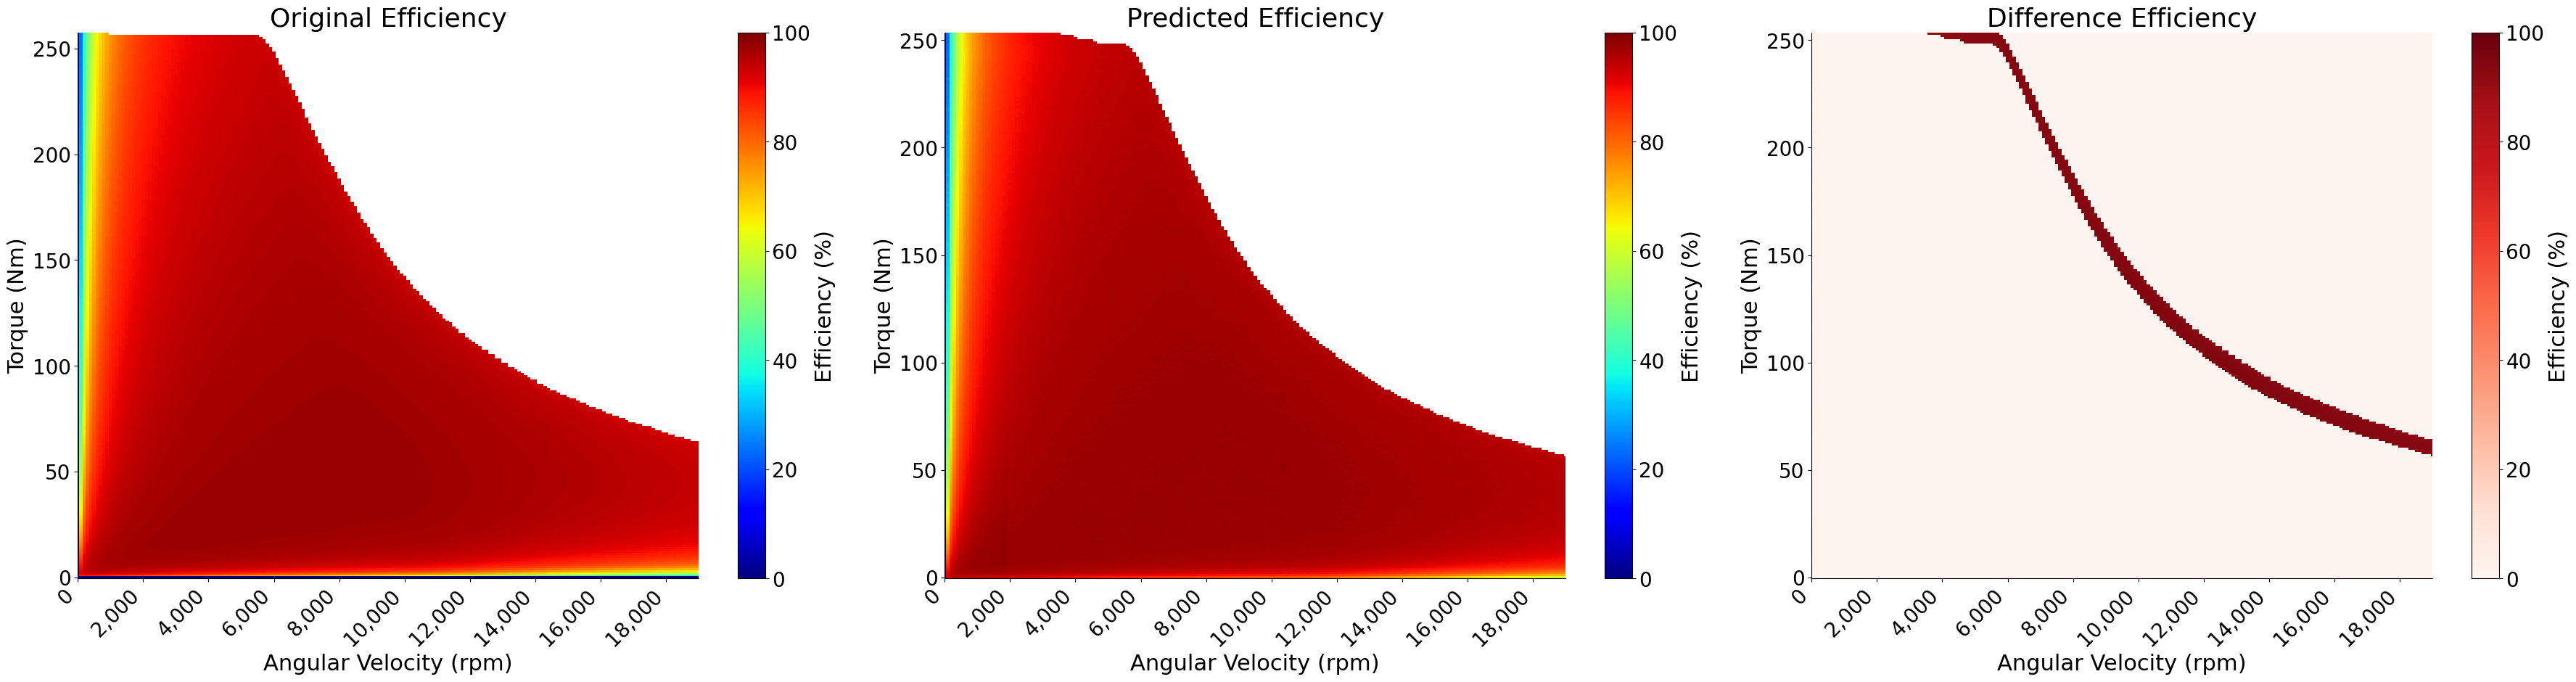
\includegraphics[width=1\textwidth]{./ReportImages/evalkpi3dprediction1.png} 
        \caption{1st Difference Sample} 
        \label{fig:1st Difference Sample}
    \end{subfigure}\hfill
    \begin{subfigure}{1\textwidth}
        \centering
        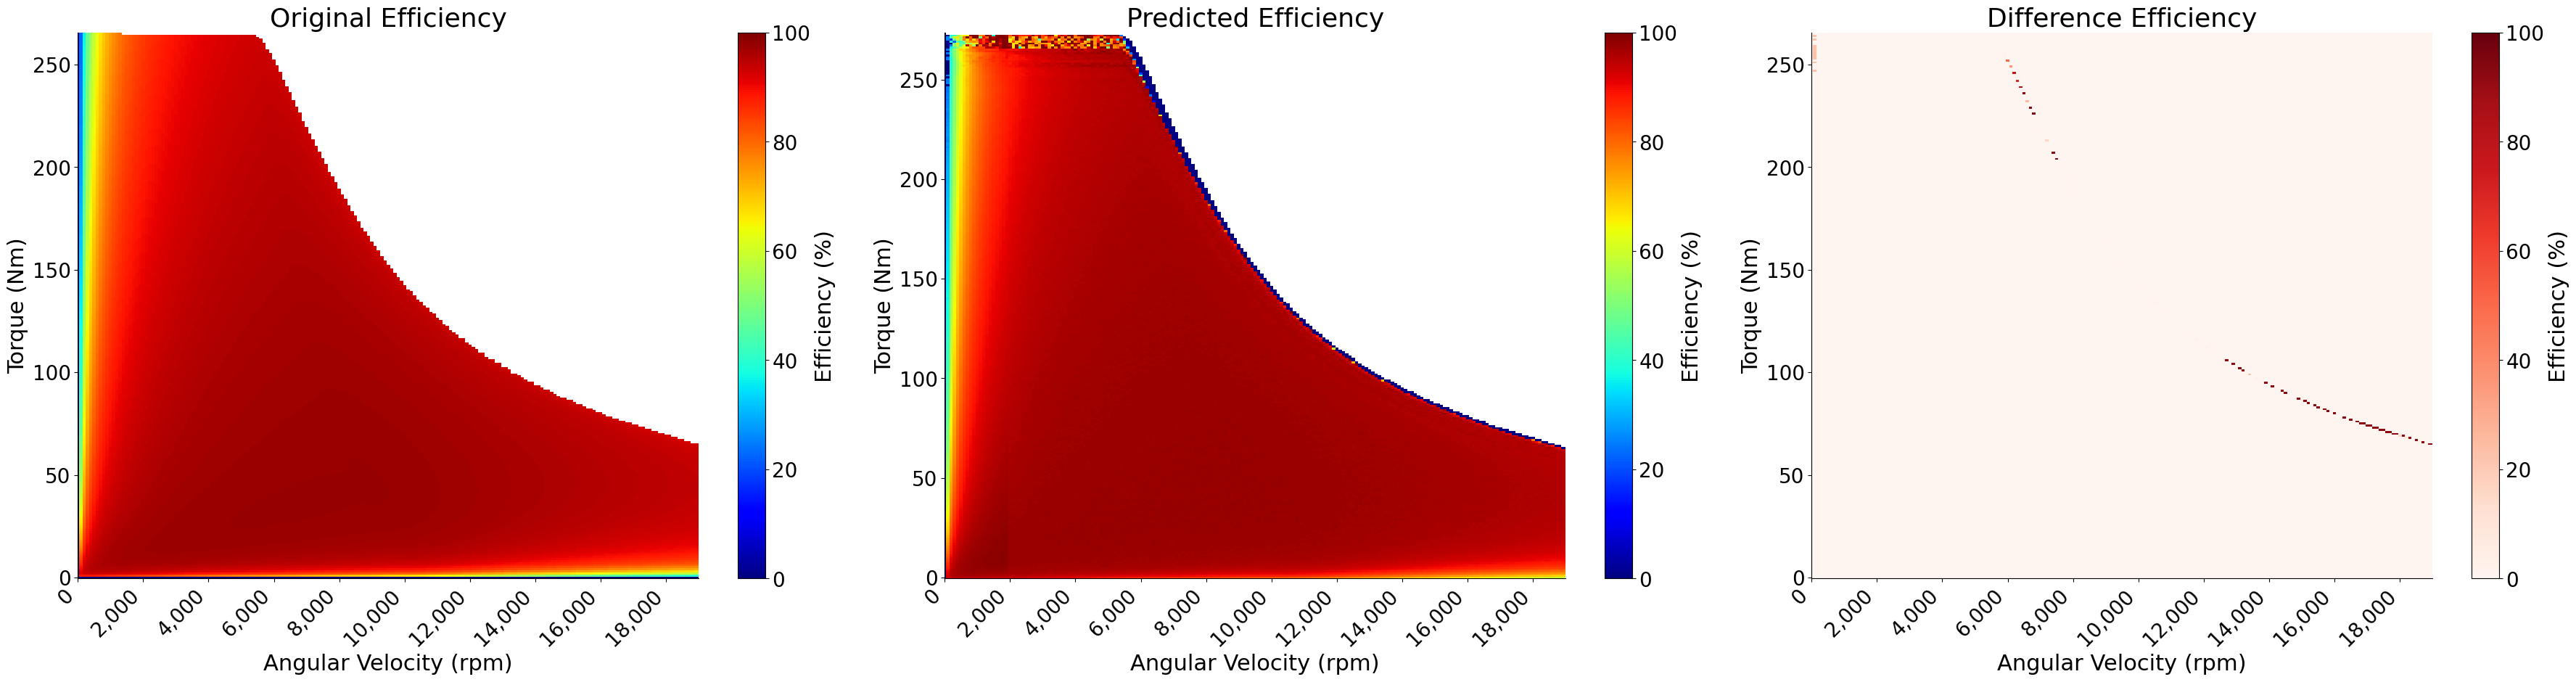
\includegraphics[width=1\textwidth]{./ReportImages/evalkpi3dprediction2.png} 
        \caption{2nd Difference Sample} 
        \label{fig:2nd Difference Sample}
    \end{subfigure}\hfill
    \begin{subfigure}{1\textwidth}
        \centering
        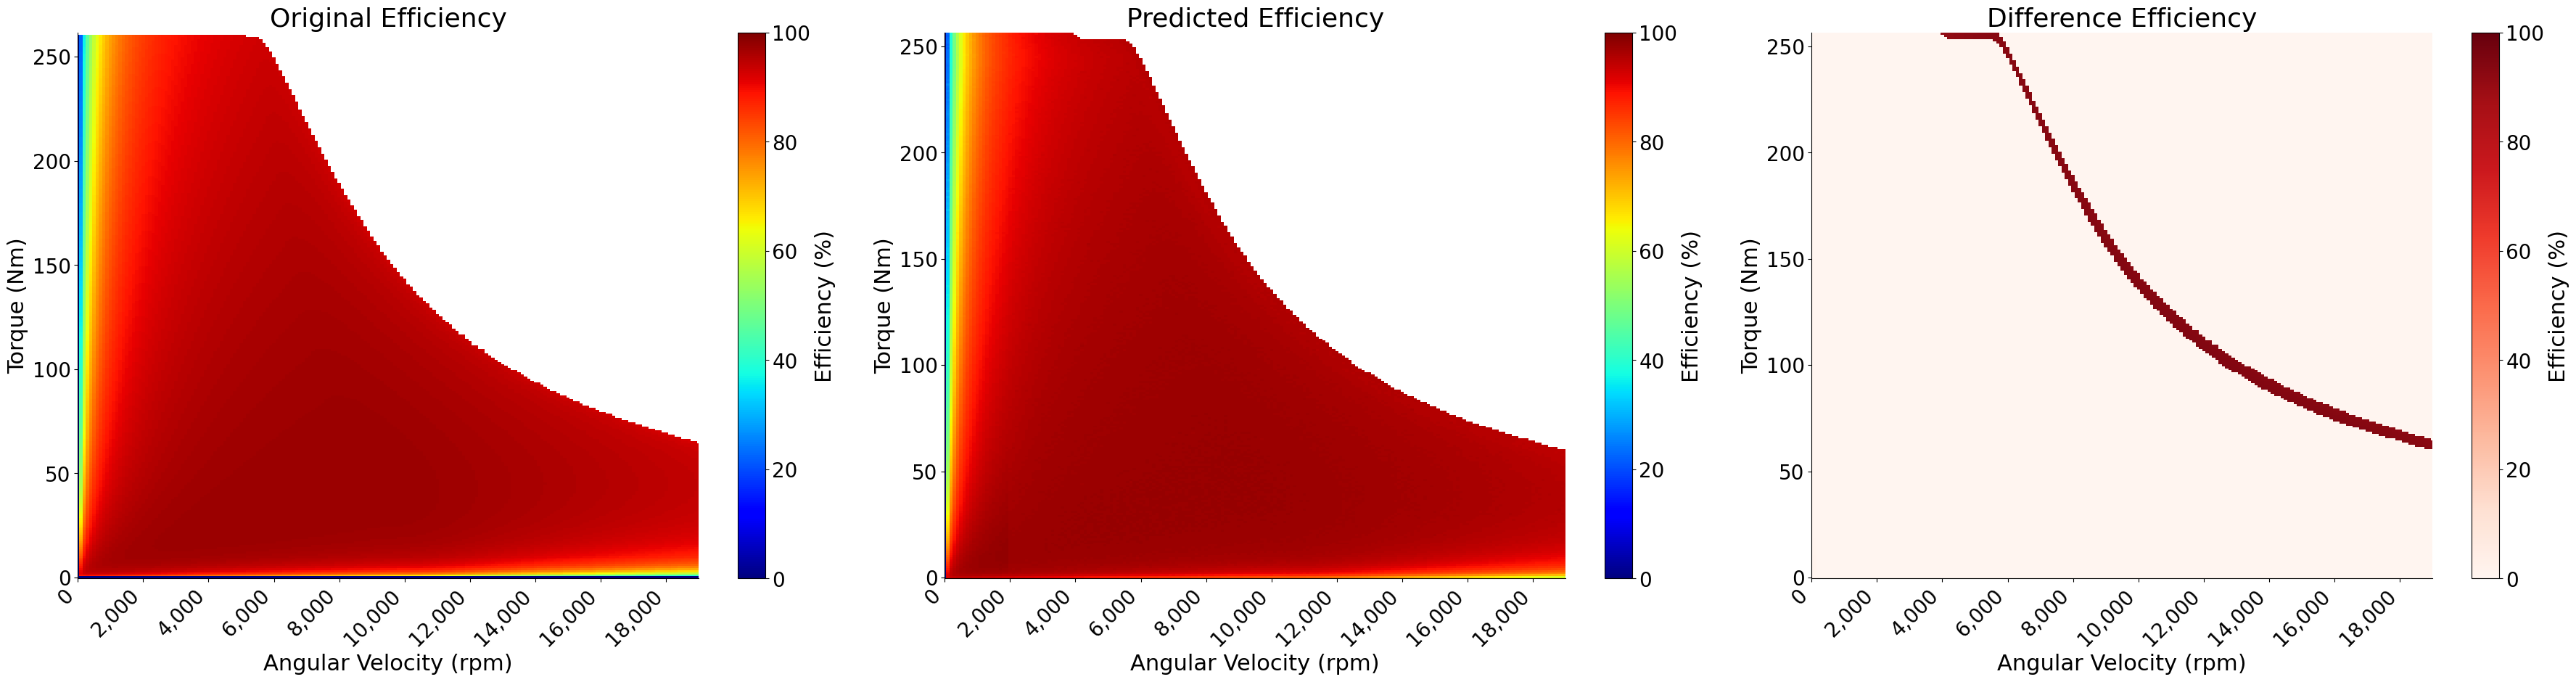
\includegraphics[width=1\textwidth]{./ReportImages/evalkpi3dprediction3.png} 
        \caption{3rd Difference Sample} 
        \label{fig:3rd Difference Sample}
    \end{subfigure}
    \caption{Efficiency \ac{KPI} Predictions Vs Targets Vs Difference with \ac{MLP}},
    \label{fig:Efficiency KPI Predictions Vs Targets Vs Difference with MLP}
\end{figure} 

From a visual perspective, the predictions to relative extent resembles the target and the regularization of the Efficiency \ac{KPI} seems to be already teaching 
the model that the envelope should follow the Torque \ac{KPI} curve shape.  
The curve being sliced off irregularly is the effect of us trying to retain the Torque \ac{KPI} shape as was discussed in Section \ref{sec:Post Processing}.
This could be having negative impacts for the Efficiency \ac{KPI}  when the predictions for the Torque \ac{KPI} are not perfect.
This is yet again a decision to be made based on which of the 2 targets to prioritize. 

We visualize the images for the same samples in Figure \ref{fig:Efficiency KPI Predictions Vs Targets Vs Difference with MLP} however in a smaller scale to accommodate 
a 3rd figure denoting difference overlap. Thus, the figures in \ref{fig:Efficiency KPI Predictions Vs Targets with MLP} serve to give a larger view for comparing and 
contrasting the predictions and its targets.

Additionally, we calculate the RMSE and differences of prediction from the target by truncating the predicted and ground truth matrices to be of common shape.
We also replace \ac{NaN} values with 0s in either if it occurs as the Efficiency \ac{KPI}'s were padded with \ac{NaN}'s to be of the same shape but originally 
had no values as was discussed in Section \ref{subsec:Deep Dive into 3D KPI}.

\begin{figure}[H]
    \centering
    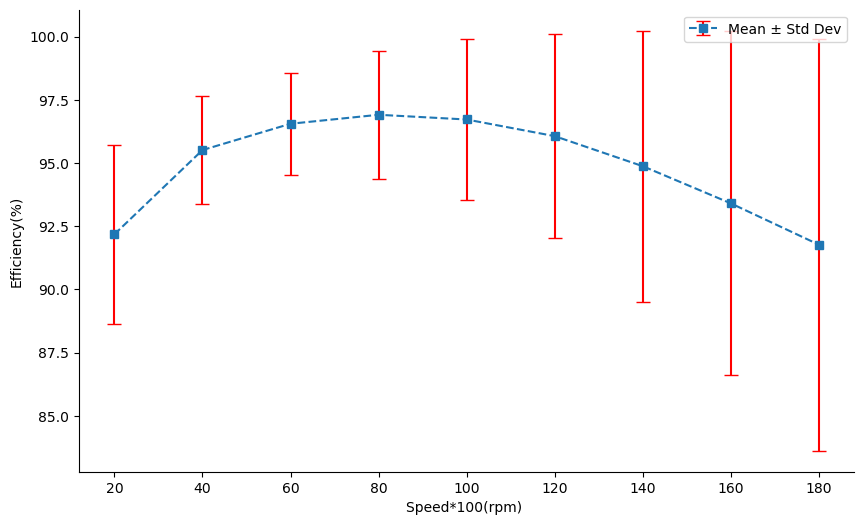
\includegraphics[width=0.8\textwidth]{./ReportImages/stddev_y2_nn_MLP.png} 
    \caption{\ac{MLP} Standard Deviation of Efficiency \ac{KPI} Positive Grid across Angular Velocity Intervals} 
    \label{fig:MLP Standard Deviation of 3D KPI(Efficiency) Positive Grid across Angular Velocity Intervals}
\end{figure}

Figure \ref{fig:MLP Standard Deviation of 3D KPI(Efficiency) Positive Grid across Angular Velocity Intervals} illustrates the standard deviation across different 
angular velocity ranges for the \ac{MLP} predictions as error bar plots.
In comparison to Figure \ref{fig:Standard Deviation of 3D KPI(Efficiency) Positive Grid across Angular Velocity Intervals} we infer that as the speed angular 
velocity increases the target deviations of efficiency values are not so accurately captured by the model.

Efficiency \ac{KPI} is harder to evaluate scoring being a 3\ac{D} plot. There exists 191 angular velocity ranges holding efficiency values.
Since it is infeasible the deviations of the efficiency with respect to all angular velocity intervals, we visualize the Efficiency prediction deviation 
with its respective targets only for specific angular velocities across the entire torque range in Figure \ref{fig:Eval MLP Efficiency RMSE KPI}. Therefore, the 
whole figure encompasses6 subplots for specific angular velocities.
The figure shows the mean Efficiency values and the \ac{RMSE} surrounding it for few samples from the test dataset.
The angular velocities are chosen at equal intervals of 2000 rpm. The Efficiency values are usual range from 0 to 100\% percentage whereas the torque values are shown 
from 0 to approximately 250 Nm which could be the maximum torque value for samples predicted from few random samples of the test dataset.
The \ac{RMSE} of each prediction from its target can be viewed on the twin y-axis.
We can observe that the most deviation occurs towards the higher torque values for each corresponding angular velocity i.e., where the Efficiency envelope starts to taper off.
This anomaly can be explained by the Torque \ac{KPI} predictions not being up to mark as it is responsible for trimming the edges of the envelope.
However it is not only the border of the envelope a question of concern here but also for neighboring values of the envelope specifically from 1/4th the 
angular velocity onwards ie., close to 6000 rpm. 
We donot have any way to teach the model this part of the grid with loss regularization because we cannot estimate the envelope dimensionality having already padded 
the targets to be of the maximum shape referred in Section \ref{subsec:Deep Dive into 3D KPI}. The reason why it deteriorates from 1/4th the angular velocity onwards is 
because the Efficiency \ac{KPI}s envelope starts to converge from around 6000 rpm as we can see in Figure \ref{fig:Efficiency Grid}.
Nevertheless, we see on average among the angular velocities, the \ac{RMSE} is close to 5 which is 5\% deviation from the target values as per Table \ref{tab:Scoring Criteria}.

With the additional loss regularization of constraining efficiency values to be with 100\% as per Equation \ref{eq:Y2 Maximum Efficiency Regularization}, we can now emphasize 
that the efficiency values donot exceed 100. This is evident from the Figures in \ref{fig:Eval MLP Efficiency RMSE KPI} otherwise the mean efficiency would not be constrained 
within each of the subplots, which we force to only display between 0-100\%. Additionally, the figures in \ref{fig:Efficiency KPI Predictions Vs Targets with MLP} and 
\ref{fig:Efficiency KPI Predictions Vs Targets Vs Difference with MLP} would also highlight this anomaly if it occurs since the levels of the contours are also fixed to 
be between 0-100\%. Any values beyond this range would be visualized haphazardly.

To summarize the relatively higher errors are at located in the operating area along the shape of the torque curve.
Observations from the predictions helped to correct few discrepancies in our development for instance in the Efficiency grid we replaced 0s with \ac{NaN} values which 
we later understood were both represented different in the grid. Since Efficiency values can take up values only between 0-100\%, we consider the same as constant 
across plots and use it as a baseline for determining the levels in the contour plot.

\begin{figure}[H]
    \centering
    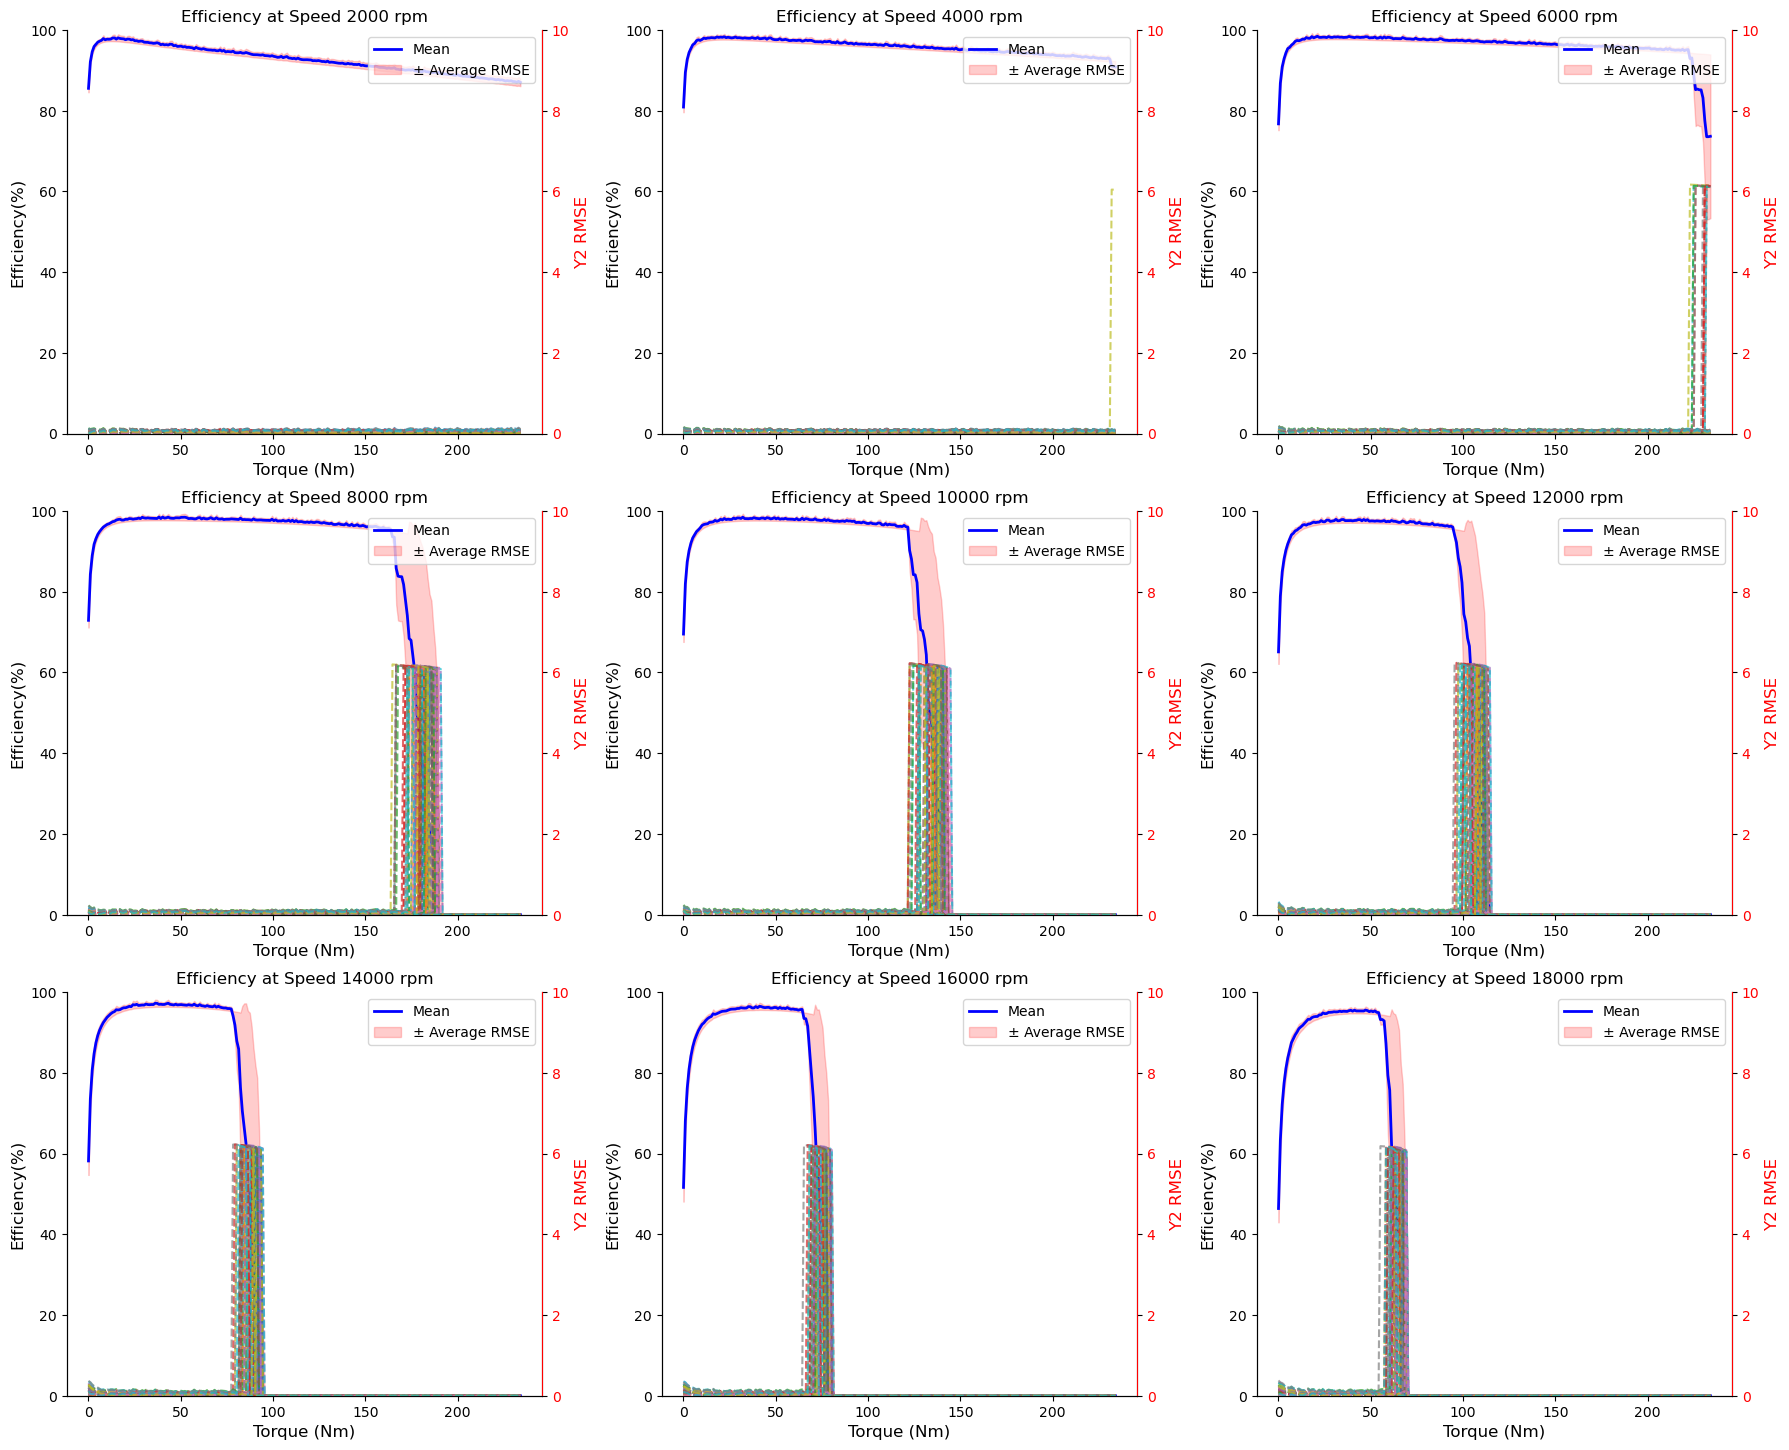
\includegraphics[width=1\textwidth]{./ReportImages/rmse_eta_MLP.png} 
    \caption{Eval MLP Efficiency \ac{RMSE} \ac{KPI}} 
    \label{fig:Eval MLP Efficiency RMSE KPI}
\end{figure}

Figure \ref{fig:Y2 Evaluation Statistics MLP} shows both the Figure \ref{fig:Y2 RMSE} and Figure \ref{fig:Y2 Percentage Difference} from Equations \ref{eq:Y2 Score} 
and \ref{eq:Y2 Percentage Difference} as histogram plots over the entire test dataset with the count of samples on the y-axis.
The histograms for both the figures are the same, nevertheless the intention is to be able to relate to the scores and percentage difference easily die to differing 
value ranges.
\begin{figure}[H]
    \centering
    \begin{subfigure}{0.5\textwidth}
        \centering
        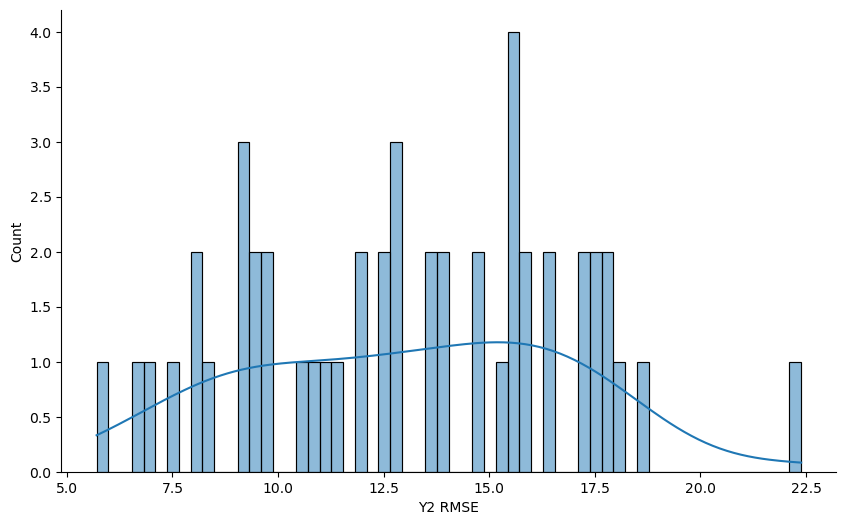
\includegraphics[width=\textwidth]{./ReportImages/score_MLP_y2.png}
        \caption{Y2 \ac{RMSE}}
        \label{fig:Y2 RMSE}
    \end{subfigure}\hfill
    \begin{subfigure}{0.5\textwidth}
        \centering
        \includegraphics[width=\textwidth]{./ReportImages/percentage_diff_MLP_y2.png}
        \caption{Y2 Percentage Difference}
        \label{fig:Y2 Percentage Difference}
    \end{subfigure}
    \caption{Y2 Evaluation Statistics of \ac{MLP}}
    \label{fig:Y2 Evaluation Statistics MLP}
\end{figure}

On an average the \ac{RMSE} is close to 13, which is 13\% deviation from the target values as per Table \ref{tab:Scoring Criteria}.

\begin{figure}[H]
    \centering
    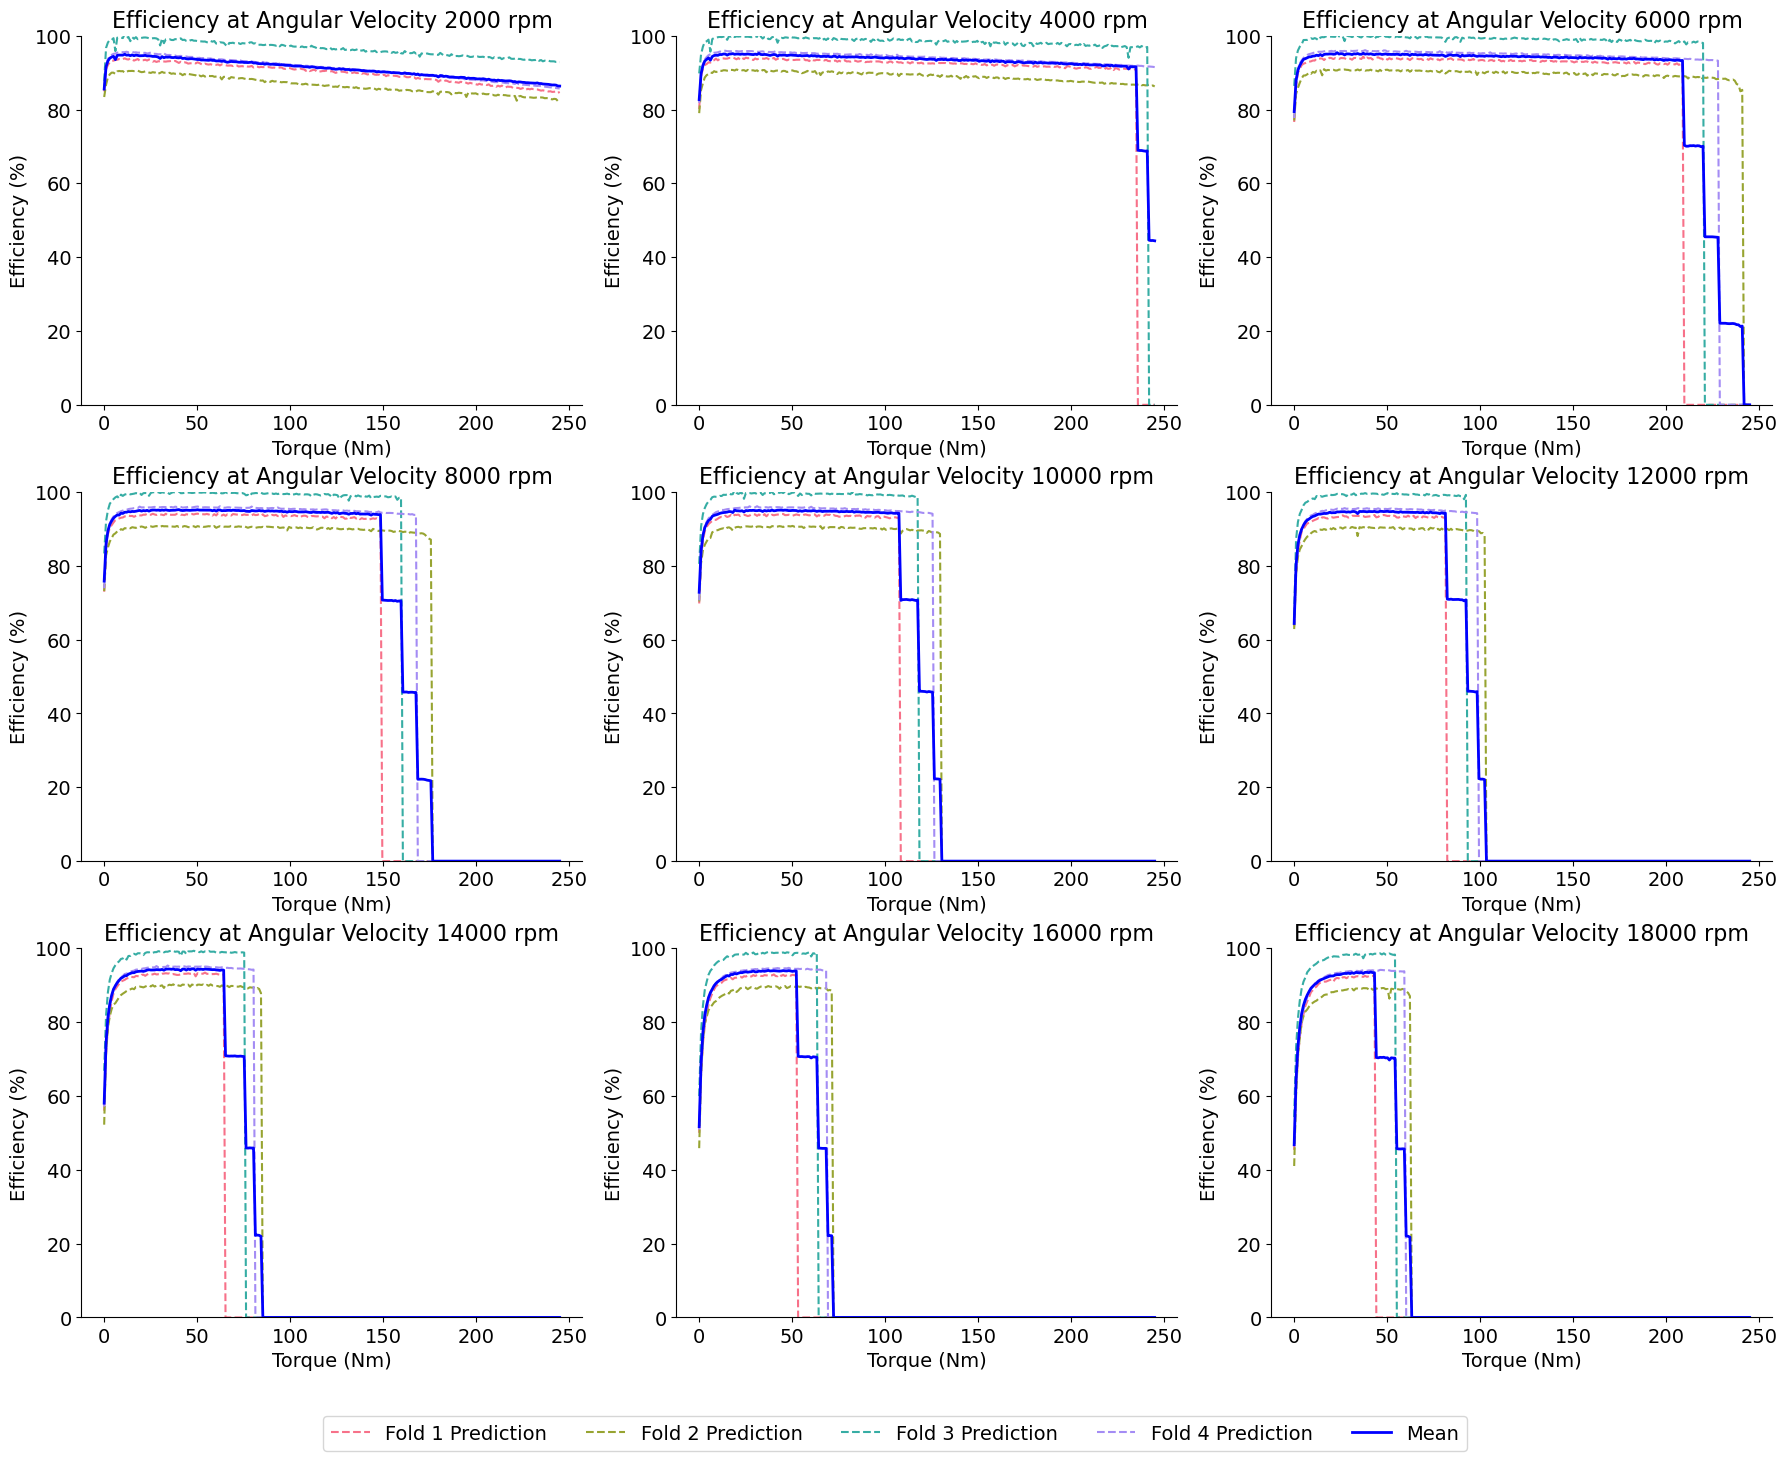
\includegraphics[width=1\textwidth]{./ReportImages/folds_dev_y2.png} 
    \caption{MLP Training Deviation across Folds for Efficiency \ac{KPI}} 
    \label{fig:MLP Training Deviation across Folds for Efficiency KPI}
\end{figure}

Figure \ref{fig:MLP Training Deviation across Folds for Efficiency KPI} illustrates how each fold's prediction of efficiency deviates with the mean of the predictions 
of all folds against different angular velocities. Once again, to overcome the limitation of not being able to evaluate for all angular velocities, the Figure hosts only 6 
subplots for specific angular velocities. From visual inspection we can say the predictions are close enough to the mean of all the Folds predictions.
This figure is a good indicator of the model's generalization performance and needless to mention we have used only 1 sample here for inference from the test dataset.

\section{Results with Baseline}\label{sec:Results with Baseline}

From our observations on how the predictions closely resembled that of the target values in Section \ref{subsec:Deep Dive into 2D KPI} and 
\ref{subsec:Deep Dive into 3D KPI}, we have developed a Baseline model which is intrinsically the average of all samples of the train dataset.

\subsection{Torque \ac{KPI} Results with Baseline}\label{sec:3D Efficiency Grid Results with Baseline}

The Y1 Baseline score for the Efficiency \ac{KPI} is formulated in Equation \ref{eq:Y1 Baseline Score} :

\begin{equation}
    \text{Y1 Baseline Score} = \frac{1}{n} \sum_{i=1}^{n} \underbrace{ \sqrt{\frac{1}{h} \sum_{j=1}^{h} (\bar{y} - y_{ij})^2}}_{Y1\ Baseline\ RMSE}
    \label{eq:Y1 Baseline Score}
\end{equation}
where, \(\bar{y}\) is the Baseline Average mean, \(h\) is the columns of 1D vector, \(Y1\ Baseline\ \ac{RMSE}\) is the \ac{RMSE} for each test sample.

Figure \ref{fig:Baseline RMSE Evaluation for 2D KPI(Torque)} shows the Average \ac{RMSE} and element wise \ac{RMSE} for the test dataset performance with the 
Baseline Model. The figure is similar in structure as the Figure \ref{fig:MLP RMSE Evaluation for 2D KPI(Torque)}, the distinction is in the values being displayed. 
herein, we show the mean of the predictions from Baseline Model and \ac{RMSE} surrounding it for few samples from the test dataset. Additionally, in the twin y-axis, 
the \ac{RMSE} of the Baseline predictions from its target is displayed in dotted lines.

\begin{figure}[H]
    \centering
    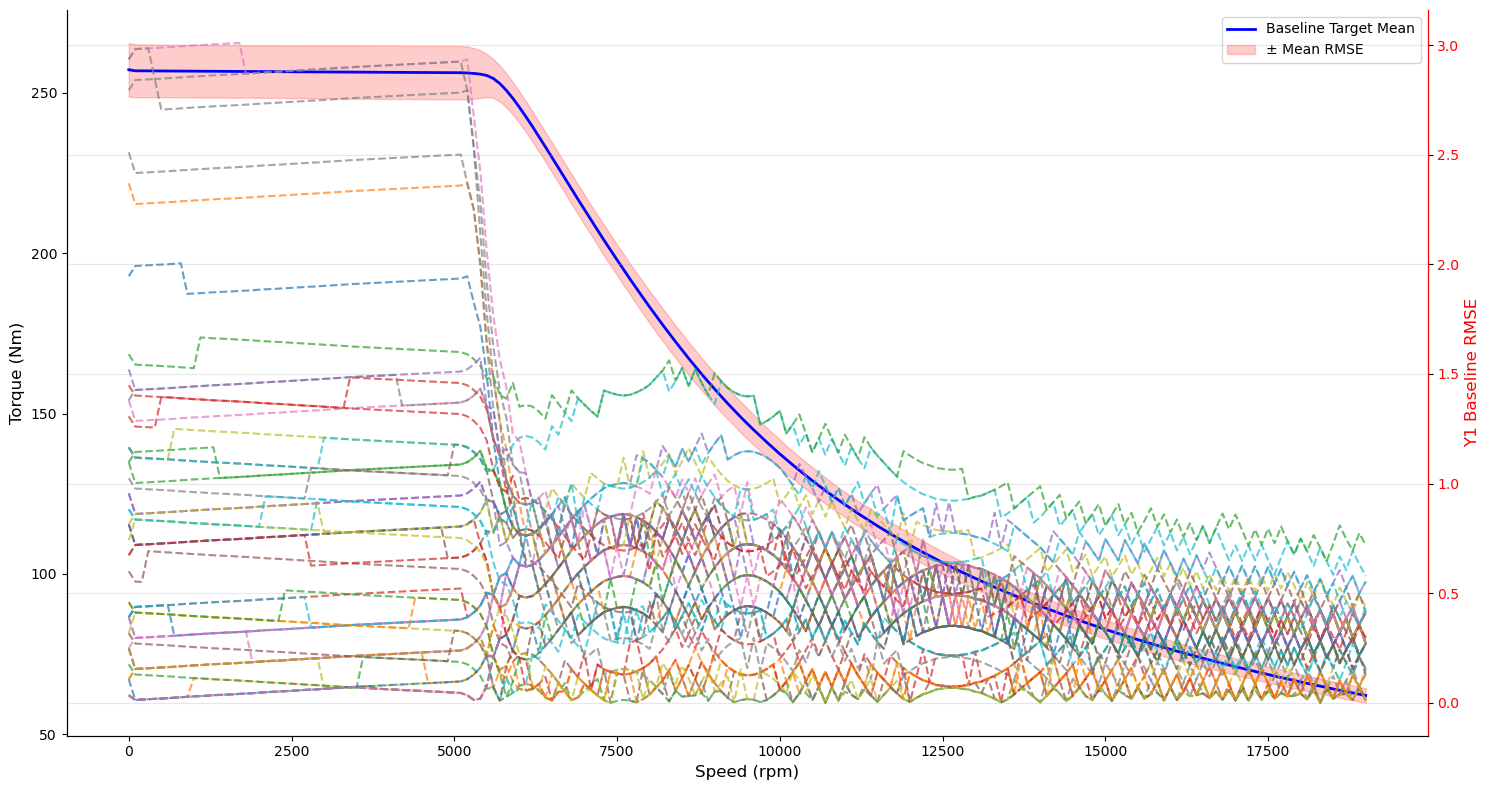
\includegraphics[width=0.75\textwidth]{./ReportImages/RMSE_Baseline_y1.png} 
    \caption{Baseline \ac{RMSE} Evaluation for 2D KPI(Torque)} 
    \label{fig:Baseline RMSE Evaluation for 2D KPI(Torque)}
\end{figure}

We can see that the deviations are at its most towards the beginning of the curve which steadily decreases along the curve. We also observe that there are no 
fluctuations in the curve as compared to the Predictions from \ac{MLP} model in Figure \ref{fig:MLP RMSE Evaluation for 2D KPI(Torque)}.

\subsection{Efficiency \ac{KPI} Results with Baseline}\label{sec:3D Efficiency Grid Results with Baseline}

The Y2 Baseline score for the Efficiency \ac{KPI} is formulated in Equation \ref{eq:Y2 Baseline Score} :
\begin{equation}
    \text{Y2 Baseline Score} = \frac{1}{n} \sum_{i=1}^{n} \underbrace{ \sqrt{\frac{1}{w} \frac{1}{h} \sum_{j=1}^{w} \sum_{k=1}^{h} (\bar{y} - y_{ijk})^2}}_{Y2\ Baseline\ RMSE}
    \label{eq:Y2 Baseline Score}
\end{equation}
where, \(w\) is the rows of 2\ac{D} vector, \(h\) is the columns of 2\ac{D} vector and \(Y2\ Baseline\ \ac{RMSE}\) is the \ac{RMSE} for each test sample.

Figure \ref{fig:Eval Baseline Efficiency RMSE KPI} gives a neat visualization of the Baseline Efficiency \ac{RMSE} with its respective targets for certain angular velocities  
across the entire torque range. This figure is yet again similar in structure to the Figure \ref{fig:Eval MLP Efficiency RMSE KPI} however the efficiency values 
shown now are the predictions of the Baseline model. We infer from the plots that the targets have essentially the same efficiency values across the entire grid.
We arrive at this conclusion from the fact that the only region where we see significant deviation is at the Efficiency \ac{KPI} envelope and we attribute this 
pattern to stem from the corresponding Torque \ac{KPI}'s curve. Thus, the efficiency values are almost the same for more than 3/4th of the grid across all samples.
\begin{figure}[H]
    \centering
    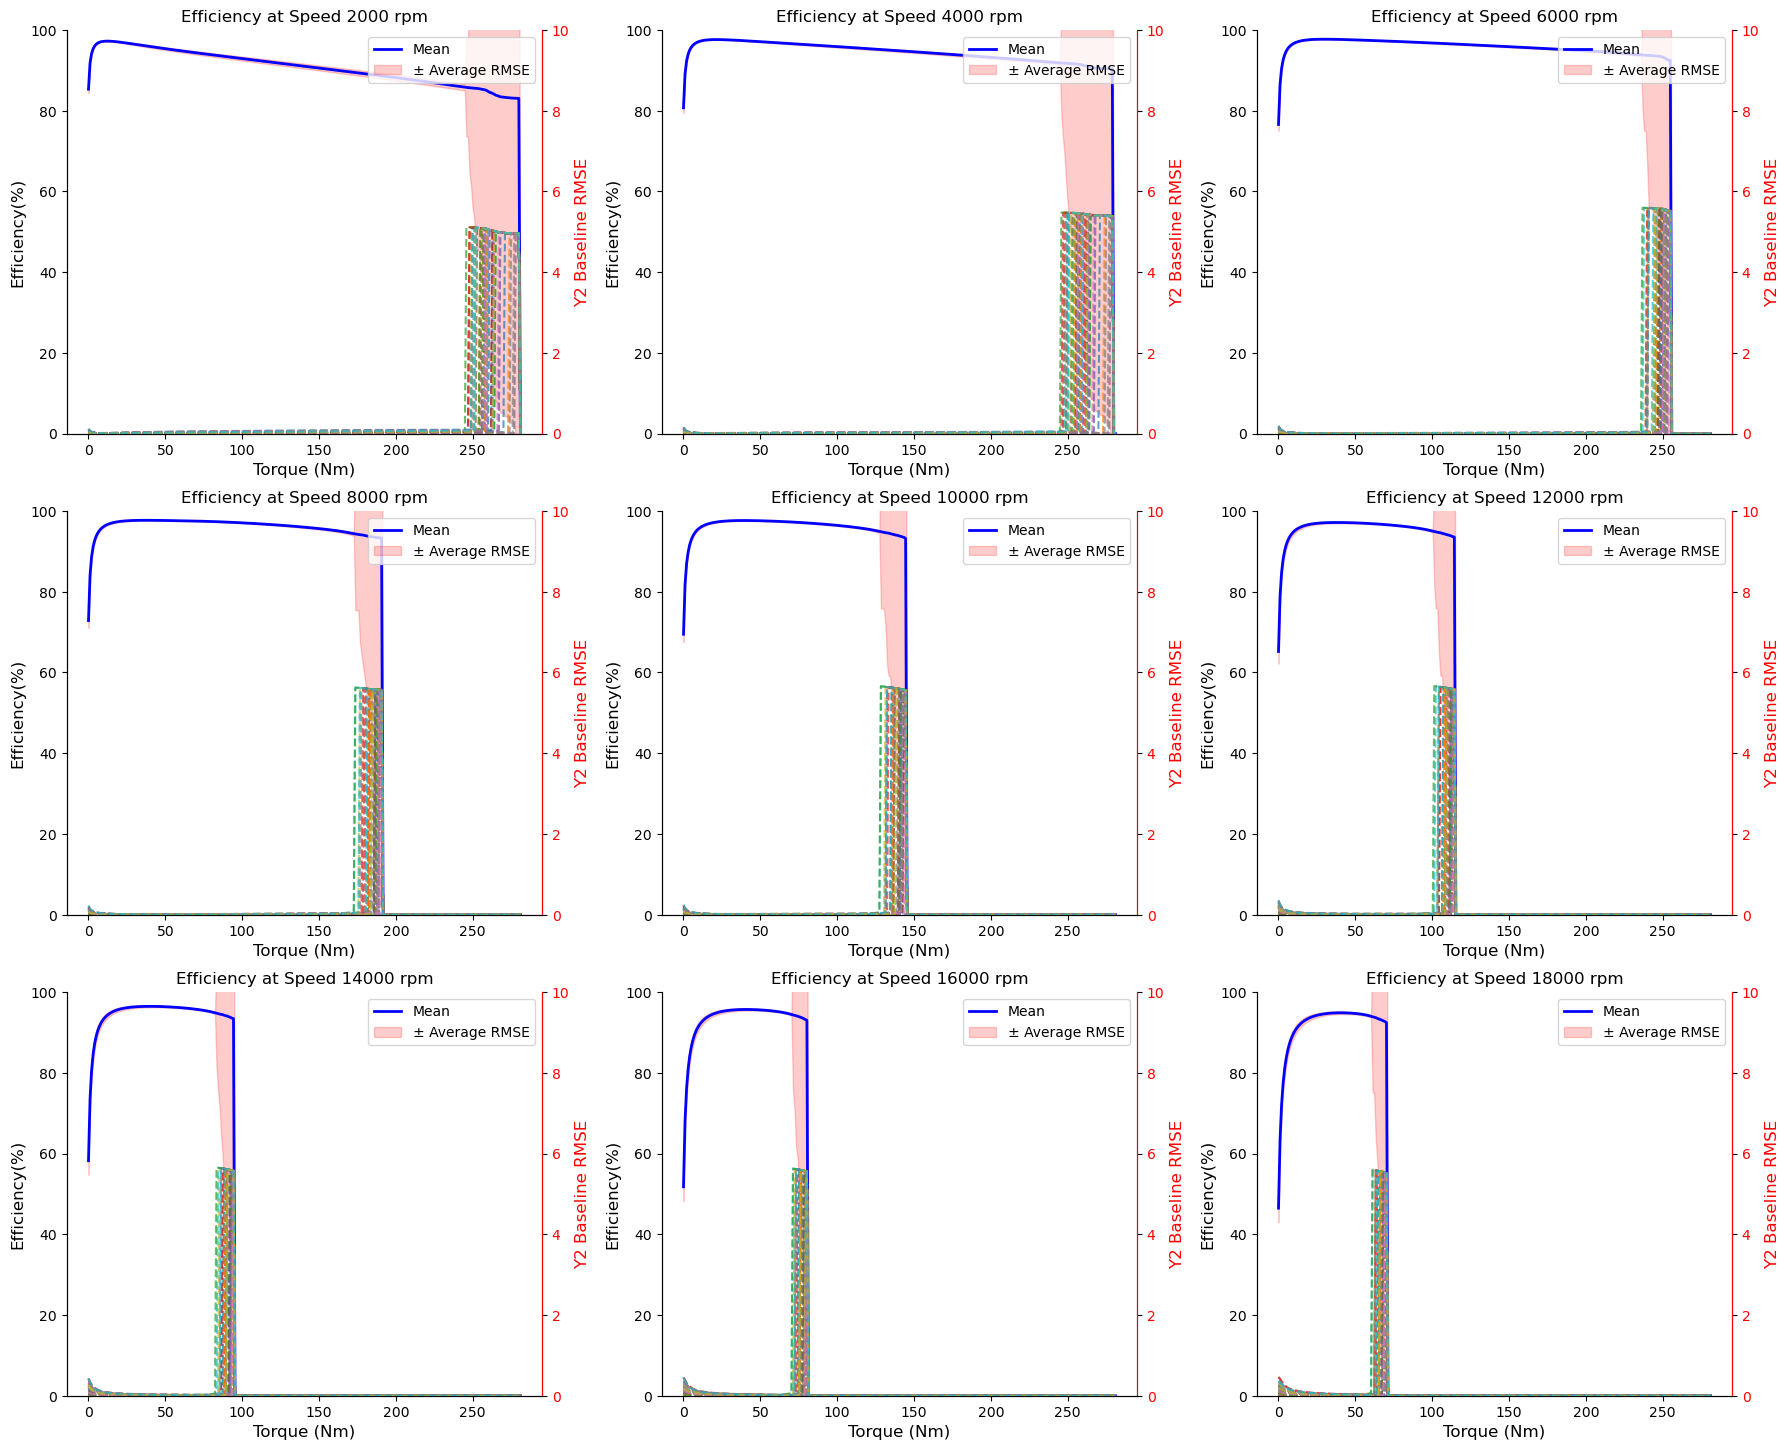
\includegraphics[width=1\textwidth]{./ReportImages/rmse_eta_Baseline.png} 
    \caption{Eval Baseline Efficiency \ac{RMSE} \ac{KPI}} 
    \label{fig:Eval Baseline Efficiency RMSE KPI}
\end{figure}

\section{Results with Smoothening Loss Regularization}\label{sec:Results with Smoothening Loss Regularization}

\subsection{Torque \ac{KPI} Results with Smoothening Loss Regularization}\label{subsec:2D Torque Results with Smoothening Loss Regularization}

Figure \ref{fig:Smoothening Torque RMSE Evaluation for 2D KPI(Torque)} shows the Average \ac{RMSE} and element wise \ac{RMSE} for the test dataset performance 
with the MLP Model with Smoothening Curve regularization discussed in Equation \ref{eq:Y1 Smoothening Loss Regularization}.
We can see that the deviations are at its peak towards the beginning of the curve. 
We also observe that there are fluctuations in the curve but relatively less when compared to Figure \ref{fig:MLP RMSE Evaluation for 2D KPI(Torque)}.
\begin{figure}[H]
    \centering
    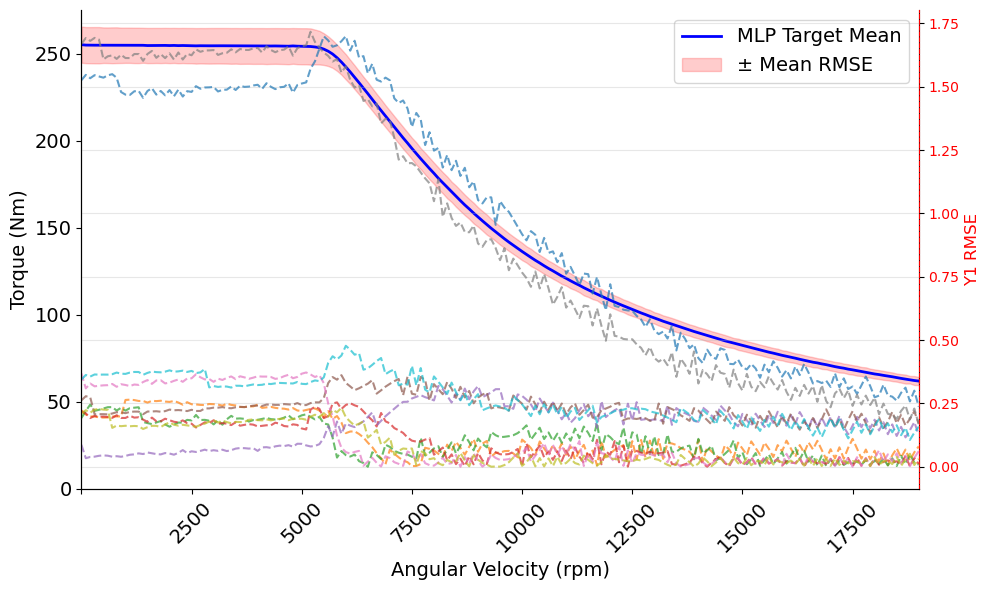
\includegraphics[width=0.75\textwidth]{./ReportImages/RMSE_MLP_Smoothening_y1.png} 
    \caption{Smoothening Torque \ac{RMSE} Evaluation for 2D KPI(Torque)} 
    \label{fig:Smoothening Torque RMSE Evaluation for 2D KPI(Torque)}
\end{figure}

\section{Results with No Loss Regularization}\label{sec:Results with No Loss Regularization}
\subsection{Torque \ac{KPI} Results with No Loss Regularization}\label{subsec:2D Torque Results with No Loss Regularization}

Figure \ref{fig:No Loss Regularization RMSE Evaluation for 2D KPI(Torque)} shows the Average \ac{RMSE} and element wise \ac{RMSE} for the test dataset 
performance with the MLP Model without any regularizations.

\begin{figure}[H]
    \centering
    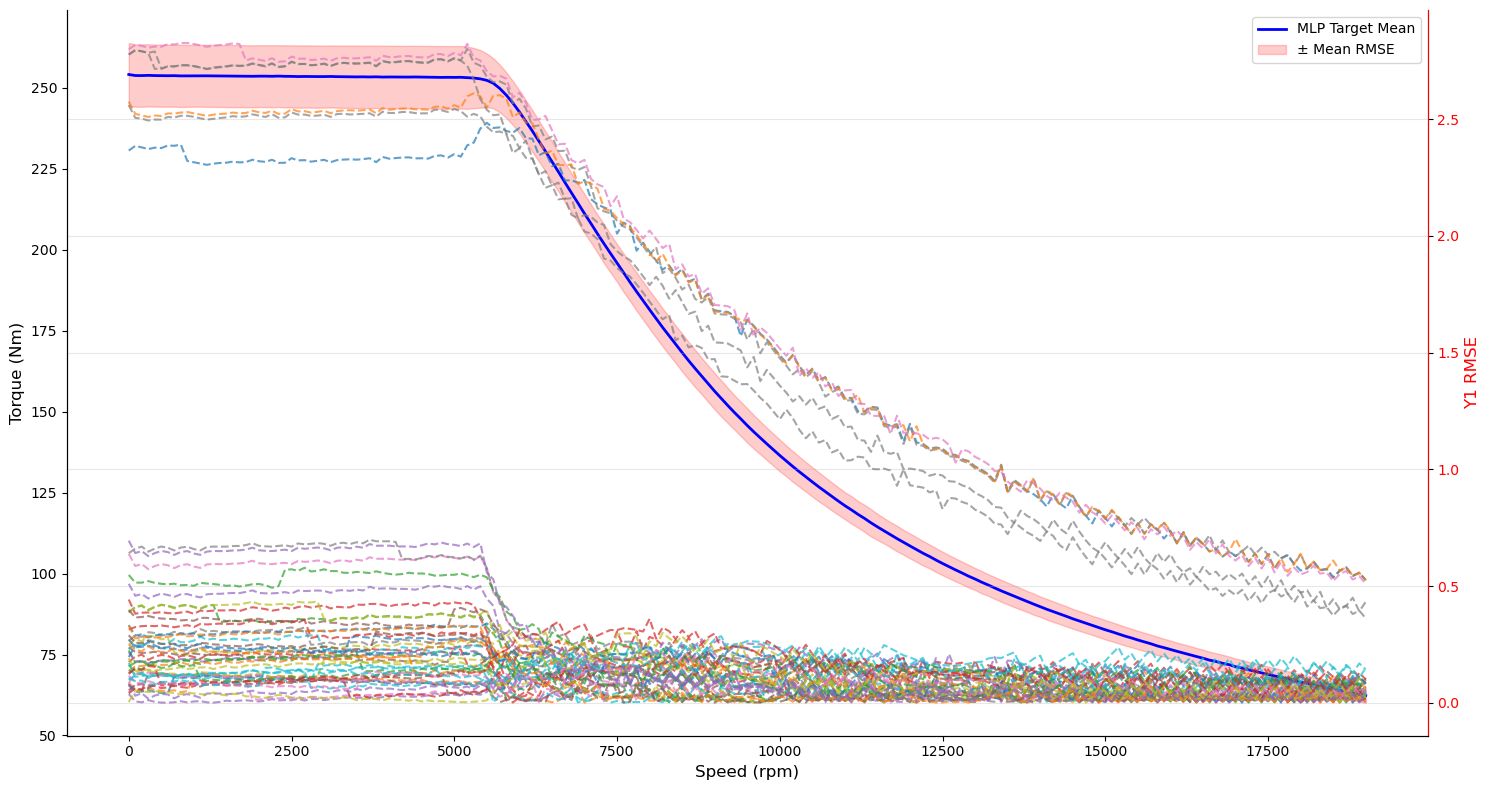
\includegraphics[width=0.75\textwidth]{./ReportImages/RMSE_MLP_no_lossreg_y1.png} 
    \caption{No Loss Regularization \ac{RMSE} Evaluation for 2D KPI(Torque)} 
    \label{fig:No Loss Regularization RMSE Evaluation for 2D KPI(Torque)}
\end{figure}

We can see that the deviations are at its peak towards the beginning of the curve however the \ac{RMSE} for most samples is close to negligible.
We also note there are fewer fluctuations in the curve as compared to the Predictions with Loss Regularizations.
This conclusion prompts us to omit the loss regularization for the Torque \ac{KPI}.

\subsection{Efficiency \ac{KPI} Results with No Loss Regularization}\label{subsec:3D Efficiency Results with No Loss Regularization}

Figure \ref{fig:Eval No Loss Regularization Efficiency RMSE KPI} gives a neat visualization of the Baseline Efficiency \ac{RMSE} with its respective targets 
for specific speeds across the entire torque range. The speeds are chosen at equal intervals of 2000 rpm.
We observe similar patterns to the ones generated with loss regularization in place. This fuels us to also omit the loss regularizations for the Efficiency \ac{KPI}.
\begin{figure}[H]
    \centering
    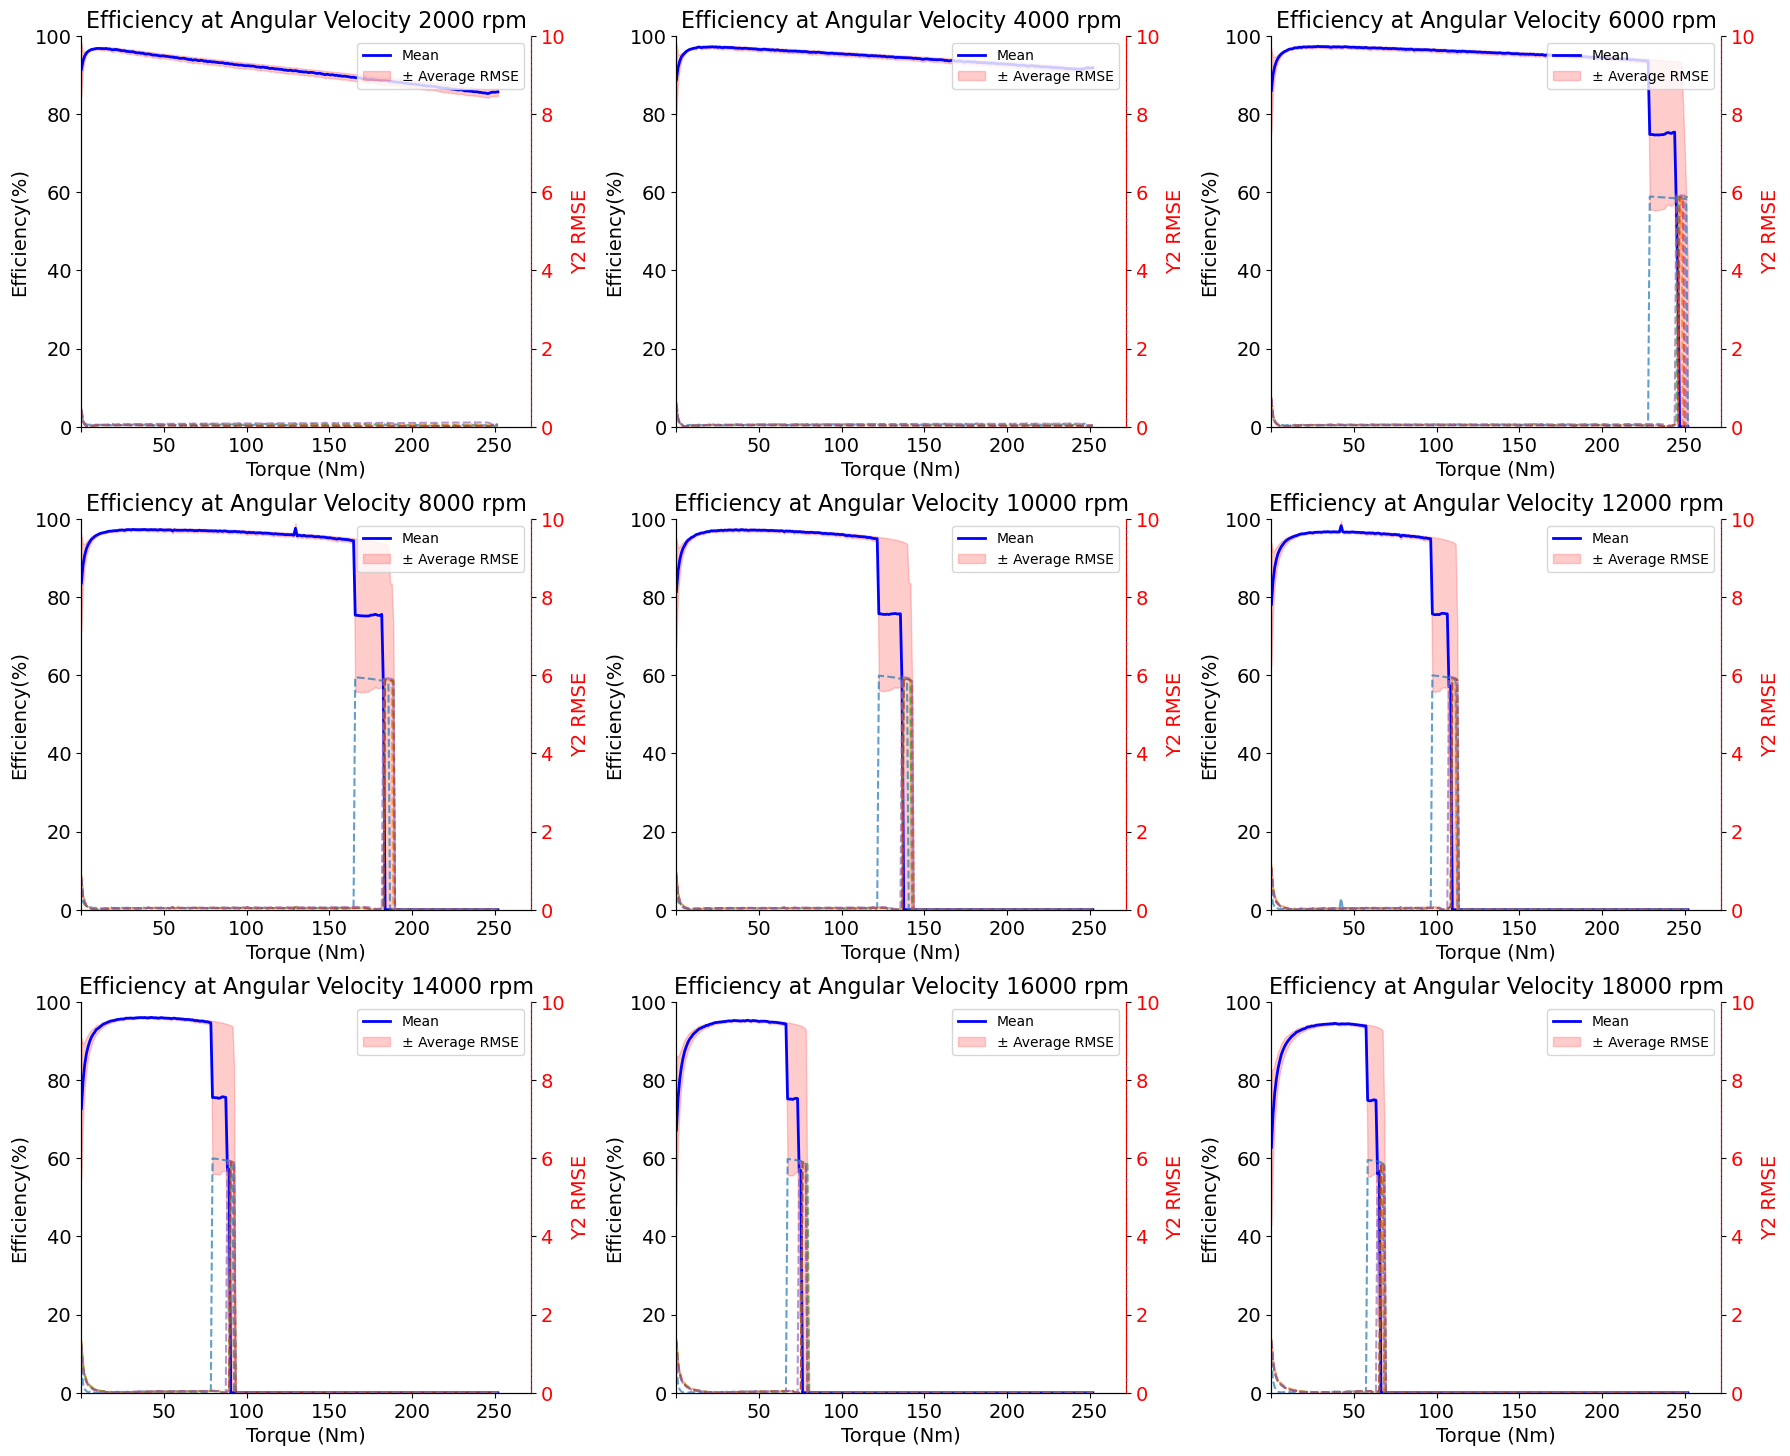
\includegraphics[width=1\textwidth]{./ReportImages/rmse_eta_no_lossreg_MLP.png} 
    \caption{Eval No Loss Regularization Efficiency \ac{RMSE} \ac{KPI}} 
    \label{fig:Eval No Loss Regularization Efficiency RMSE KPI}
\end{figure}

\section{Ablation Studies}\label{sec:Ablation Studies}

We conduct comprehensive ablation studies on the \ac{MLP} model with different loss regularizations and the Baseline model for both our targets.

\begin{minipage}[t]{\textwidth}
    \begin{table}[H]
        \centering
        \begin{tabular}{|p{0.275\textwidth}|p{0.275\textwidth}|p{0.275\textwidth}|}
        \hline {\bf Model} & {\bf Y1 Score} & {\bf Y2 Score}\\
        \hline 
        Baseline & 4.8201 & 15.3708 \\
        MLP\footnote{MLP With Decreasing Y1 Loss Regularization} & 5.1213 & 14.099 \\
        MLP\footnote{MLP With Smoothening Y1 Loss Regularization} & 5.5052 & 15.0257 \\
        MLP\footnote{MLP without both Y1 and Y2 Loss Regularization} & 4.9887 & 12.6612  \\
        \hline
        \end{tabular}
        \caption{Ablation Studies}
        \label{tab:Ablation Studies}
    \end{table}
\end{minipage}

\vspace{1em} % Adjust the space here, e.g., 1em or 2em

Results in Table \ref{tab:Ablation Studies} indicate that our \ac{MLP} model without loss regularizations performance is in par with the Baseline model on the Torque 
\ac{KPI} and has outperformed it on the Efficiency \ac{KPI}. This could be because the regularizations are restrictive and discourage the model to learn better.
The enriched ablation studies we undertook demonstrate the robustness of our method across varying hyperparameter settings.
The inferences shown are strictly speaking from the Double V Magnet Topology which assumed the bulk of the data we had received.

We also show a glimpse of the time conserved with surrogate modelling and relate both approaches how we have demonstrated in the flowchart in Figure 
\ref{fig:EM Design Flowchart}.

\begin{minipage}[t]{\textwidth}
    \begin{table}[H]
        \centering
        \begin{tabular}{|p{0.275\textwidth}|p{0.275\textwidth}|p{0.275\textwidth}|}
        \hline {\bf Approach} & {\bf Time taken(minutes)} & {\bf Hardware}\\
        \hline 
        Surrogate Modelling (Proposed Approach) & 2 mins & 1500 CPU Cores\\
        \ac{FEA} simulations (Current Approach)\footnote{Source : Valeo} & 5 minutes & 32 CPU Cores \& 1 GPU\\
        \hline
        \end{tabular}
        \caption{Compute Time Comparision}
        \label{tab:Compute Time Comparisions}
    \end{table}
\end{minipage}

\vspace{1em} % Adjust the space here, e.g., 1em or 2em

Considering the limitations in dataset, conducting thorough examinations of a substantial volume is typically unfeasible. 
Therefore, the primary purpose of the thesis is to study the possibility of modelling the \ac{KPI}s predictions and our learnings from it.

We also bring to attention that the time of taking 5 minutes to generate \ac{KPI}s per design using the Current Approach highlighted in Figure 
\ref{fig:EM Design Flowchart} is only possible by running the simulator across High Performance Computing machines of nearly 1500 CPU cores in parallel. 
As the number of cores decrease the simulation would take minutes to hours to converge. Additionally, it is the \ac{FEA} simulator in the block that is the culprit of 
consuming time. Another pointer to note is in reality the time needed to generate \ac{KPI}s with Surrogate Modelling is in the range of milliseconds. 
However most time is utilized during the dataset creation in Data Preprocessing phase as reading the excel files take up a significant chunk of the time.
The computing time of the ANN surrogate models varied between 50.3 to 68 ms/case, which makes the surrogates 2,911 to 2,154 times faster than the FE reference simulation, 
respectively. As opposed to \ac{FEA} simulations, the time required to generate predictions for several motor designs is memory bound 
and computation is not so much of a bottleneck since we can potentially run both training and inference across multiple GPUs in parallel.

We have used Python 3.10.14 for our development and the Pytorch library compatible with Cuda.\\
The model was trained on a NVIDIA Tesla V100 \ac{GPU} with 32 GB Memory and the machine we used had 16 CPUs of the Intel(R) Xeon(R) Silver 4208 CPU @ 2.10GHz 
with allocated disk space of 50 GB for our experiments.
Source code is available at \texttt{\href{https://github.com/Lilly-25/Masters-Thesis}{Github Repository}}\footnote{\url{https://github.com/Lilly-25/Masters-Thesis}}.
% the \href{https://github.com/Lilly-25/Masters-Thesis}{GitHub Repository}.

% The experiments were carried out using python 3.7.0, with PyTorch 1.12.1 and PyG 2.2.0. The computer
% used to run the experiments had 8 CPUs of the type High-frequency Intel Xeon E5-2686 v4 (Broadwell)
% processors, with 61GB shared memory, and one GPU of type NVIDIA Tesla V100 with 16GB memory.
% This GPU has 5,120 CUDA Cores and 640 Tensor Cores.

\newpage 

\chapter{Graph Modelling} 

\section{Introduction}\label{sec:Introduction}

Tabular representation of data in itself cannot account for the spatiality of an \ac{EM} design especially on how its different components interact with one another. 
Therefore we presume modelling our usecase as a graph will be more reasonable so that we can exploit graph dynamics and aggregate features that are semantically similar.
A graph can be composed of nodes and edges with their corresponding features in addition to the graph attributes.
The graph attributes contain the information relevant to the graph as a whole whereas the node features captures the information of the node's role in the network and 
likewise the edge features captures the information of the edge's role in the network. Graphs also take into account their respective neighbourhoods.

\ac{GNN}s in general function by making use of \ac{MP} which is a recursive algorithm that aims to learn a representation vector for each node. 
\ac{MP} is based on the graph structure and initial node features. Over each hop of successive neighbourhoods in the graph, the information of 
neighbouring nodes of a node are shared across as messages and aggregated and the initial node is recursively updated with this information. 
This continues until there are no more nodes to traverse within the graph.
Thus, at the end of the \ac{MP} algorithm, each node in the graph would have a good understanding of the other nodes within the same graph.
Therefore, the final representation will be rich enough to have captured all the information within the graph and can be used for downstream tasks.\\

On the basis of the directionality of edges within graphs, they can have the following taxonomy: \cite{GNN-2019}:
\begin{enumerate}
    \item Directed Graph - A graph in which the edges have a direction from source node to its target node.
    \item Undirected Graph - A graph whose Adjacency matrix is symmetrical such that for each edge there will be its respective reverse edge in the opposite direction.
\end{enumerate}

In addition to their ability to incorporate both entity features and network features into a single, simultaneously trained model, most \ac{GNN}s scale linearly with 
the number of edges in the network, making them applicable to large networks. A huge benefit of \ac{GNN}s in practical use cases is that they are inductive rather 
than transductive. While transductive model can only be used on the specific data that was present during training, inductive models can be applied to entirely new 
data without having to be retrained. This is defended by Johannessen et al. in \cite{ML HGNN-2023}
A hallmark of \ac{GNN}s is that they can efficiently learn the architecture parameters from the training data as demonstrated by Owerko et al. in \cite{PO GNN-2018}.

\ac{GNN}s cannot be too deep with layers due to the oversmoothing problem. 
This is because the \ac{MP} algorithm would have already traversed over all hops and made all features indistinguishable from one another.
Besides a deep \ac{GNN} would have a large number of parameters and would be computationally expensive to train.
\cite{GCN-2018} sheds light on the oversmoothing concern faced by Graph Convolutional Networks.
Studies also tells us that it can be mitigated by including residual connections in the network \cite{RHGNN-2022}.\\

Researchers have broadly classified \ac{GNN}s following 2 distinct paradigms:
\begin{enumerate}
    \item \textbf{Homogeneous \ac{GNN}} \\
        Homogeneous \ac{GNN} are designed for graphs with a single type of nodes and edges. 
        \ac{MP} is done for neighbouring nodes and edges over hops until it learns a representation equivalent from its neighbours.
        Homogeneous \ac{GNN} are typically build to capture the structural information within a graph.
        These models are effective when the node and edge heterogeneity is negligible cited by the authors of \cite{EHR HGNN-2024}. 
    \item \textbf{Heterogeneous \ac{GNN}} \\    
        Heterogeneous \ac{GNN} are designed for graphs with differing types of nodes and edges implying difference in features as well as dimensionality.
        The authors of \cite{{HNNC-2023}} argue that each type of node and edge reveal unique semantic information.
        As a single function cannot cater to each type, hence different \ac{MP} and node updating functions needs to be implemented for each edge and node type respectively.
        Therefore \ac{MP} is conditioned on the node and edge type thus allowing the flow of information to be more controlled. 
        In addition to the structural information, Heterogeneous \ac{GNN}s also excel to capture semantic information within the graph.
\end{enumerate}

\subsection{Applications}\label{subsec:Applications}

\ac{GNN} predictions can be categorized broadly into : \cite{GNN-2019}
\begin{enumerate}
    \item Node Level Prediction - represents node classification and regression
    \item Edge Level Prediction - focuses on edge classification and link prediction
    \item Graph Level Prediction - relate to graph prediction tasks.\\
    Incidently our task is a Graph Level prediction.
\end{enumerate}

Some of the well known \ac{GNN} tasks can be seen in Figure \ref{fig:GNN Predictions} :
\begin{enumerate}
    \item Graph Classification - 
    \item Node Classification - 
    \item Link Prediction - 
    \item Community Detection - 
    \item Graph Embedding - 
    \item Graph Generation - 
\end{enumerate}

\begin{figure}[H]
    \centering
    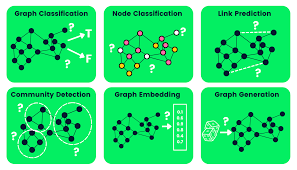
\includegraphics[width=0.5\textwidth]{./ReportImages/GraphTasks.png} 
    \caption{\ac{GNN} Predictions Source :WWW} 
    \label{fig:GNN Predictions}
\end{figure}

\ac{GNN}s have several applications where data are generated from non-Euclidean domains and are represented as graphs with complex relationships 
and interdependency between objects \cite{GNN-2019}. Figure \ref{fig:GNN Applications} illustrates various \ac{GNN}s applications ranging 
from Recommendation Systems, Chemistry, Traffic, Academic Networks, Information Networks to Social Networks \cite{HGNN-2020}.
\begin{figure}[H]
    \centering
    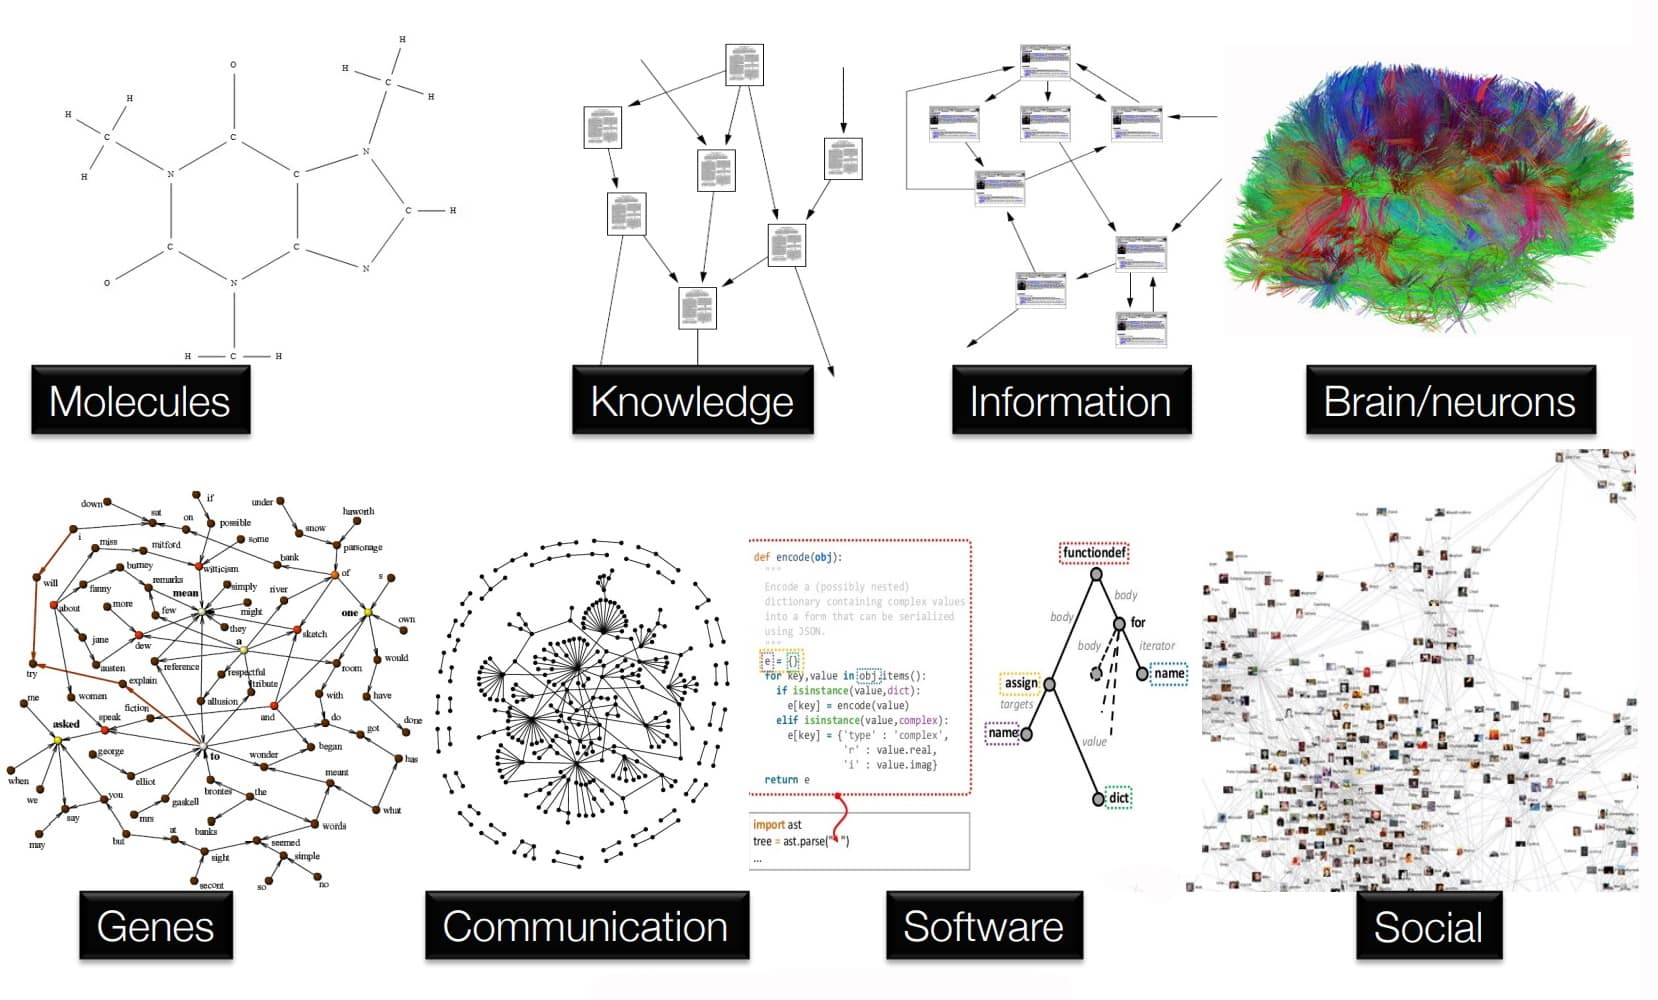
\includegraphics[width=0.95\textwidth]{./ReportImages/GraphApplications.png} 
    \caption{\ac{GNN} Applications Source :WWW}
    \label{fig:GNN Applications}
\end{figure}

These networks are generally represented by a giant graph in which case graph batching, splitting are unique.
However our task requires us to build 1 graph each for each \ac{EM} variant.

\section{Heterogeneous \ac{GNN}}\label{sec:Heterogeneous GNN}

Graphs are ubiquitously heterogeneous because of its capability to have different node and edge types on top of its inherent graph feature to abstract and model 
relations between objects.\\
Heterogeneous \ac{GNN}s also takes into account homophily ie., nodes close on a network have similar embeddings \cite{HGNN-2020} this is in essence the structural 
property and is true for all \ac{GNN}s. We largely adopt the commonly used notations from \cite{ML HGNN-2023} and reformulate it slightly for our task. \\

\textbf{Heterogeneous Networks}

Given a directed graph \( \mathcal{HG} = (V, E, X, R, T_v, T_e, \phi, \psi) \).

The sets of possible node types can be represented as: \( T_v = \{ \phi(v) : \forall v \in V \} \) and the sets of possible edge types 
can be represented as: \( T_e = \{ \psi(e) : \forall e \in E \}.\) 

Each node \( v \in V \) has a node type \( \varphi(v) = \nu \in T_v \), where \( \varphi(\cdot) \) is a node type mapping function. 
Further, for \( \varphi(v) = \nu \), \( v \) has features \( x_v^{\nu} \in X^{\nu} \), 
where \( X^{\nu} = \{ x_v^{\nu} \mid v \in V, \varphi(v) = \nu \} \) and \( X = \{ X^{\nu} \mid \nu \in T_v \} \). 
The dimension and attributes of the node feature \( x_v^{\nu} \) may be different for different node types \( \nu \). 

Further, let us denote by \( e_{uv}^{\varepsilon} \) an edge of type \( \varepsilon \in T_e \) pointing from node \( u \) to \( v \). 
Each edge \( e_{uv}^{\varepsilon} \) has features \( r_{uv}^{\varepsilon} \in R^{\varepsilon} \), 
where \( R^{\varepsilon} = \{ r_{uv}^{\varepsilon} \mid u, v \in V \} \) and \( R = \{ R^{\varepsilon} \mid \varepsilon \in T_e \} \). 
Just like for nodes, the edge features may have different dimensions for different edge types.

When \( |T_v| = |T_e| = 1 \), the graph degenerates into a homogeneous graph \cite{SE HGNN-2023}.

Heterogeneous \ac{GNN}s aim to learn a representation vector \( \mathbf{h}^{(L)}_v \in \mathbb{R}^{d_L} \) for each node \( v \) after \( L \)-layer transformations, 
based on the graph structure and the initial node feature \( \mathbf{h}^{(0)}_v \in \mathbb{R}^{d_0} \) \cite{REF HGNN-2021}.\\

\textbf{Metarelation}

For an edge \( e = (s, t) \) linked from source node \( s \) to target node \( t \), its meta relation is denoted as
\(
\langle \tau(s), \varphi(e), \tau(t) \rangle.
\)
This is in essence the relation triple ie.,  \(  (node type of s, edge type, node type of t) \) used commonly in Knowledge Graphs.\\

\textbf{Metapath}

Given a path
\(
\mathcal{P} = T_{v1} \xrightarrow{T_{e1}} T_{v2} \xrightarrow{T_{e2}} \cdots \xrightarrow{T_{vk}} T_{ek}
\), 
if the path describes the composition of edges by its types \( T_{e1} \circ T_{e2} \circ \cdots \circ T_{el} \) between nodes of type \( T_{v1} \) and \( T_{vl} \) and 
$\circ$ denotes the composition operator then the path is called a metapath. The length of the metapath can be calculated from its magnitude i.e, \textit{l-1}. 
The metapath is also the sequence of many metarelations.  If all the combinations of nodes and edges in the graph are used, then the total number of metapaths would 
increase exponentially with the number of node and edge types. Hence, the reason to subselect only few metapths that are significantly most relevant for the task at hand. 
Metapath selection requires domain knowledge to be able to choose those which are most semantically meaningfull and let the Heterogeneous \ac{GNN} use only these paths 
for learning the graph. \\


\textbf{Metapath-based Neighbors}

Given a node \( v_1 \) and a meta-path \( \epsilon \) in a heterogeneous graph, the neighbors \( N_{v_1}^{\epsilon} \) of 
node \( v_1 \) based on the meta-path \( \epsilon \) are defined as the set of nodes connected to \( v_1 \) via the meta-path \( \epsilon \). 
This set of neighbors based on the meta-path also includes \( v_1 \) itself.\\

Heterogeneous \ac{GNN} generally work by having separate non linear functions convolve over each edge type during message computation and over each node type when aggregating the learned information. \\
The graph structure of \( G \) can be represented by a series of adjacency matrices \(\{A_r : r \in T_e\}\). 
For each relation \(r_{c_t c_s} \in R\), \(A_{c_t c_s} \in \mathbb{R}^{|V_{c_t}| \times |V_{c_s}|}\) is the corresponding 
adjacency matrix where the nonzero values indicate positions of edges \(E_{c_t c_s}\) of the current relation.\\

Metapaths are composite relationships between nodes that help to capture the structural information of heterogeneous graphs.\\

The Metapaths in Heterogeneous \ac{GNN}s are divided into 2 streams:
\begin{enumerate}
    \item Metapath based method\\
    It aggregates the neighbourhood features of the same semantic first and then fuses different semantic information.
    \item Metapath free method\\
    It aggregates message from neighbourhood of the same hop for all node types and so captures both structural and semantic information simultaneously.
\end{enumerate}

Multiple \ac{MP} operations are done across different metapaths which are finally aggregated into a new representation for the node.\cite{ML HGNN-2023}.\\
Each metapath captures the proximity of nodes in a graph from a specific semantic view \cite{HGNN-2020}.

% During runtime, the \ac{MP}-\ac{GNN} algorithm would need to iterate over edge type dictionaries during message computation and over node type dictionaries during node updates.
\section{\ac{GNN} Literature Review}\label{sec:GNN Literature Review}

Existing works for instance Yu et al. in \cite{PR-HGNN-2024} model heterogeneous graphs by splitting the graph into multiple 
homogeneous subgraphs based on their node types each retaining an aspect of the heterogeneity.
This is ineffective in exploiting hidden rich semantic associations between different types of edges for large scale multi-relational graphs.
However Zhu et al. \cite{RSHGNN-2019}'s work does not undertake this methodology and is also independent of metapaths making it effective 
in dealing with large number of complex relations.\\
Bias Amplification is a known problem most prevalent in recommender systems where the model is biased to certain outputs due to the training data statistics.
It can be handled much better when a graph is modelled as a heterogeneous graph as is shown in \cite{EV HGNN-2023} this is because differing 
edge types capture varying types of relationships in the graph. \\
Modelling Heterogeneous Graphs with metapaths generally require domain specific knowledge as metapaths are customized. 
In order to combat this, Hu et al. in \cite{HGT-2022} has used meta relations instead and a unique adjacency matrix for each edge type.\\
Works by Melton et al. in \cite{MHGNN-2023} also use metarelations to extract soft metapaths and does message passing over multi-hop neighborhood of nodes. \\
Metarelations are most often used in knowledge graphs as it contains richer schema. 
Such meta relations are shallow embeddings and not as deep as the meta paths as clarified by Yang et al. in \cite{HGNN-2020}. \\
One such work by Zou et al. in \cite{HNNC-2023} proposes a heterogeneous network node classification model which converts the 
heterogeneous network into multiple semantic graphs through metapaths. The polynomial graph convolutional kernel is also described in this paper.\\ 
Li et al. in \cite{GCN-2018} demystifies the Graph Convolutional Network and addresses the Laplacian oversmoothing concern by self-training or co-training the model.
Although it makes classification problem easier over multiple hops the features among different clusters will be the same.
GCN achieves this by breaking down the heterogeneous graph into multiple homogeneous ones, one for each edge type. 
In each layer, GCN is applied to each homogeneous graph, and the resulting node embeddings are element-wise summed to form the final output. 
In RGCN, during message passing, neighbors under the same edge type will be aggregated and normalized first. 
A drawback of RGCN is that it does not take node heterogeneity into account. \\
Most of the existing works demonstrated by Yang et al. in \cite{HGNN-2020} also do not consider the edge features in their model. 
However Johannessen et al. in \cite{ML HGNN-2023} uses edge features as transactions in a financial network to detect cases of money laundering.
It also breaks down the large heterogeneous graph into subgraphs based on different node type-edge type combinations. 
The paper also brings to light that GraphSAGE does not incorporate the edge weights.\\
However, the \ac{MP} neural network framework applies a learned message-passing function that utilizes edge features.\\
Additionally Chana et al. in \cite{EHR HGNN-2024} has used heterogeneous \ac{GNN}s to model the heterogeneity and sparsity in Electronic 
Health Records of patients. This work takes into account the relational features of the dataset which is arguably the most important factor in this domain. 
Their work also claim to learn its multi-task nature. However we note that this paper uses meta relations but donot factor in edge features.\\
Gilmer et al. in \cite{QC-MP-2017} introduces modelling that makes it capable of learning features of molecular graphs directly and is 
invariant to graph isomorphism. Graph isomorphism is the property of graph being similar even when the ordering of nodes and edges are different.
They also suggest that edge features in the network can be learned by introducing hidden states for all edges in the graph and updating them.
It also implements a message passing network which factors in the edge types.\\
Dong et al. in \cite{HNRL-2020} review pitfalls in Heterogeneous representation Learning. They also clarify that for metarelations connecting 2 different node types,  
its corresponding edge type will be unique so similarly connected nodetypes of other metarelations. Customizing metapaths could bias it to be task specific and is limited to discrete space.
Alternatively Heterogeneous Graph Transformers can be used to learn the implicit metapaths first from the graph by using feature propagation across multiple layers in its 
neural network architecture to augment the original graph..TO BE CITED OR Not
Yu et al. in \cite{SHGNN-2020} addresses the concern of featureless nodes by padding 0s, imputing the mean of neighboring nodes and using pretrained graph embeddings as initial features.

\section{\ac{EM} Heterogeneous \ac{GNN} Model}\label{sec:EM Heterogeneous GNN Model}
We find the Heterogeneous graph to be most apt for our use case with its different node and edge types as it preserves both the structural and semantics of our data. \\
This property is crucial in modelling our use case as we will then have similar node types-edge types per topology. \\
In contrast Homogeneous graphs would lead to suboptimal results as it cannot factor in the heterogeneity and thus the semantic nature of the usecase fully. \\

Given the \ac{EM} data \( D\), our goal is to construct a heterogeneous graph \( G\) from \( D\). Let \( T1\), \( T2\) on \( G\) be the 2 \ac{KPI}s we need to learn from \( D\). 
We aim to train a multi-task \ac{GNN} model M such that M can deliver high performance on \( T1\) and \( T2\).

\subsection{\ac{EM} Heterogeneous Graph Construction}\label{subsec:EM Heterogeneous Graph Construction}
Inspired by the promising advantages of Heterogeneous \ac{GNN}, we took the effort of costructing the graph for only the Double V Magnet Topology.\\
We construct the heterogeneous graph adaptable for each of the \ac{EM} variants as a \texttt{NetworkX}\footnote{Python library for graphs and networks} graph.

\begin{enumerate}
    \item Node Types \\
    \( T_v = \{ v, vm, r, s, sw\} \) \\
    The node type mapping functions of each node type in the graph are as follows :

    \begin{table}[H]
        \centering
        \begin{tabular}{|p{0.2\textwidth}|p{0.3\textwidth}|p{0.3\textwidth}|}
        \hline 
        {\bf Node Type (\(\nu\))} & {\bf Nodes (\( v^{\nu} \))} & {\bf Node Features(\( X^{\nu}\))}  \\
        \hline
        Rotor Airgap (\( \nu_v \)) & v11, v12, v21, v22 &
        lmsov, lth1v, lth2v, r1v, r11v, r2v, r3v, r4v, rmt1v, rmt4v, rlt1v, rlt4v, hav, \newline
        lmsov1, lth1v1, lth2v1, r1v1, r11v1, r2v1, r3v1, r4v1, rmt1v1, rmt4v1, rlt1v1, rlt4v1, hav1 \\
        \hline
        Rotor Magnet (\( \nu_{vm} \)) & 
        v1m1, v1m2, v2m1, v2m2 & 
        mbv, mhv, rmagv, mbv1, mhv1, rmagv1 \\
        \hline
        Radius (\( \nu_r \)) & 
        rr, ra, o & 0 \\
        \hline
        Stator Poles (\( \nu_s \)) & 
        s1, s2, s3, s4, s5, s6 & 
        b\_nng, b\_nzk, b\_s, h\_n, h\_s, r\_sn, r\_zk, r\_ng \\
        \hline
        Stator Windings (\( \nu_{sw} \)) & 
        s1w1, s1w2, s1w3, s1w4, \newline
        s2w1, s2w2, s2w3, s2w4, \newline
        s3w1, s3w2, s3w3, s3w4, \newline
        s4w1, s4w2, s4w3, s4w4, \newline
        s5w1, s5w2, s5w3, s5w4, \newline
        s6w1, s6w2, s6w3, s6w4 & 
        bhp, hhp, rhp \\
        \hline
        \end{tabular}
        \caption{\ac{GNN} Node Types}
        \label{tab:GNN Node Types}
    \end{table}

    \item Edge Types \\
    \( T_e = \{ a, d1, d2, d4\} \)\\
    The edge type mapping functions of each edge type in the graph are as follows: \\

    \begin{table}[H]
        \centering
        \begin{tabular}{|p{0.2\textwidth}|p{0.35\textwidth}|p{0.25\textwidth}|}
        \hline 
        {\bf Edge Type (\(\epsilon\))} & {\bf Edges (\( e^{\epsilon} \))} & {\bf Edge Features (\( R^{\epsilon}\))}  \\
        \hline
        \multirow{2}{0.2\textwidth}{Angular/Radian Edges (\( \epsilon_a \))} & \( e_{v1m1, v1m2} \) & deg\_phiv1 \\
                                                                & \( e_{v2m1, v2m2} \) & deg\_phiv2 \\
        \hline
        \multirow{5}{0.2\textwidth}{Distance Edge with 1 feature (\( \epsilon_{d1} \))} & \( e_{v21,rr} \), \( e_{v22,rr} \) & dsrv2 \\
                    & \( e_{rr,s1} \), \( e_{rr,s2} \), \( e_{rr,s3} \), \( e_{rr,s4} \), \( e_{rr,s5} \), \( e_{rr,s6} \) & airgap \\
                    & \( e_{s1,s1w1} \), \( e_{s1,s1w2} \), \( e_{s1,s1w3} \), \( e_{s1,s1w4} \), \( e_{s2,s2w1} \), \( e_{s2,s2w2} \),
                    \( e_{s2,s2w3} \), \( e_{s2,s2w4} \), \( e_{s3,s3w1} \), \( e_{s3,s3w2} \), \( e_{s3,s3w3} \), \( e_{s3,s3w4} \),
                    \( e_{s4,s4w1} \), \( e_{s4,s4w2} \), \( e_{s4,s4w3} \), \( e_{s4,s4w4} \), \( e_{s5,s5w1} \), \( e_{s5,s5w2} \),
                    \( e_{s5,s5w3} \), \( e_{s5,s5w4} \), \( e_{s6,s6w1} \), \( e_{s6,s6w2} \), \( e_{s6,s6w3} \), \( e_{s6,s6w4} \) & dhphp \\
                    &\( e_{s1w1,s1w2} \), \( e_{s1w2,s1w3} \), \( e_{s1w3,s1w4} \), \( e_{s2w1,s2w2} \), \( e_{s2w2,s2w3} \), \( e_{s2w3,s2w4} \),
                    \( e_{s3w1,s3w2} \), \( e_{s3w2,s3w3} \), \( e_{s3w3,s3w4} \), \( e_{s4w1,s4w2} \), \( e_{s4w2,s4w3} \), \( e_{s4w3,s4w4} \), 
                    \( e_{s5w1,s5w2} \), \( e_{s5w2,s5w3} \), \( e_{s5w3,s5w4} \), \( e_{s6w1,s6w2} \), \( e_{s6w2,s6w3} \), \( e_{s6w3,s6w4} \) & dhpng \\
                    &\( e_{o,ra} \) & r\_a \\
        
        \hline
        \multirow{3}{0.2\textwidth}{Distance Edge with 2 features (\( \epsilon_{d2} \))} & \( e_{v11, v12} \), \( e_{v21, v22} \) & dsmv1, dsmuv1 \\
                                                                & \( e_{v11, rr} \), \( e_{v12, rr} \) & amtrv1, dsrv1 \\
                                                                & \( e_{o, rr} \) & $r_i - airgap$ \\

        \hline
        \multirow{3}{0.2\textwidth}{Distance Edge with 4 features (\( \epsilon_{d4} \))} & \( e_{v11, v1m1} \), \( e_{v12, v1m2} \) & lmav1, lmiv1, lmov1, lmuv1 \\
                                            &  \( e_{v21, v2m1} \), \( e_{v22, v2m2} \) & lmav2, lmiv2, lmov2, lmuv2 \\
                                            &  \( e_{s1, ra} \), \( e_{s2, ra} \), \( e_{s3, ra} \), \( e_{s4, ra} \), \( e_{s5, ra} \), \( e_{s6, ra} \)   &  \(r_a - (r_i + h_n, h_zk) \)\\

        \hline
        \end{tabular}
        \caption{\ac{GNN} Edge Types}
        \label{tab:GNN Edge Types}
    \end{table}

    We define the meta relations as well for each of the edge type

\end{enumerate}

Figure \ref{fig:HetGraph} shows the heterogeneous graph we constructed
\begin{figure}[H]
    \centering
    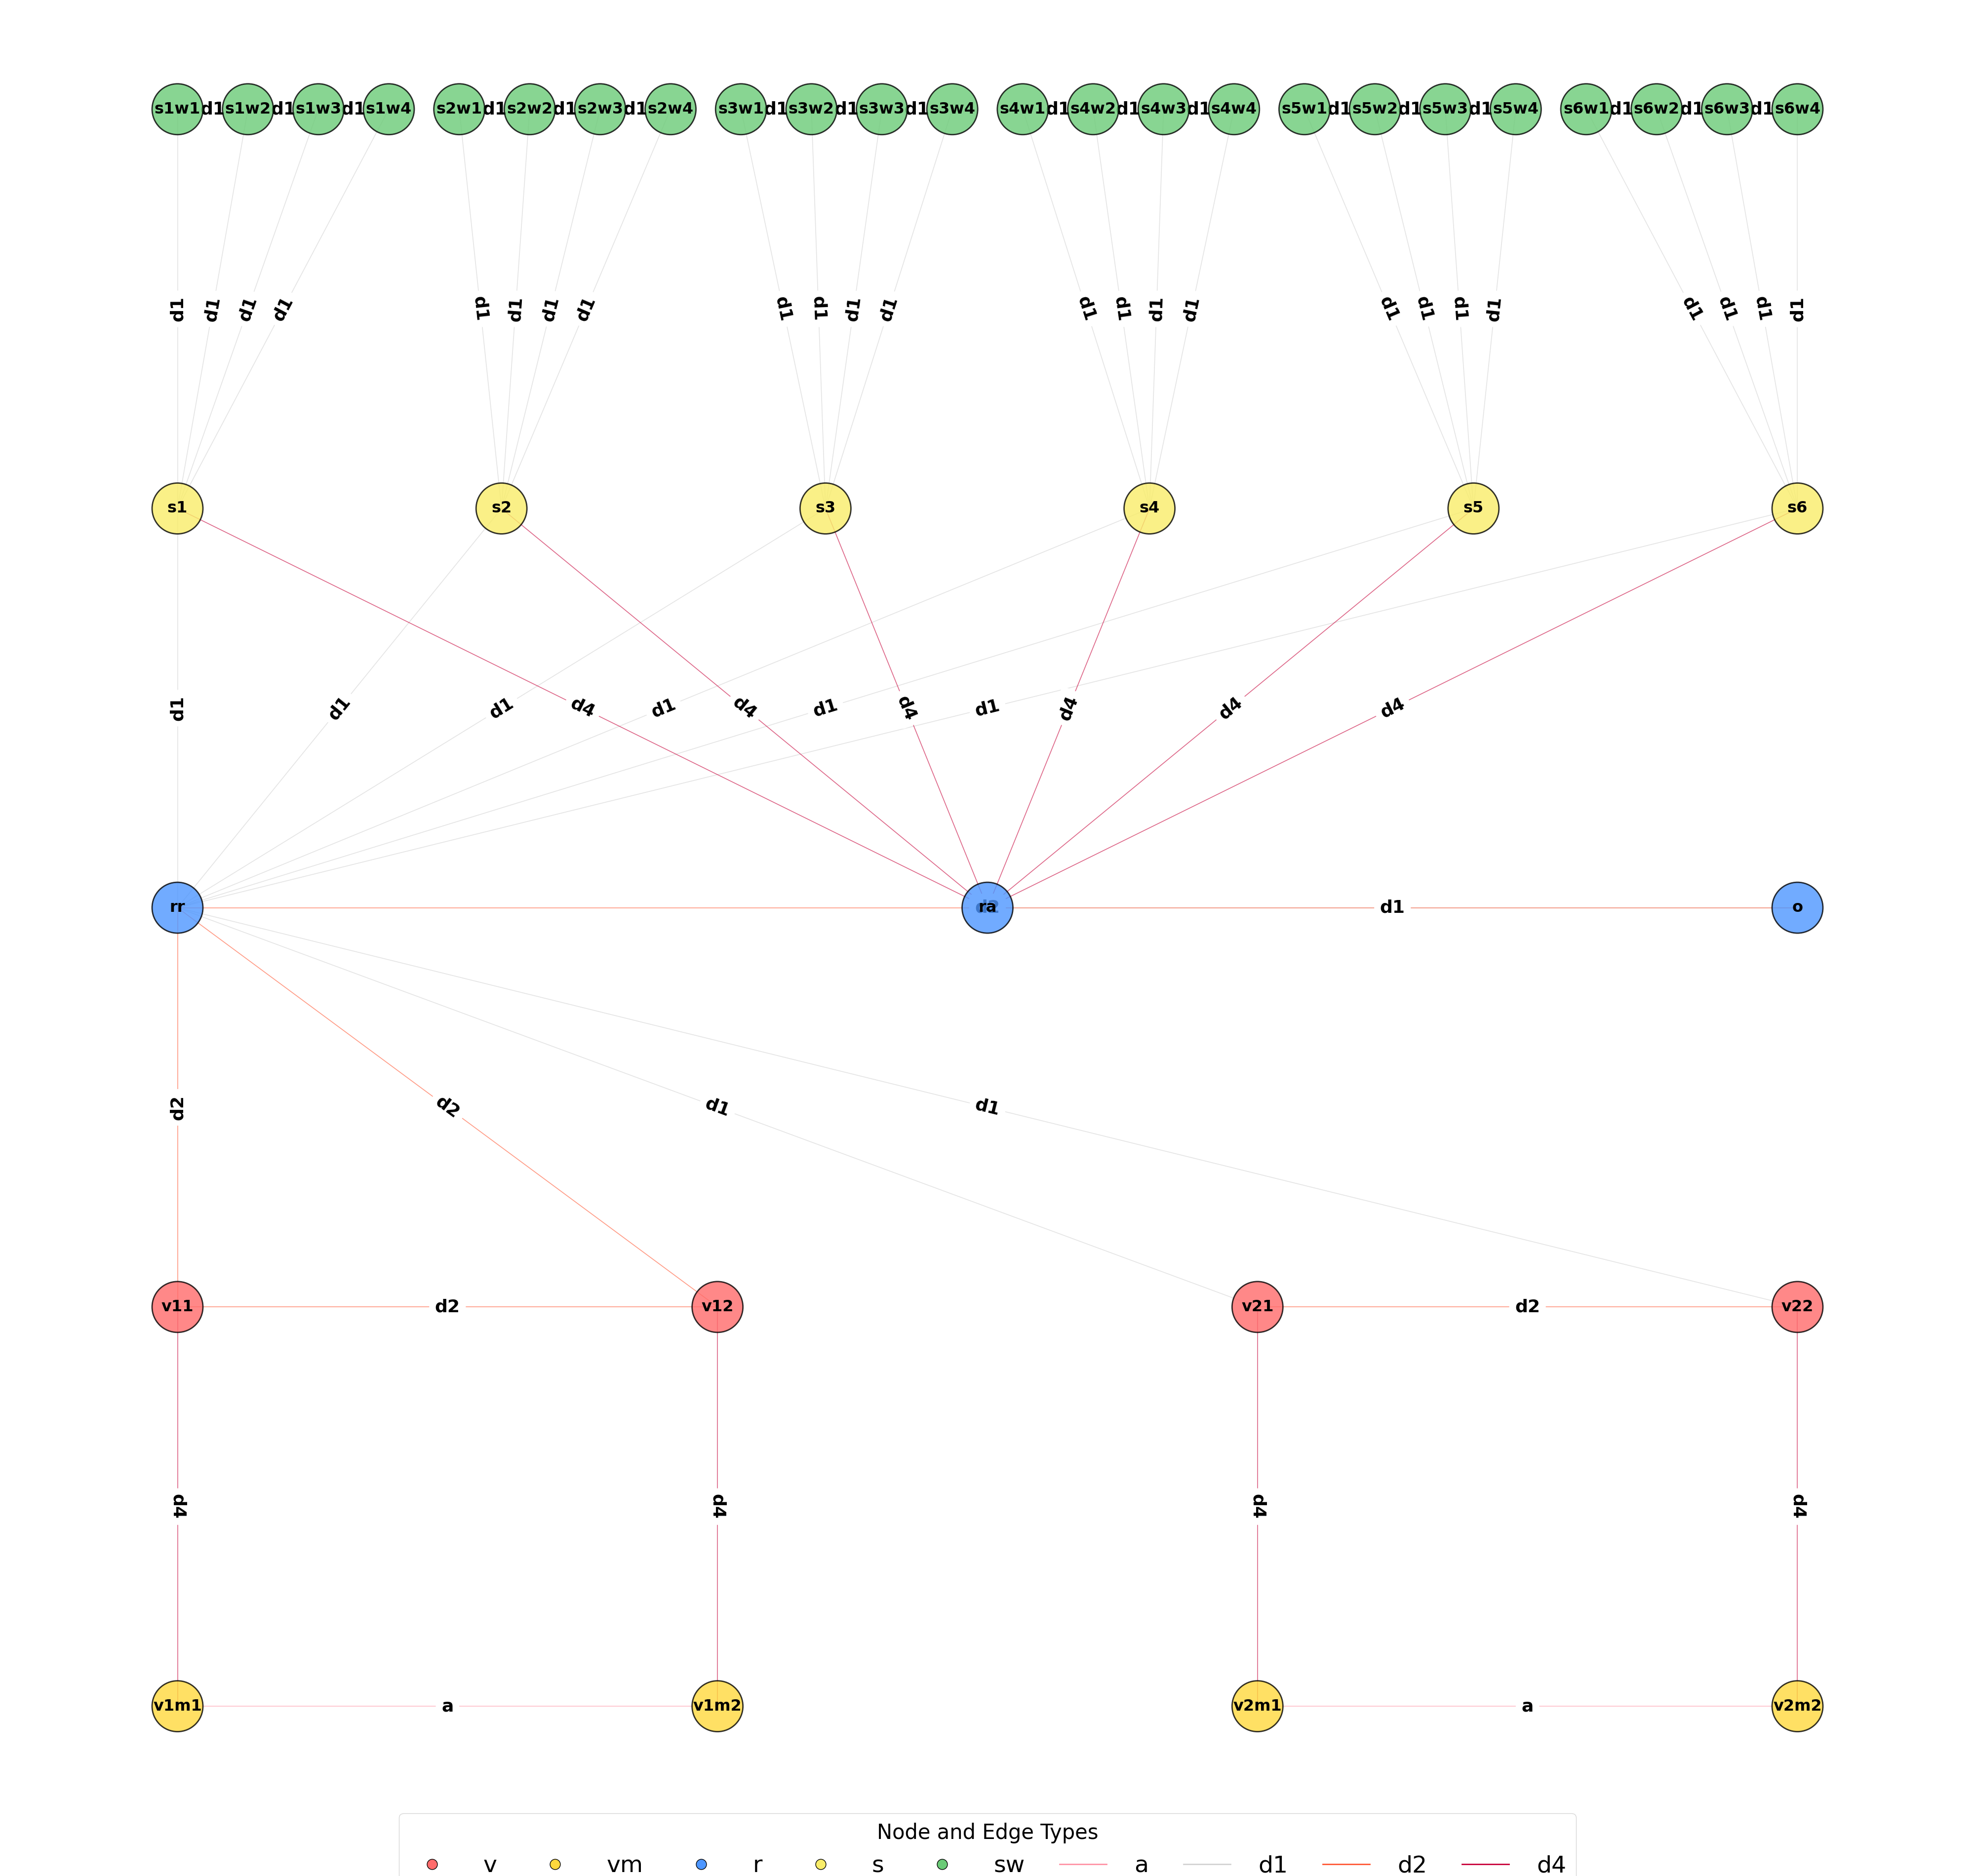
\includegraphics[width=1\textwidth]{./ReportImages/graph.png} 
    \caption{HetGraph}
    \label{fig:HetGraph}
\end{figure}
The count of certain parameters within the motor such as stator poles with its corresponding stator windings and rotor magnets is made more comprehendable to the 
model having new nodes and edges whereas for the \ac{MLP} architecture this information is represented as yet another number in a separate column. \\
By leveraging the relational features introduced by the meta relations, we can obtain a good graph representation of the data.\\

We then learn the constructed heterogeneous graph through a heterogeneous \ac{GNN} model.\\   

Furthermore, we presume graph representation of the data will be more logical than tabular representation due to its ability to grasp the connections within the \ac{EM} structural properties better.
This would be even more realistic with achieving topology invariance than the tabular representation and conserve memory and compute in the long run.
However, we realize that our problem cannot be solved using Homogeneous \ac{GNN} which is relatively simpler and is built on a single node and edge type.
In order to model our problem as a graph, we need to represent it as a Heterogeneous graph. \\

\ac{GNN}s are relatively more expressive models as they can acapture the variability and complexity of our data better.\\
However, \ac{GNN} in general have not been to less explored even so more the heterogeneous \ac{GNN}.
Particularly in the scenario of \ac{EM} Modelling, there has been no publications with \ac{GNN}s.
Hence the need to check its feasibility and its performance with our benchmarks on tabular data.
Additionally, existing Heterogeneous \ac{GNN}s works e.g on recommendation networks, academic networks, information networks, social networks etc involves one large graph with multiple node and edge types. 
However, our problem involves creation of multiple heterogeneous graphs ie, 1 per \ac{EM} variant.\\
Therefore, the applicability of Heterogeneous \ac{GNN}s for our problem is to be seen.

Our thesis is loosely inspired from \cite{ML HGNN-2023} which has strived to extend \ac{MP} into Heterogeneous \ac{GNN}s.\\

\newpage 

\chapter{Conclusion}

This thesis offers a fresh outlook to the possibility of modelling the performance of an \ac{EM} using \ac{GNN}s.
We have developed a topology invariant \ac{MLP} model to predict 2 \ac{KPI}'s of an \ac{EM} from its parameteric requirements. 
It would be very beneficial to \ac{EM} manufacturers to understand the operating range of the vehicle using the motor and make calculated assumptions of whether to manufacture it.\\
This work enables \ac{EM} designers to generate \ac{KPI}'s at almost both negligible costs and minimal time.
Thus offering an escape from the cons of using \ac{FEA} simulations. It also exhibits almost close accuracy to \ac{FEA} simulations with significantly better run time efficiency PROVE\\
It also lays the foundation for future work on being able to generate electric motor design parameters conditioned on the 2 KPIs we predicted.
We envision that our study will provide new perspectives to researchers engaging in the field of electric motor design and hope our contribution will aid in the same.\\
\section{Future Improvements}\label{sec:Future Improvements}

I would suggest the following improvements to our study : 

\begin{enumerate}
    \item Build a model that uses the Torque \ac{KPI} prediction to predict its corresponding Efficiency \ac{KPI}. 
    \item Although we have designed the model to be topology invariant for 3 topologies, we only had sufficient data from Double V Topology to draw evaluations from.
    Further evaluations on the other topologies would be beneficial to critically assess our model's performance.
    \item Another interesting study would be to benchmark model performance when one backpropagates the losses for each \ac{KPI} individually rather than weighing them.
    \item Additionally, the motivation of building a topology invariant model was the reason we have considered building a heterogeneous graph to model the data. The machinery is elaborated in Section \ref{sec:EM Heterogeneous GNN Model}.
    Such a model could serve as yet another ablation study to our problem.
\end{enumerate}

\newpage 

\appendix
\chapter{Appendix}
Supplementary material to the thesis.

\section{Dataset Supplementary Information}
\label{sec:Dataset Supplementary Information}
\subsection{File structure}
\label{subsec:File structure}
Among the excel files shared by Valeo per \ac{EM} variant, table \ref{tab:Excel File Structure} summarizes the sheets of interest to us.
This is helpful for reproducing the experiments, visualizing the Figures \ref{fig:Torque Curve} and \ref{fig:Efficiency Grid} and for carrying out further analysis 
with the same dataset in the future.

\begin{table}[H]
    \centering
    \begin{tabular}{|p{1.7cm}|p{1.5cm}|p{1.3cm}|p{.7cm}|p{8.3cm}|}
    \hline
    {\bf Sheet} & {\bf Sheet Name} & {\bf Plotting Axis} & {\bf Unit} &  {\bf Description}\\
    \hline
    Motor Parameters & input\_data & - & mm, $^\circ$ & Includes geometric, physical and simulation properties.\\
    Speed Grid & NN & x-axis & rpm & Used for plotting the Torque \ac{KPI} and Efficiency \ac{KPI}.\\
    Torque Grid & MM & y-axis & Nm & Used for plotting the Efficiency \ac{KPI}.\\
    Efficiency Grid & ETA & z-axis & - & Has the same dimensions as in NN and MM. \\
    Torque Curve & Mgrenz & y-axis & Nm & Has the same columns as in NN. \\
    \hline
    \end{tabular}
    \caption{Excel File Structure of an \ac{EM} variant}
    \label{tab:Excel File Structure}
\end{table}

\subsection{Data Summary Statistics}
\label{subsec:Data Summary Statistics}

Table \ref{tab:Input Parameters} shows the summary statistics of the input parameters of the motor. 

%Median a column??
\begin{longtable}{|p{1.75cm}|p{0.75cm}|p{1.8cm}|p{1.8cm}|p{3.10cm}|p{1cm}|p{1cm}|p{1cm}|}

    \hline
    \textbf{Parameter} & \textbf{Unit} & \textbf{Mean} & \textbf{Standard Deviation} & \textbf{Value Range} & \textbf{Single V Magnet Topology} & \textbf{Double V Magnet Topology} & \textbf{Nabla Magnet Topology}\\
    \hline
    \endfirsthead
    
    \multicolumn{8}{c}%
    {{\bfseries \tablename\ \thetable{} -- continued from previous page}} \\
    \hline
    \textbf{Parameter} & \textbf{Unit} & \textbf{Mean} & \textbf{Standard Deviation} & \textbf{Value Range} & \textbf{Single V Magnet Topology} & \textbf{Double V Magnet Topology} & \textbf{Nabla Magnet Topology}\\
    \hline
    \endhead

    \hline \multicolumn{8}{|r|}{{Continued on next page}} \\ \hline
    \endfoot

    \hline
    \endlastfoot
    \multicolumn{8}{|l|}{\textbf{General Parameters}} \\
    \hline
    N & - & 4 & 0 & 4 --4  & \checkmark  & \checkmark & \checkmark  \\
    simQ & - & 6 & 0 & 6 -- 6 & \checkmark  & \checkmark  & \checkmark \\
    r\_a & mm & $9\times 10^{-2}$ & $2.5\times 10^{-15}$ & $9\times 10^{-2}$ -- $9\times 10^{-2}$ & \checkmark  & \checkmark  & \checkmark  \\
    r\_i & mm & $6.4433\times 10^{-2}$ & $9.02\times 10^{-4}$ & $6.4 \times 10^{-2}$ -- $6.7\times 10^{-2}$ & \checkmark  & \checkmark  & \checkmark  \\
    \hline
    \multicolumn{8}{|l|}{\textbf{Rotor Parameters}} \\
    \hline
    rad\_phiv2 & rad & -0.5 & $6.36\times 10^{-2}$ & -0.6 -- 0 & $\times$  & \checkmark & $\times$  \\
    lmsov2 & mm & $-2.8\times 10^{-4}$ & $3.5\times 10^{-5}$ &  $-3\times 10^{-4}$ -- 0 & $\times$  & \checkmark & $\times$  \\
    lth1v2 & mm & $5.39\times 10^{-3}$ & $3.5\times 10^{-4}$ & 0 -- $5.45\times 10^{-3}$ & $\times$  & \checkmark & $\times$  \\
    lth2v2 & mm & $2.78\times 10^{-3}$ & $1.7\times 10^{-4}$ & 0 -- $2.8\times 10^{-3}$ & $\times$  & \checkmark & $\times$ \\
    r1v2 & mm & $2.09\times 10^{-3}$ & $3.22\times 10^{-4}$ & 0 -- $2.2\times 10^{-3}$ & $\times$  & \checkmark & $\times$  \\
    r11v2 & mm & $3.26\times 10^{-4}$ & $4\times 10^{-5}$ & 0 -- $6\times 10^{-4}$ & $\times$ &\checkmark & $\times$  \\
    r2v2 & mm & $1.8\times 10^{-3}$ & $1.33\times 10^{-4}$ & 0 -- $1.9\times 10^{-3}$ & $\times$  & \checkmark & $\times$  \\
    r3v2 & mm & $6.97\times 10^{-4}$ & $4.4\times 10^{-5}$ & 0 -- $7\times 10^{-4}$ & $\times$  & \checkmark & $\times$  \\
    r4v2 & mm &  $7.47\times 10^{-4}$ & $4.8\times 10^{-5}$ & 0 -- $7.5\times 10^{-4}$ & $\times$  & \checkmark & $\times$  \\
    rmt1v2 & mm & $2.49\times 10^{-4}$ & $1.6\times 10^{-5}$ & 0 -- $2.5\times 10^{-4}$ & $\times$  & \checkmark &$\times$  \\
    rmt4v2 & mm & $2.49\times 10^{-4}$ & $1.6\times 10^{-5}$ & 0 -- $2.5\times 10^{-4}$ & $\times$  & \checkmark & $\times$  \\
    rlt1v2 & mm & $1.85\times 10^{-4}$ &  $4.5\times 10^{-5}$ & 0 -- $2\times 10^{-4}$ & $\times$  & \checkmark & $\times$  \\
    rlt4v2 & mm & $2.49\times 10^{-4}$ & $1.6\times 10^{-5}$ & 0 -- $2.5\times 10^{-4}$ & $\times$ & \checkmark & $\times$ \\
    hav2 & mm & $4.9\times 10^{-3}$ & $3.36\times 10^{-4}$ &  0 -- $5\times 10^{-3}$ & $\times$  & \checkmark & $\times$  \\
    mbv2 & mm & $1.7\times 10^{-2}$ & $1.17\times 10^{-3}$ & 0 -- $1.8\times 10^{-2}$ & $\times$  & \checkmark & $\times$  \\
    mhv2 & mm & $3.6\times 10^{-3}$ & $2.65\times 10^{-4}$ & 0 -- $3.8\times 10^{-3}$ & $\times$ &\checkmark & $\times$  \\
    rmagv2 & mm & $4.98\times 10^{-4}$ & $3.2\times 10^{-5}$ & 0 -- $5\times 10^{-4}$ & $\times$  & \checkmark & $\times$  \\
    dsmv2 & mm & $2.9\times 10^{-3}$ & $1.9\times 10^{-4}$ & 0 -- $3.1\times 10^{-3}$ & $\times$  & \checkmark & $\times$ \\
    dsmuv2 & mm & $2.9\times 10^{-3}$ & $1.9\times 10^{-4}$ & 0 -- $3.1\times 10^{-3}$ & $\times$  & \checkmark & $\times$  \\
    amtrv2 & mm & $1.58\times 10^{-2}$ & $1.024\times 10^{-3}$ & 0 -- $1.6\times 10^{-2}$ & $\times$  & \checkmark & $\times$ \\
    dsrv2 & mm & $9.96\times 10^{-4}$ & $6.4\times 10^{-5}$ & 0 -- $1\times 10^{-3}$ & $\times$  & \checkmark & $\times$ \\
    lmav2 & mm & $1\times 10^{-4}$ & $3\times 10^{-5}$ & 0 -- $1.1\times 10^{-4}$ & $\times$  & \checkmark & $\times$  \\
    lmiv2 & mm & $1.09\times 10^{-4}$ & $8\times 10^{-6}$ & 0 -- $1.10\times 10^{-4}$ & $\times$  & \checkmark & $\times$  \\
    lmov2 & mm & $5.5\times 10^{-5}$ & $1.5\times 10^{-5}$ & 0 -- $1\times 10^{-4}$ & $\times$  & \checkmark & $\times$  \\
    lmuv2 & mm & $1.45\times 10^{-4}$ & 10 & 0 -- $1.5\times 10^{-4}$ & $\times$  & \checkmark & $\times$ \\
    rad\_phiv1 & rad & -$6.9\times 10^{-1}$ & $5.4\times 10^{-2}$ & -$7.8\times 10^{-1}$ -- -$4.5\times 10^{-1}$ &\checkmark & \checkmark & \checkmark\\
    lmsov1 & mm & -$5.01\times 10^{-4}$ & $9.4\times 10^{-5}$ & -$5.3\times 10^{-4}$ -- $5\times 10^{-4}$ &\checkmark & \checkmark & \checkmark\\
    lth1v1 & mm & $2.8\times 10^{-3}$ & $1.7\times 10^{-4}$ & $2.8\times 10^{-3}$ -- $5.45\times 10^{-3}$ &\checkmark & \checkmark & \checkmark\\
    lth2v1 & mm & $2.104\times 10^{-3}$ & $5.9\times 10^{-5}$ & $2.1\times 10^{-3}$ -- $3.2\times 10^{-3}$ &\checkmark & \checkmark & \checkmark\\
    r1v1 & mm & $4.07\times 10^{-4}$ & $1.08\times 10^{-4}$ & $4\times 10^{-4}$ -- $2.2\times 10^{-3}$ &\checkmark & \checkmark & \checkmark\\
    r11v1 & mm & $2.19\times 10^{-4}$ & $4.5\times 10^{-5}$ & $1\times 10^{-4}$ -- $6\times 10^{-4}$ &\checkmark & \checkmark & \checkmark\\
    r2v1 & mm & $2.16\times 10^{-4}$ & $1\times 10^{-4}$ & $2\times 10^{-4}$ -- $1.9\times 10^{-3} $&\checkmark & \checkmark & \checkmark\\
    r3v1 & mm & $8.99\times 10^{-4}$ & $1.3\times 10^{-5}$ & $7\times 10^{-4}$ -- $9\times 10^{-4}$ &\checkmark & \checkmark & \checkmark\\
    r4v1 & mm & $5.01\times 10^{-4}$ & $1.6\times 10^{-5}$ & $5\times 10^{-4}$ -- $7.5\times 10^{-4}$ &\checkmark & \checkmark & \checkmark\\
    rmt1v1 & mm & $2.5\times 10^{-4}$ & $8.8\times 10^{-18}$ & $2.5\times 10^{-4}$ -- $2.5\times 10^{-4}$ &\checkmark & \checkmark & \checkmark\\
    rmt4v1 & mm & $2.5\times 10^{-4}$ & $8.8\times 10^{-18}$ & $2.5\times 10^{-4}$ -- $2.5\times 10^{-4} $&\checkmark & \checkmark & \checkmark\\
    rlt1v1 & mm & $1.17\times 10^{-4}$ & $5.6\times 10^{-5} $& $5\times 10^{-5}$ -- $2.5\times 10^{-4}$ &\checkmark & \checkmark & \checkmark\\
    rlt4v1 & mm & $2.5\times 10^{-4}$ & $8.8\times 10^{-18}$ & $2.5\times 10^{-4}$ --$ 2.5\times 10^{-4}$ &\checkmark & \checkmark & \checkmark\\
    hav1 & mm & $2.9\times 10^{-3}$ & $1.36\times 10^{-4}$ & $2.9\times 10^{-3} $-- $5\times 10^{-3}$ &\checkmark & \checkmark & \checkmark\\
    mbv1 & mm & $7.6\times 10^{-3}$ & $5.8\times 10^{-4}$ & $7.5\times 10^{-3}$ -- $1.8\times 10^{-2}$ &\checkmark & \checkmark & \checkmark\\
    mhv1 & mm & $2.8\times 10^{-3}$ & $1.4\times 10^{-4}$ & $2.7\times 10^{-3}$ -- $5\times 10^{-3}$ &\checkmark & \checkmark & \checkmark\\
    rmagv1 & mm & $5\times 10^{-4}$ & $1.7\times 10^{-17}$ & $5\times 10^{-4}$ -- $5\times 10^{-4}$ &\checkmark & \checkmark & \checkmark\\
    dsmv1 & mm & $1.07\times 10^{-3}$ & $1.41\times 10^{-4}$ & $8\times 10^{-4}$ -- $2.8\times 10^{-3}$ &\checkmark & \checkmark & \checkmark\\
    dsmuv1 & mm & $1.07\times 10^{-3}$ & $1.47\times 10^{-4}$ & $8\times 10^{-4}$ -- $2.92\times 10^{-3}$ &\checkmark & \checkmark & \checkmark\\
    amtrv1 & mm & $5.5\times 10^{-3}$ & $6.34\times 10^{-4}$ & $5.5\times 10^{-3}$ -- $1.9\times 10^{-2}$ &\checkmark & \checkmark & \checkmark\\
    dsrv1 & mm & $7.5\times 10^{-4}$ & $3.2\times 10^{-5}$ & $7.5\times 10^{-4}$ -- $1.25\times 10^{-3}$ &\checkmark & \checkmark & \checkmark\\
    lmav1 & mm & $9.2\times 10^{-5}$ & $2.6\times 10^{-5}$ & $1\times 10^{-5}$ -- $1.1\times 10^{-4}$ &\checkmark & \checkmark & \checkmark\\
    lmiv1 & mm & $1\times 10^{-4}$ & $6.35\times 10^{-7}$ & $1\times 10^{-4}$ -- $1.1\times 10^{-4} $&\checkmark & \checkmark & \checkmark\\
    lmov1 & mm & $5.5\times 10^{-5}$ & $1.5\times 10^{-5}$ & $5\times 10^{-5}$ -- $1\times 10^{-4}$ &\checkmark & \checkmark & \checkmark\\
    lmuv1 & mm & $1.45\times 10^{-4}$ & $1.5\times 10^{-5}$ & $1\times 10^{-4}$ -- $1.5\times 10^{-4}$ &\checkmark & \checkmark & \checkmark\\
    rad\_phi3b1 & rad & - $2.5\times 10^{-3}$ & $5.6001\times 10^{-2}$ & -1.25 -- 0 & $\times$  & $\times$  & \checkmark  \\
    rad\_phi4b1 & rad & -$5.3\times 10^{-4}$ & $1.1775\times 10^{-2}$ & -0.26 -- 0  & $\times$  & $\times$  & \checkmark  \\
    lmsob1 & mm & $2\times 10^{-6}$ & $3.4\times 10^{-5}$ & 0 -- $7.5\times 10^{-4}$ & $\times$  & $\times$  & \checkmark  \\
    lthb1 & mm & $6\times 10^{-6}$ & $1.28\times 10^{-4}$ & 0 -- $2.9\times 10^{-3}$ & $\times$  & $\times$  & \checkmark  \\
    r2b1 & mm & $2\times 10^{-6}$ & $4.5\times 10^{-5}$ & 0 -- $1\times 10^{-3}$ & $\times$  & $\times$  & \checkmark  \\
    r3b1 & mm & $2\times 10^{-6}$ & $3.4\times 10^{-5}$ & 0 -- $1\times 10^{-3}$ & $\times$  & $\times$  & \checkmark  \\
    r4b1 & mm & $5.06\times 10^{-7}$& $1.1\times 10^{-5}$ & 0 -- $2.5\times 10^{-4}$ & $\times$  & $\times$  & \checkmark  \\
    r5b1 & mm & $5.06\times 10^{-7}$ & $1.1\times 10^{-5}$ & 0 -- $2.5\times 10^{-4} $& $\times$  & $\times$  & \checkmark  \\
    lgr3b1 & mm & $1\times 10^{-6}$ & $2.2\times 10^{-5}$ & 0 -- $5\times 10^{-4}$ & $\times$  & $\times$  & \checkmark  \\
    lgr4b1 & mm & $6.07\times 10^{-7}$ & $1.3\times 10^{-5}$ & 0 -- $3\times 10^{-4}$ & $\times$  & $\times$  & \checkmark  \\
    mbb1 & mm & $3\times 10^{-5}$ & $6.75\times 10^{-4}$ & 0 -- $1.5\times 10^{-2}$ & $\times$ & $\times$  & \checkmark \\
    mhb1 & mm & $6\times 10^{-6}$ & $1.4\times 10^{-4}$ & 0 -- $3.2\times 10^{-3}$ & $\times$  & $\times$ & \checkmark \\
    mtbb1 & mm & $3\times 10^{-5}$ & $6.75\times 10^{-4}$ & 0 -- $1.5\times 10^{-2}$ & $\times$  &$\times$ & \checkmark  \\
    rmagb1 & mm & $1\times 10^{-6}$ & $2.2\times 10^{-5}$ & 0 -- $5\times 10^{-4}$ & $\times$  & $\times$ & \checkmark \\
    amtrb1 & mm & $4\times 10^{-6}$ & $9.8\times 10^{-5}$ & 0 -- $2.5\times 10^{-3}$ & $\times$  & $\times$  & \checkmark  \\
    dsr3b1 & mm & $3\times 10^{-6}$ & $6.6\times 10^{-5}$ & 0 -- $1.85\times 10^{-3}$ & $\times$ & $\times$ & \checkmark  \\
    dsr4b1 & mm & $4\times 10^{-6}$ & $8.3\times 10^{-5}$ & 0 -- $1.85\times 10^{-3}$ & $\times$  & $\times$  & \checkmark \\
    lmob1 & mm & $2.02\times 10^{-7}$ & $4.49\times 10^{-6}$ & 0 -- $1\times 10^{-4}$ & $\times$  & $\times$ & \checkmark \\
    lmub1 & mm & $3.03\times 10^{-7}$ & $6.7\times 10^{-6}$ & 0 -- $1.5\times 10^{-4}$ & $\times$  & $\times$  & \checkmark \\
    lmsub1 & mm & $4\times 10^{-6}$ & $8.1\times 10^{-5}$ & 0 -- $1.8\times 10^{-3}$ &$\times$  & $\times$  & \checkmark \\
    \hline
    \multicolumn{8}{|l|}{\textbf{Stator Parameters}} \\
    \hline
    airgap & mm & $1\times 10^{-3}$ & $3.5\times 10^{-17}$ & $1\times 10^{-3}$ -- $1\times 10^{-3}$ &\checkmark  & \checkmark  & \checkmark  \\
    b\_nng & mm & $5.04\times 10^{-3}$ & $9.1\times 10^{-5}$ & $4.6\times 10^{-3}$ -- $5.1\times 10^{-3}$ & \checkmark  & \checkmark  & \checkmark  \\
    b\_nzk & mm & $4.5\times 10^{-3}$ & $5.7\times 10^{-5}$ & $4.45\times 10^{-3}$ -- $4.6\times 10^{-3}$ & \checkmark  & \checkmark  & \checkmark  \\
    b\_s & mm & $1\times 10^{-3}$ & $2.5\times 10^{-5}$ & $1\times 10^{-3}$ -- $1.4\times 10^{-3}$ & \checkmark  & \checkmark  & \checkmark  \\
    h\_n & mm & $1.1\times 10^{-2}$ & $8.06\times 10^{-4}$ & $9.2\times 10^{-3}$ -- $1.39\times 10^{-2}$ & \checkmark  & \checkmark  & \checkmark  \\
    h\_s & mm & $1\times 10^{-3}$ & $3.5\times 10^{-17}$& $1\times 10^{-3}$ -- $1\times 10^{-3}$ & \checkmark  & \checkmark  & \checkmark  \\
    r\_sn & mm & $2.5\times 10^{-4}$ & $8.8\times 10^{-18}$ & $2.5\times 10^{-4}$ -- $2.5\times 10^{-4}$ & \checkmark  & \checkmark  & \checkmark  \\
    r\_zk & mm & $5.01\times 10^{-4}$ & $1.9\times 10^{-5}$ & $5\times 10^{-4}$ -- $8\times 10^{-4}$ & \checkmark  & \checkmark  & \checkmark  \\
    r\_ng & mm & $5.01\times 10^{-4}$ & $1.9\times 10^{-5}$ & $5\times 10^{-4}$ -- $8\times 10^{-4}$ & \checkmark  & \checkmark  & \checkmark  \\
    h\_zk & mm & $1\times 10^{-3}$ & $3.5\times 10^{-17}$ & $1\times 10^{-3}$ -- $1\times 10^{-3}$ & \checkmark  & \checkmark  & \checkmark  \\
    bhp & mm & $3.7\times 10^{-3}$ & $8.1\times 10^{-5}$ & $3.5\times 10^{-3}$ -- $3.8\times 10^{-3}$ &\checkmark  & \checkmark  & \checkmark  \\
    hhp & mm & $2.38\times 10^{-3}$ & $1.9\times 10^{-4}$ & $1.9\times 10^{-3}$ -- $2.8\times 10^{-3}$ &\checkmark  & \checkmark  & \checkmark  \\
    rhp & mm & $6.36\times 10^{-4}$ & $4.5\times 10^{-5}$ & $5\times 10^{-4}$ -- $8\times 10^{-4}$ &\checkmark  & \checkmark  & \checkmark  \\
    dhphp & mm & $2.6\times 10^{-4}$ & $1.4\times 10^{-5}$ & $2.6\times 10^{-4}$ -- $4.8\times 10^{-4}$ &\checkmark  & \checkmark  & \checkmark  \\
    dhpng & mm & $4.06\times 10^{-4} $& $3\times 10^{-6}$ & $4.06\times 10^{-4}$ -- $4.5\times 10^{-4} $&\checkmark  & \checkmark  & \checkmark  \\
    \hline
    \caption{\ac{EM} Input Parameters}
    \label{tab:Input Parameters} \\
\end{longtable}

It gives us a clear idea of how the parameters of the Rotor can vary across Topologies.
In addition the \textit{N} and \textit{simQ} parameters are count of Stator poles and its windings respectively and may vary across \ac{EM} variants.\\
1481 examples are of the Double V Magnet Topology apart from which 3 examples each for the other 2 topologies.
Hence, the imbalanced topologies parameters would have relatively not so reliable statistics.\\ 

\section{Experimental setup}
\label{sec:Experimental setup}

\begin{figure}[H]
    \centering
    \begin{subfigure}{0.32\textwidth}
        \centering
        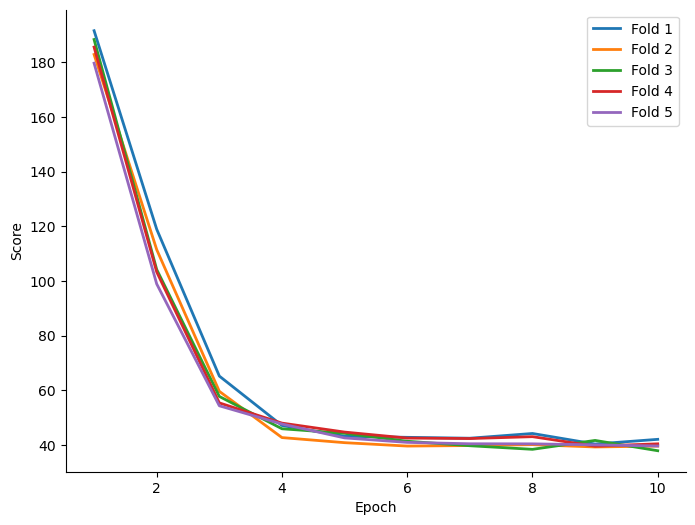
\includegraphics[width=\textwidth]{./ReportImages/train_score.png}
        \caption{\centering Aggregated Training Score}
        \label{fig:Aggregated Training Score}
    \end{subfigure}\hfill
    \begin{subfigure}{0.32\textwidth}
        \centering
        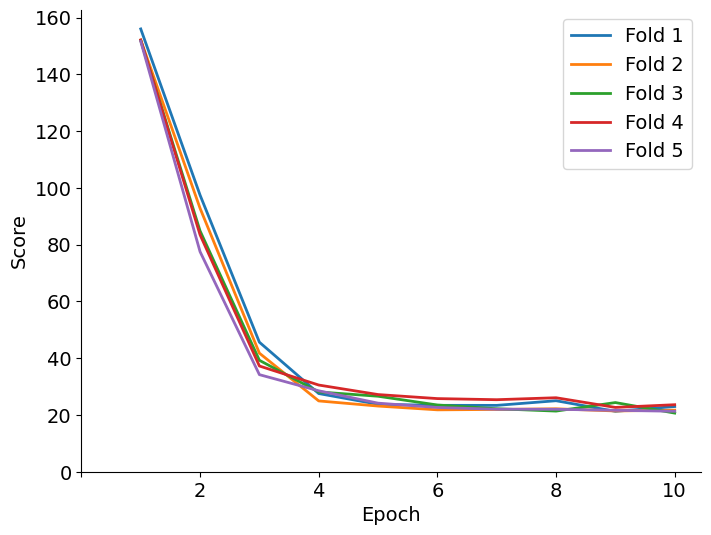
\includegraphics[width=\textwidth]{./ReportImages/train_score_y1.png}
        \caption{\centering Training Score for Torque \ac{KPI}}
        \label{fig:Training Score for Torque Curve}
    \end{subfigure}\hfill
    \begin{subfigure}{0.32\textwidth}
        \centering
        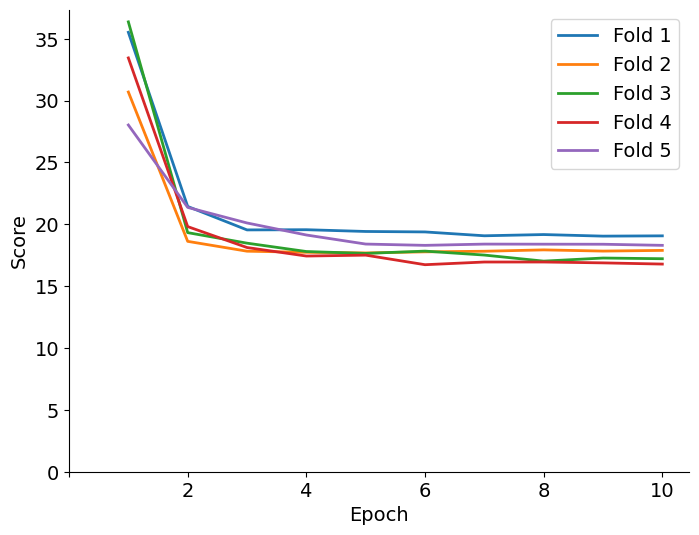
\includegraphics[width=\textwidth]{./ReportImages/train_score_y2.png}
        \caption{\centering Training Score for Efficiency \ac{KPI}}
        \label{fig:Training Score for Efficiency grid}
    \end{subfigure}
    \caption{Training Evaluation Metrics}
    \label{fig:Training Evaluation Metrics}
\end{figure}

\begin{figure}[H]
    \centering
    \begin{subfigure}{0.32\textwidth}
        \centering
        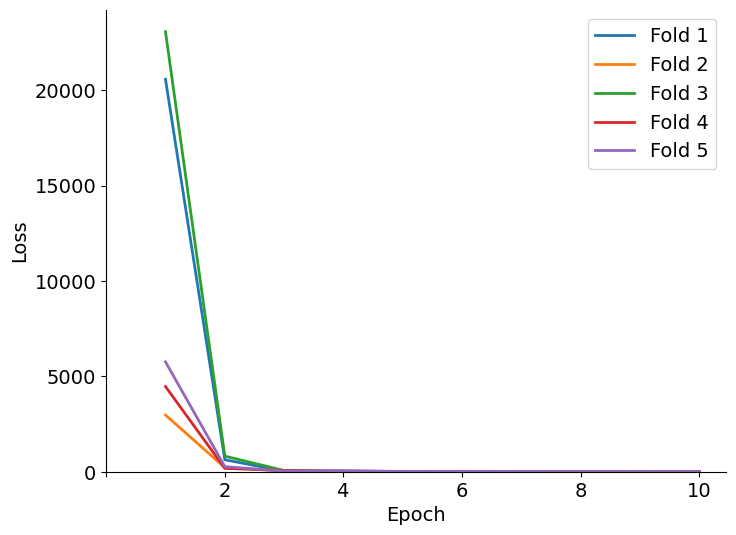
\includegraphics[width=\textwidth]{./ReportImages/val_loss.png}
        \caption{\centering Aggregated Validation Loss}
        \label{fig:Aggregated Validation Loss}
    \end{subfigure}\hfill
    \begin{subfigure}{0.32\textwidth}
        \centering
        \includegraphics[width=\textwidth]{./ReportImages/val_loss_y1.png}
        \caption{\centering Validation Loss for Torque \ac{KPI}}
        \label{fig:Validation Loss for Torque Curve}
    \end{subfigure}\hfill
    \begin{subfigure}{0.32\textwidth}
        \centering
        \includegraphics[width=\textwidth]{./ReportImages/val_loss_y2.png}
        \caption{\centering Validation Loss for Efficiency \ac{KPI}}
        \label{fig:Validation Loss for Efficiency grid}
    \end{subfigure}
    \caption{Validation Loss Metrics}
    \label{fig:Validation Loss Metrics}
\end{figure}

\section{GNN Terminologies}
\label{sec:GNN Terminologies}

We largely adopt the commonly used notations from \cite{GNN-2019} and reformulate it slightly to meet our needs.
We use bold uppercase characters to denote matrices and bold lowercase characters to denote vectors.\\

\textbf{Graphs}

A graph is represented as \( \mathcal{G} = (V, E) \) where \( V \) is the set of vertices or nodes  and \( E \) is the set of edges. 
Let \( v_i \in V \) denote a node and \( e_{ij} = (v_i, v_j) \in E \) denote an edge pointing from \( v_j \) to \( v_i \).
A graph may have node attributes \( X \), where \( X \in \mathbb{R}^{n \times d} \) is a node feature matrix with 
\( x_v \in \mathbb{R}^d \) representing the feature vector of a node \( v \). 
Meanwhile, a graph may have edge attributes \( X_e \), where \( X_e \in \mathbb{R}^{m \times \\c} \) is an edge
feature matrix with \( x_{v,u} \in \mathbb{R}^c \) representing the feature vector of an edge \( (v, u) \).\\

\textbf{Neighbourhood}

Neighbourhood essentially holds the information of the set of nodes that are in the vicinitY of a node in question.
The neighborhood of a node \( v \) is defined as \( N(v) = \{ u \in V \mid (v, u) \in E \} \).\\

\textbf{Adjacency Matrix}

Adjacency matrix gives an overview of the neighbourhood of all nodes in the graph. It is typically referenced when performing \ac{MP} algorithm.
The adjacency matrix \( A \) is a \( n \times n \) matrix with \( A_{ij} = 1 \) if \( e_{ij} \in E \) and \( A_{ij} = 0 \) if \( e_{ij} \notin E \).\\

\textbf{Diagonal Matrix} 

Diagonal Matrix of \( A \) denoted by  \( D = \operatorname{diag}(d_1, d_2, \dots, d_n) \), where \( d_i = \sum_{j} a_{ij} \) is the degree of vertex \( i \).\\

\textbf{Laplacian Matrix}

The graph Laplacian is defined as \( L := D - A \) \\ and the normalized Adjacency Matrix can be defined as
\[
A_{\text{norm}} = D^{-\frac{1}{2}} A D^{-\frac{1}{2}}.
\]

\textbf{Reference Operator}

The Reference Operator \( R \) is a matrix of the same sparsity as the Adjacency Matrix \( A \). It is also called as Structure or Graph Shift operator.\\

\textbf{Transformation Operator}

The Transformation Operator is a feature map or a learnable matrix of weights, \( \theta \in \mathbb{R}^{F \times F'} \):\\

\textbf{Message Passing}

For Graph signals, \( V = [v_1, v_2, \dots, v_n], v_i  \in \mathbb{R}^F \), the updated Graph Signals is \( V' = RV\theta \) 
where \( RV \) is the weighted sum of graph signals neighbourhood. \( RV \) also ensures only nodes with edges is considered.

In contrast to \ac{CNN}s fixed shape kernel which considers pixels locality we have an increasing shaped kernel for \ac{GNN}s, this is clear in the Figure \ref{fig:GNN Kernel Filter}. 
The fixed shaped kernel does not work for graphs  as they are irregular in size and not constrained to pixel dimensions as images are. 
It is also called a Polynomial Graph Filter or Radial Filter and can be expressed as

\[ V' = \sigma (\sum_{k=0}^{K}R^{k}V\theta^{k}) \]

\begin{figure}[H]
    \centering
    \includegraphics[width=0.6\textwidth]{./ReportImages/GNNKernel.png} 
    \caption{\ac{GNN} Kernel Filter Source :WWW}
    \label{fig:GNN Kernel Filter}
\end{figure}

A \ac{GNN} block contains three update functions, \( \phi \), and three aggregation functions, \( \rho \) for the nodes, edges and graph attributes, \cite{GNNs-2018}
\[
e'_k = \phi_e(e_k, v_{r_k}, v_{s_k}, u)
\]
\[
v'_i = \phi_v(\bar{e}'_i, v_i, u)
\]
\[
u' = \phi_u(\bar{e}', \bar{v}', u)
\]
\[
\bar{e}'_i = \rho_{e \to v}(E'_i)
\]
\[
\bar{e}' = \rho_{e \to u}(E')
\]
\[
\bar{v}' = \rho_{v \to u}(V')
\]


\listoffigures

\newpage 

\listoftables

\newpage 

\begin{thebibliography}{00}

    \bibitem[01]{EHR HGNN-2024}
    \newblock Tsai Hor Chana, Guosheng Yina, Kyongtae Baeb, Lequan Yu 
    \newblock {\em Multi-task Heterogeneous Graph Learning on Electronic Health Records}.
    \newblock cs.LG, 14 Aug 2024.
    
    \bibitem[02]{SE HGNN-2023}
    \newblock Xiaocheng Yang, Mingyu Yan, Shirui Pan, Xiaochun Ye, Dongrui Fan
    \newblock {\em Simple and Efficient Heterogeneous Graph Neural Network}.
    \newblock cs.LG, 1 Sep 2023.

    \bibitem[03]{EV HGNN-2023}
    \newblock Xinru Huang
    \newblock {\em A Heterogeneous Graph Neural Network Model for Electric Vehicle Purchase Propensity Prediction}.
    \newblock ICDSCA, Oct 2023.
    
    \bibitem[04]{REF HGNN-2021}
    \newblock Qingsong Lv, Ming Ding, Qiang Liu, Yuxiang Chen, Wenzheng Feng, Siming He, Chang Zhou, Jianguo Jiang, Yuxiao Dong, Jie Tang
    \newblock {\em Are we really making much progress? Revisiting, benchmarking, and refining heterogeneous graph neural networks}.
    \newblock cs.LG, 30 Dec 2021.

    \bibitem[05]{ML HGNN-2023}
    \newblock Fredrik Johannessen, Martin Jullum
    \newblock {\em Finding Money Launderers Using Heterogeneous Graph Neural Networks}.
    \newblock ICDSCA, 25 July 2023.
    
    \bibitem[06]{PO GNN-2018}
    \newblock Damian Owerko, Fernando Gama, Alejandro Ribeiro
    \newblock {\em Predicting Power Outages Using Graph Neural Networks}.
    \newblock cs.LG, Nov 2018.

    \bibitem[07]{SM EMT-2020}
    \newblock Mikko Tahkola, Janne Keränen, Denis Sedov, Mehrnaz Farzam Far, Juha Kortelainen
    \newblock {\em Surrogate Modeling of Electrical Machine Torque Using Artificial Neural Networks}.
    \newblock ICDSCA, Dec 17 2020.
    
    \bibitem[08]{EM 2DFMP-2022}
    \newblock AKM Khaled Ahsan Talukder, Bingnan Wang and Yusuke Sakamoto
    \newblock {\em Electric Machine Two-dimensional Flux Map Prediction with Ensemble Learning}.
    \newblock ICEMS, 2022.

    \bibitem[09]{T-CNN-2024}
    \newblock Kazuhisa Iwata, Hidenori Sasaki, Hajime Igarashi, Daisuke Nakagawa, and Tomoya Ueda
    \newblock {\em Generalization Performance in Predicting Torque Characteristics Using Convolutional Neural Network and Stator Magnetic Flux.}
    \newblock ICDSCA, 3 Mar 2024.
    
    \bibitem[10]{EM MP-2021}
    \newblock Simone Ferrari, Paolo Ragazzo, Gaetano Dilevrano, Gianmario Pellegrino
    \newblock {\em Flux-Map Based FEA Evaluation of Synchronous Machine Efficiency Maps}.
    \newblock WEMDCD, 2021.

    \bibitem[11]{EM 2DFMP-2021}
    \newblock Vivek Parekh, Dominik Flore, Sebastian Schöps
    \newblock {\em Deep Learning-Based Prediction of Key Performance Indicators for Electrical Machines}.
    \newblock Jan 22, 2021.

    \bibitem[12]{EMAP-2020}
    \newblock Carlos Candelo-Zuluaga, Antonio Garcia Espinosa, Jordi-Roger Riba, Pere Tubert Blanch
    \newblock {\em Computationally Efficient Analysis of Spatial and Temporal Harmonics Content of the Magnetic Flux Distribution in a PMSM for Efficiency Maps Computation.}
    \newblock 2020.
    
    \bibitem[13]{EM SM-2023}
    \newblock Yihao Xu, Bingnan Wang, Yusuke Sakamoto, Tatsuya Yamamoto, and Yuki Nishimura
    \newblock {\em Comparison of Learning-based Surrogate Models for Electric Motors}.
    \newblock COMPUMAG, 2023.

    \bibitem[14]{IM HML-2021}
    \newblock Marius Stender, Oliver Wallscheid, Joachim Böcker
    \newblock {\em Accurate Torque Estimation for Induction Motors by Utilizing a Hybrid Machine Learning Approach}.
    \newblock PEMC, 2021.

    \bibitem[15]{EM CNN-2024}
    \newblock Kazuhisa Iwata, Hidenori Sasaki, Hajime Igarashi, Daisuke Nakagawa, Tomoya Ueda
    \newblock {\em Generalization Performance in Predicting Torque Characteristics Using Convolutional Neural Network and Stator Magnetic Flux}
    \newblock 3 March, 2024.
    
    \bibitem[16]{EM TL-2020}
    \newblock Arbaaz Khan, Mohammad Hossain Mohammadi, Vahid Ghorbanian, David Lowther
    \newblock {\em Transfer Learning for Efficiency Map Prediction}.
    \newblock CEFC, 2020.

    \bibitem[17]{ADAM-2017}
    \newblock Diederik P. Kingma, Jimmy Ba
    \newblock {\em Adam: A Method for Stochastic Optimization}.
    \newblock 30 Jan 2017.

    \bibitem[18]{GNN-2019}
    \newblock Zonghan Wu, Shirui Pan, Fengwen Chen, Guodong Long, Chengqi Zhang, Philip S. Yu
    \newblock {\em A Comprehensive Survey on Graph Neural Networks}.
    \newblock 04 Dec 2019.

    \bibitem[19]{GNNs-2018}
    \newblock Peter W. Battaglia, Jessica B. Hamrick, Victor Bapst, Alvaro Sanchez-Gonzalez, Vinicius Zambaldi, Mateusz Malinowski, Andrea Tacchetti, David Raposo, 
    Adam Santoro, Ryan Faulkner, Caglar Gulcehre, Francis Song, Andrew Ballard, Justin Gilmer, George Dahl, Ashish Vaswani, Kelsey Allen, Charles Nash,
    Victoria Langston, Chris Dyer, Nicolas Heess, Daan Wierstra, Pushmeet Kohli, Matt Botvinick, Oriol Vinyals, Yujia Li, Razvan Pascanu
    \newblock {\em Relational inductive biases, deep learning, and graph networks}.
    \newblock 17 Oct 2018.

    \bibitem[20]{RSHGNN-2019}
    \newblock Shichao Zhu, Chuan Zhou, Shirui Pan, Xingquan Zhu, Bin Wang
    \newblock {\em Relation Structure-Aware Heterogeneous Graph Neural Network}.
    \newblock 2019.

    \bibitem[21]{PR-HGNN-2024}
    \newblock Xingtong Yu, Yuan Fang, Zemin Liu, Xinming Zhang
    \newblock {\em HGPROMPT: Bridging Homogeneous and Heterogeneous Graphs for Few-shot Prompt Learning}.
    \newblock 5 Jan 2024.

    \bibitem[22]{GCN-2018}
    \newblock Qimai Li, Zhichao Han, Xiao-Ming Wu
    \newblock {\em Deeper Insights into Graph Convolutional Networks for Semi-Supervised Learning}.
    \newblock 22 Jan 2018.

    \bibitem[23]{HGT-2022}
    \newblock Ziniu Hu, Yuxiao Dong, Kuansan Wang, Yizhou Sun
    \newblock {\em Heterogeneous Graph Transformer}.
    \newblock 3 Mar 2022.

    \bibitem[24]{HNNC-2023}
    \newblock Yiling Zou, Jian Shu
    \newblock {\em Heterogeneous Network Node Classification Based on Graph Neural Networks}.
    \newblock IEEE, 2023.

    \bibitem[25]{MHGNN-2023}
    \newblock Joshua Melton, Siddharth Krishnan
    \newblock {\em muxGNN: Multiplex Graph Neural Network for Heterogeneous Graphs}.
    \newblock IEEE, 9 Sept 2023.

    \bibitem[26]{HGNN-2020}
    \newblock Carl Yang, Yuxin Xiao, Yu Zhang, Yizhou Sun, Jiawei Han
    \newblock {\em Heterogeneous Network Representation Learning: A Unified Framework with Survey and Benchmark}.
    \newblock cs SI, 17 Dec 2020.

    \bibitem[27]{QC-MP-2017}
    \newblock Justin Gilmer, Samuel S. Schoenholz, Patrick F. Riley, Oriol Vinyals, George E. Dahl
    \newblock {\em Neural Message Passing for Quantum Chemistry}.
    \newblock cs SI, 12 June 2017.

    \bibitem[28]{FEA-ETA-2017}
    \newblock Katsuyuki Narita, Hiroyuki Sano, Nicolas Schneider, Kazuki Semba, Koji Tani, Takashi Yamada, Ryosuke Akaki
    \newblock {\em An Accuracy Study of Finite Element Analysis based Efficiency Map for Traction Interior Permanent Magnet Machines}.
    \newblock IEMS, 2009.

    \bibitem[29]{DL-ETA-2019}
    \newblock Arbaaz Khan, Mohammad Hossain Mohammadi, Vahid Ghorbanian, David Lowther
    \newblock {\em Efficiency Map Prediction of Motor Drives using Deep Learning}.
    \newblock IEMS, 12 July 2019.

    \bibitem[30]{EM-PM-2020}
    \newblock Sagar Verma, Nicolas Henwood, Marc Castella, Al Kassem Jebai, Jean-Christophe Pesquet
    \newblock {\em Neural Networks based Speed-Torque Estimators for Induction Motors and Performance Metrics}.
    \newblock 2020.

    \bibitem[31]{ETA-LA-2020}
    \newblock H. Sano, K. Narita, N. Schneider, K. Semba, K. Tani, T. Yamada, R. Akaki
    \newblock {\em Loss Analysis of a Permanent Magnet Traction Motor in a Finite Element Analysis based Efficiency Map}.
    \newblock ICEM, 2020.

    \bibitem[32]{DL-MF-2019}
    \newblock Arbaaz Khan, Vahid Ghorbanian, David Lowther
    \newblock {\em Deep Learning for Magnetic Field Estimation}.
    \newblock 6 March 2019.

    \bibitem[33]{ETA-V-2020}
    \newblock Carlos Candelo-Zuluaga, Antonio Garcia Espinosa, Jordi-Roger Riba, Pere Tubert Blanch
    \newblock {\em Computationally Efficient Analysis of Spatial and Temporal Harmonics Content of the Magnetic Flux Distribution in a PMSM for Efficiency Maps Computation}.
    \newblock IEEE, 2020.

    \bibitem[34]{HMLO-2021}
    \newblock Marius Stender, Oliver Wallscheid, Joachim Böcker
    \newblock {\em Accurate Torque Estimation for Induction Motors by Utilizing a Hybrid Machine Learning Approach}.
    \newblock IEEE, 2021.

    \bibitem[35]{ETA-2021}
    \newblock Simone Ferrari, Paolo Ragazzo, Gaetano Dilevrano, Gianmario Pellegrino
    \newblock {\em Flux-Map Based FEA Evaluation of Synchronous Machine Efficiency Maps}.
    \newblock WEMDCD, 2021.

    \bibitem[36]{VAE-MT-2021}
    \newblock Vivek Parekh, Dominik Flore, and Sebastian Schöps
    \newblock {\em Variational Autoencoder based Metamodeling for Multi-Objective Topology Optimization of Electrical Machines}.
    \newblock cs.LG, 7 April 2022.

    \bibitem[37]{VAE-MT-2021}
    \newblock Marius Benkert, Michael Heroth, Rainer Herrler, Magda Gregorová, Helmut C. Schmid
    \newblock {\em Variational autoencoder-based techniques for a streamlined cross-topology modeling and optimization workflow in electrical drives}.
    \newblock 24 May 2024.

    \bibitem[38]{PANN-MT-2021}
    \newblock Yusuke Sakamoto, Yihao Xu, Bingnan Wang, Tatsuya Yamamoto, Yuki Nishimura
    \newblock {\em Electric Motor Surrogate Model Combining Subdomain Method and Neural Network}.
    \newblock COMPUMAG, 2023.

    \bibitem[39]{PANN-MOO-2021}
    \newblock Yusuke Sakamoto, Yihao Xu, Bingnan Wang, Tatsuya Yamamoto, Yuki Nishimura
    \newblock {\em Multi-Objective Motor Design Optimization with Physics-Assisted Neural Network Model}.
    \newblock IEMDC, 2023.

    \bibitem[40]{HNRL-2020}
    \newblock Yuxiao Dong, Ziniu Hu, Kuansan Wang, Yizhou Sun, Jie Tang
    \newblock {\em Heterogeneous Network Representation Learning}.
    \newblock IJCAI, 2020.

    \bibitem[41]{RHGNN-2022}
    \newblock Hongjoon Ahn, Yongyi Yang, Quan Gan, Taesup Moon, David Wipf
    \newblock {\em Descent Steps of a Relation-Aware Energy Produce Heterogeneous Graph Neural Networks}.
    \newblock NeurIPS, 2022.

    \bibitem[42]{SHGNN-2020}
    \newblock Lingfan Yu, Jiajun Shen, Jinyang Li, Adam Lerer
    \newblock {\em Scalable Graph Neural Networks for Heterogeneous Graphs}.
    \newblock cs.LG, 19 Nov 2020.

    \end{thebibliography}
\newpage 

\newpage 

\chapter*{Declaration on oath}
\addcontentsline{toc}{chapter}{Declaration on oath}

\vspace{1cm}

\noindent I hereby certify that I have written my master thesis independently and have not yet submitted it for examination purposes elsewhere. All sources and aids used are listed, literal and meaningful quotations have been marked as such.

\vspace{3cm}
\hfill\rule{15cm}{0.4pt} % Horizontal line for the signature aligned to the right

\begin{center}
    Lilly Abraham K64889, 11.12.2024 % Placeholder for the signature and date
\end{center}

\newpage 

\chapter*{Consent to Plagiarism Check}
\addcontentsline{toc}{chapter}{Consent to Plagiarism Check}
\vspace{1cm}

\noindent I hereby agree that my submitted work may be sent to PlagScan (www.plagscan.com) in digital form for the purpose of checking for plagiarism and that it may be temporarily (max. 5 years) stored in the database maintained by PlagScan as well as personal data which are part of this work may be stored there.

\vspace{0.5cm}

\noindent Consent is voluntary. Without this consent, the plagiarism check cannot be prevented by removing all personal data and protecting the copyright requirements. Consent to the storage and use of personal data may be revoked at any time by notifying the faculty.

\vspace{3cm}
\hfill\rule{15cm}{0.4pt} % Horizontal line for the signature aligned to the right

\begin{center}
    Lilly Abraham K64889, 11.12.2024 % Placeholder for the signature and date
\end{center}

\end{document}
